\documentclass[10pt, reqno]{article}		% sets document class
\usepackage[usenames,dvipsnames]{pstricks}
\usepackage{epsfig}
\usepackage{pst-grad} 				% enables gradients
\usepackage{pst-plot} 				% enables axes
\usepackage[space]{grffile} 		% enables spaces in paths
\usepackage{etoolbox} 				% enables spaces in paths
\makeatletter 						% enables spaces in paths
\patchcmd\Gread@eps{\@inputcheck#1 }{\@inputcheck"#1"\relax}{}{}
\makeatother
\usepackage[margin=1.0in]{geometry}	% sets paper size
\usepackage{amssymb}				% enables formulas
\usepackage{amsmath}				% enables formulas
\usepackage[utf8]{inputenc}			% enables diacritical input
\usepackage{graphicx}				% enables graphics
\graphicspath{ {images/} }			% sets graphics path
\usepackage{chngcntr}				% enables counter
\counterwithin{table}{subsection}	% enables table pre-labels
\counterwithin{figure}{subsection}	% enables figure pre-labels
\usepackage[labelsep=endash, labelfont=bf, font=bf]{caption}	% sets figure and caption separator
%\usepackage{indentfirst}			% enables indent on first paragraphs
\linespread{1.1}					% sets spacing to 1.5
\setlength{\parskip}{0.5em}			% sets paragraph spacing to 1m
%\usepackage{times}					% sets font to times new roman
\usepackage{wrapfig}				% enables text wrapping around figures
\usepackage{gensymb}				% enables symbols
\usepackage{endnotes}				% enables endnotes
\usepackage{afterpage}				% enables afterpage capability
\setcounter{secnumdepth}{3}			% sets counter recognitions to sssection for label capability
\numberwithin{equation}{section}
\makeatletter						% set figure labels to center
\g@addto@macro\@floatboxreset\centering
\makeatother
\usepackage{setspace}				% enables environments for spacing
\usepackage{graphicx}				% allows table usage
\usepackage{hyperref}				% enables hyperlinks
\hypersetup{colorlinks=false, linkcolor=cyan, urlcolor=cyan, linktoc=page} % sets hyperlink colors
\usepackage{accents}				% enables accents
\usepackage{textcomp} 				% enables copyright
\usepackage{tabto}					% enables tabbing
\setlength\parindent{0pt}			% sets no indents
\usepackage[framed]{mcode} 			% enables code boxes
\usepackage{titlesec}				% enables title formatting
\titleformat{\part}{\filcenter\huge\bfseries}{}{}{}
\usepackage{float}

\begin{document}

\newcommand{\stoptocwriting}{%
	\addtocontents{toc}{\protect\setcounter{tocdepth}{-5}}}
\newcommand{\resumetocwriting}{%
	\addtocontents{toc}{\protect\setcounter{tocdepth}{\arabic{tocdepth}}}}

\stoptocwriting
\part*{\underline{AERO 430 -- Numerical Simulation} \\ \Large Second-Order Linear Ordinary Differential Equation Boundary-Value Problem \\ \large Ross B. Alexander}
\resumetocwriting

\vfill

\begin{figure}[h]
	\begin{center}
	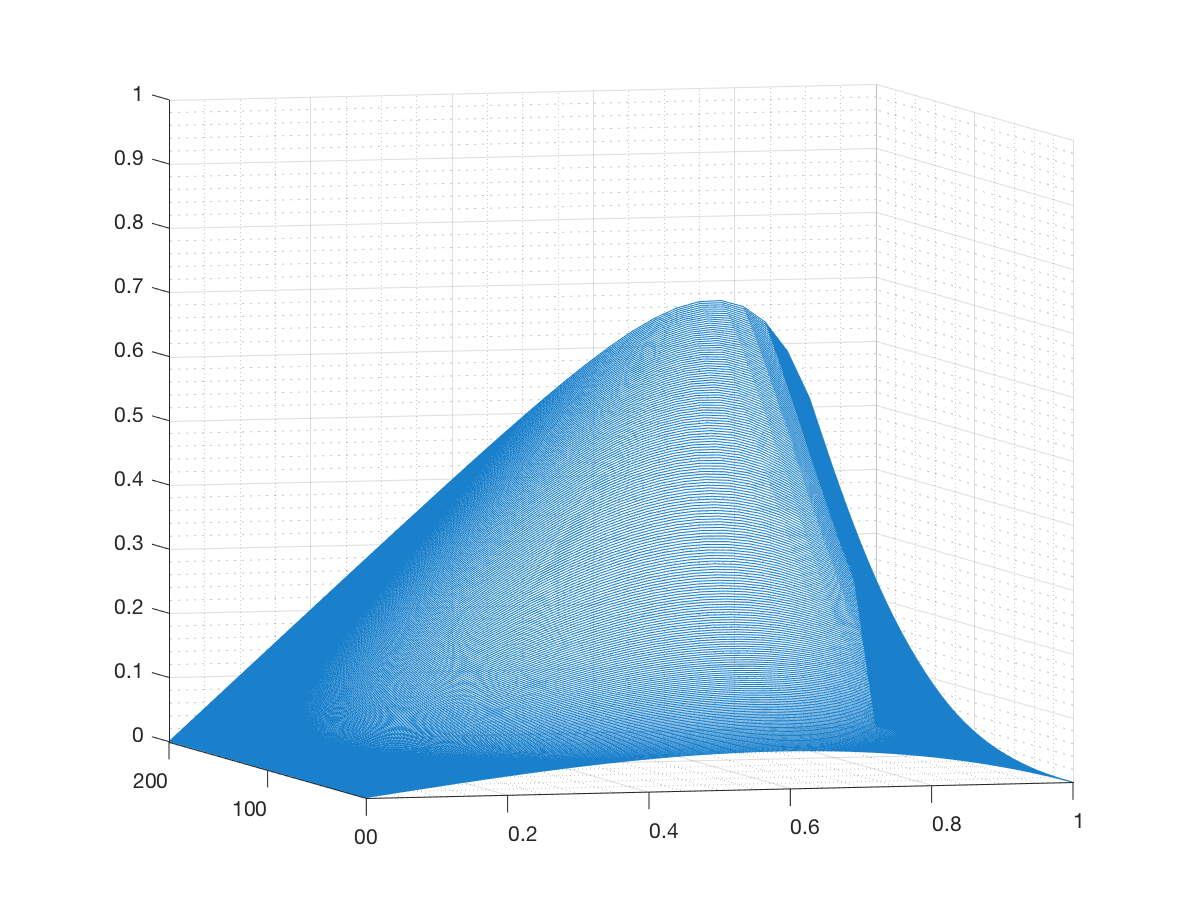
\includegraphics[width = 0.98\linewidth]{title_image}
	\end{center}
\end{figure}

\vspace{80pt}

\newpage

\tableofcontents

\newpage

\section{Model Problem}

The model second-order linear ordinary differential equation boundary-value problem consists of:
\begin{itemize}
	\item the second-order linear ordinary differential equation:
	\begin{equation}
	\pm u''(x)+k^2u(x)=k^2x \qquad x \in (0, 1)
	\end{equation}
	\item the boundary conditions:
	\begin{equation}
	u(0) = 0 \quad \textnormal{and} \quad u(1) = 0 
	\end{equation}
\end{itemize}
The model second-order linear ordinary differential equation is given with a plus-or-minus sign, as the results of the solution of each second-order linear ordinary differential equation are similar. The physical model of the positive case is that of the amplitude of standing waves for uniaxial forced vibration of a bar. The physical model for the negative case is that of (1) the temperature of a bar for uniaxial heat conduction, and (2) the deflection of a beam for uniaxial deformation with distributed elastic restraint.

\newpage

\section{Analytical Solution}

\subsection{Positive ODE}

The following equation is the positive second-order linear ordinary differential equation (ODE).
\begin{equation}
u''(x)+k^2u(x)=k^2x
\end{equation}

\subsubsection{Homogeneous Solution}

Let the homogeneous solution to the positive ODE be defined as $u_h(x)$. Then, $u_h(x)$ must satisfy the following homogeneous ODE.
\begin{equation}
u''_h(x) + k^2u_h(x) = 0
\end{equation}
The solution of the homogeneous ODE is assumed to be of the form: 
\begin{equation}
u_h(x) = e^{\lambda x}
\end{equation}
Taking the second-derivative of $u_h(x)$, substituting the second-derivative into the homogeneous ODE, and reducing the equation yields the \textbf{characteristic equation}.
\begin{equation}
u''_h(x) = \lambda^2 e^{\lambda x}
\end{equation}
\begin{equation}
\lambda^2 e^{\lambda x} + k^2e^{\lambda x} = 0
\end{equation}
\begin{equation}
\mathbf{\lambda^2 + k^2 = 0}
\end{equation}
Solving for $\lambda$ yields:
\begin{equation}
\lambda = \pm ik
\end{equation}
The homogenous solution $u_h(x)$ is then:
\begin{equation}
u_h(x) = \alpha e^{ikx} + \beta e^{-ikx}
\end{equation}
Making a transformation with the following relations, a more sophistocated solution can be developed:
\begin{equation}
\gamma = \frac{\alpha+\beta}{2} \quad \textnormal{and} \quad \delta = i\frac{\alpha-\beta}{2}
\end{equation}
\begin{equation}
u_h(x) = \gamma \frac{e^{ikx}+e^{-ikx}}{2} + \delta \frac{e^{ikx}-e^{-ikx}}{2i}
\end{equation}
\begin{equation}
\mathbf{u_h(x) = \gamma cos(kx) + \delta sin(kx)}
\end{equation}

\subsubsection{Particular Solution}

Let the particular solution to the positive ODE be defined as $u_p(x)$. Then, $u_p(x)$ must satisfy the ODE:
\begin{equation}
u''_p(x) + k^2u_p(x) = k^2x
\end{equation}
The second-derivative of $u_p(x)$, $u''_p(x)$, is assumed to be zero, and thus yields the particular solution $u_p(x)$:
\begin{equation}
k^2u_p(x) = k^2x
\end{equation}
\begin{equation}
\mathbf{u_p(x) = x}
\end{equation}

\subsubsection{Boundary Conditions}

Given that $u_h(x)$ is a solution to the homogeneous ODE and $u_p(x)$ is a solution to the ODE, then the combination of $u_h(x)$ and $u_p(x)$ is also a solution to the ODE.
\begin{equation}
u(x) = u_h(x) + u_p(x)
\end{equation}
\begin{equation}
u(x) = \gamma cos(kx) + \delta sin(kx) + x
\end{equation}
The boundary conditions for the model problem are:
\begin{equation}
u(0) = 0 \quad \textnormal{and} \quad u(1) = 0 
\end{equation}
Applying the first boundary condition, $u(0) = 0$, we get that $\gamma = 0$:
\begin{equation}
u(0) = 0 = \gamma cos(0) + \delta sin(0) + 0
\end{equation}
\begin{equation}
\gamma = 0
\end{equation}
Applying the second boundary condition, $u(1) = 0$, we get that $\delta = \frac{-1}{sin(k)}$:
\begin{equation}
u(1) = 0 = \delta sin(k) + 1
\end{equation}
\begin{equation}
\delta = \frac{-1}{sin(k)}
\end{equation}

\subsubsection{Analytical Solution}

Thus, it is shown that for the positive second-order linear ordinary differential equation with specified boundary conditions (reproduced below) that $u(x)$ is a solution to the differential equation on $x \in (0, 1)$.
\begin{equation}
u''(x)+k^2u(x)=k^2x \qquad x \in (0, 1)
\end{equation}
\begin{equation}
u(0) = 0 \quad \textnormal{and} \quad u(1) = 0 
\end{equation}
\begin{equation}
\mathbf{u(x) = x - \frac{sin(kx)}{sin(k)}}
\end{equation}

\subsection{Negative ODE}

The following equation is the negative second-order linear ordinary differential equation (ODE).
\begin{equation}
-u''(x)+k^2u(x)=k^2x
\end{equation}

\subsubsection{Homogeneous Solution}

Let the homogeneous solution to the negative ODE be defined as $u_h(x)$. Then, $u_h(x)$ must satisfy the following homogeneous ODE.
\begin{equation}
-u''_h(x) + k^2u_h(x) = 0
\end{equation}
The solution of the homogeneous ODE is assumed to be of the form: 
\begin{equation}
u_h(x) = e^{\lambda x}
\end{equation}
Taking the second-derivative of $u_h(x)$, substituting the second-derivative into the homogeneous ODE, and reducing the equation yields the \textbf{characteristic equation}.
\begin{equation}
u''_h = \lambda^2 e^{\lambda x}
\end{equation}
\begin{equation}
-\lambda^2 e^{\lambda x} + k^2e^{\lambda x} = 0
\end{equation}
\begin{equation}
\mathbf{-\lambda^2 + k^2 = 0}
\end{equation}
Solving for $\lambda$ yields:
\begin{equation}
\lambda = \pm k
\end{equation}
The homogenous solution $u_h(x)$ is then:
\begin{equation}
u_h(x) = \alpha e^{kx} + \beta e^{-kx}
\end{equation}
By making a transformation with the following relations, a more sophistocated solution can be developed:
\begin{equation}
\gamma = \frac{\alpha+\beta}{2} \quad \textnormal{and} \quad \delta = \frac{\alpha-\beta}{2}
\end{equation}
\begin{equation}
u_h(x) = \gamma \frac{e^{kx}+e^{-kx}}{2} + \delta \frac{e^{kx}-e^{-kx}}{2}
\end{equation}
\begin{equation}
\mathbf{u_h(x) = \gamma cosh(kx) + \delta sinh(kx)}
\end{equation}

\subsubsection{Particular Solution}

Let the particular solution to the negative ODE be defined as $u_p(x)$. Then, $u_p(x)$ must satisfy the ODE:
\begin{equation}
-u''_p(x) + k^2u_p(x) = k^2x
\end{equation}
The second-derivative of $u_p(x)$, $u''_p(x)$, is assumed to be zero, and thus yields the particular solution $u_p(x)$:
\begin{equation}
k^2u_p(x) = k^2x
\end{equation}
\begin{equation}
\mathbf{u_p(x) = x}
\end{equation}

\subsubsection{Boundary Conditions}

Given that $u_h(x)$ is a solution to the homogeneous ODE and $u_p(x)$ is a solution to the ODE, then the combination of $u_h(x)$ and $u_p(x)$ is also a solution to the ODE.
\begin{equation}
u(x) = u_h(x) + u_p(x)
\end{equation}
\begin{equation}
u(x) = \gamma cosh(kx) + \delta sinh(kx) + x
\end{equation}
The boundary conditions for the model problem are:
\begin{equation}
u(0) = 0 \quad \textnormal{and} \quad u(1) = 0 
\end{equation}
Applying the first boundary condition, $u(0) = 0$, we get that $\gamma = 0$:
\begin{equation}
u(0) = 0 = \gamma cosh(0) + \delta sinh(0) + 0
\end{equation}
\begin{equation}
\gamma = 0
\end{equation}
Applying the second boundary condition, $u(1) = 0$, we get that $\delta = \frac{-1}{sinh(k)}$:
\begin{equation}
u(1) = 0 = \delta sinh(k) + 1
\end{equation}
\begin{equation}
\delta = \frac{-1}{sinh(k)}
\end{equation}

\subsubsection{Analytical Solution}

Thus, it is shown that for the negative second-order linear ordinary differential equation with specified boundary conditions (reproduced below) that $u(x)$ is a solution to the differential equation on $x \in (0, 1)$.
\begin{equation}
-u''(x)+k^2u(x)=k^2x \qquad x \in (0, 1)
\end{equation}
\begin{equation}
u(0) = 0 \quad \textnormal{and} \quad u(1) = 0 
\end{equation}
\begin{equation}
\mathbf{u(x) = x - \frac{sinh(kx)}{sinh(k)}}
\end{equation}

\newpage

\section{Numerical Methods}

\subsection{Derivations}

\subsubsection{Second-Order Second-Derivative Finite Difference Method}

Developing the Taylor series for $u(x)$ in the vicinity of $x = i$:
\begin{equation}
u_{i-1} = u_i - \Delta x u'_i + \frac{\Delta x^2}{2} u''_i - \frac{\Delta x^3}{6} u^{(3)}_i + \frac{\Delta x^4}{24} u^{(4)}_i + \mathcal{O}(\Delta x^5)
\end{equation}
\begin{equation}
u_{i+1} = u_i + \Delta x u'_i + \frac{\Delta x^2}{2} u''_i + \frac{\Delta x^3}{6} u^{(3)}_i + \frac{\Delta x^4}{24} u^{(4)}_i + \mathcal{O}(\Delta x^5)
\end{equation}
Adding the Taylor series for $u_{i-1}$ and $u_{i+1}$ and canceling terms:
\begin{equation}
u_{i+1} + u_{i-1} = 2u_i + \Delta x^2 u''_i + \mathcal{O}(\Delta x^4)
\end{equation}
Rearranging terms to solve for $u''_i$:
\begin{equation}
u''_i = \frac{u_{i+1} - 2u_i + u_{i-1}}{\Delta x^2} + \mathcal{O}(\Delta x^2) 
\end{equation}

From this specific second-derivative formulation using the finite difference method, the approximation can be observed to be second-order ($\mathcal{O}(\Delta x^2)$).

\subsubsection{Fourth-Order Second-Derivative Finite Difference Method}

Developing the Taylor series for $u(x)$ in the vicinity of $x = i$:
\begin{equation}
u_{i-1} = u_i - \Delta x u'_i + \frac{\Delta x^2}{2} u''_i - \frac{\Delta x^3}{6} u^{(3)}_i + \frac{\Delta x^4}{24} u^{(4)}_i + \mathcal{O}(\Delta x^5)
\end{equation}
\begin{equation}
u_{i+1} = u_i + \Delta x u'_i + \frac{\Delta x^2}{2} u''_i + \frac{\Delta x^3}{6} u^{(3)}_i + \frac{\Delta x^4}{24} u^{(4)}_i + \mathcal{O}(\Delta x^5)
\end{equation}
Adding the Taylor series for $u_{i-1}$ and $u_{i+1}$ and canceling terms:
\begin{equation}
u_{i+1} + u_{i-1} = 2u_i + \Delta x^2 u''_i + \frac{\Delta x^4}{12} u^{(4)}_i + \mathcal{O}(\Delta x^6)
\end{equation}
Rearranging for $u''_i$, we get:
\begin{equation}
u''_i = \frac{u_{i+1} -2u_i + u_{i-1}}{\Delta x^2} - \frac{\Delta x^2}{12} u^{(4)}_i + \mathcal{O}(\Delta x^4)
\end{equation}
Returning to the differential equation and then taking two additional derivatives, we can arrive at an expression for $u^{(4)}_i$, with the sign given with opposite correspondence to the sign of the differential equation:
\begin{equation}
\pm u''(x)+k^2u(x)=k^2x \qquad x \in (0, 1)
\end{equation}
\begin{equation}
\pm u^{(4)}(x)+k^2u''(x)=0
\end{equation}
\begin{equation}
u^{(4)}(x) = \mp k^2u''(x)
\end{equation}
Substituting in the fourth-derivative expression:
\begin{equation}
u''_i = \frac{u_{i+1} -2u_i + u_{i-1}}{\Delta x^2} \pm \frac{\Delta x^2}{12} k^2u''_i + \mathcal{O}(\Delta x^4)
\end{equation}
Now, exchanging the $u''_i$ term with the earlier derivation and simplifying:
\begin{equation}
u''_i = \frac{u_{i+1} -2u_i + u_{i-1}}{\Delta x^2} \pm \frac{\Delta x^2}{12} k^2 \left[\frac{u_{i+1} -2u_i + u_{i-1}}{\Delta x^2} + \mathcal{O}(\Delta x^2) \right] + \mathcal{O}(\Delta x^4)
\end{equation}
\begin{equation}
u''_i = \frac{1}{\Delta x^2} (u_{i+1} -2u_i + u_{i-1}) \pm \frac{k^2}{12} (u_{i+1} -2u_i + u_{i-1}) + \mathcal{O}(\Delta x^4)
\end{equation}
\begin{equation}
u''_i = \left(\frac{1}{\Delta x^2} \pm \frac{k^2}{12}\right) (u_{i+1} -2u_i + u_{i-1}) + \mathcal{O}(\Delta x^4)
\end{equation}
From this specific second-derivative formulation using the finite difference method, the approximation can be observed to be fourth-order ($\mathcal{O}(\Delta x^4)$).

\newpage

\subsection{Results}

\subsubsection{Positive ODE}

\begin{figure}[H]
	\begin{center}
		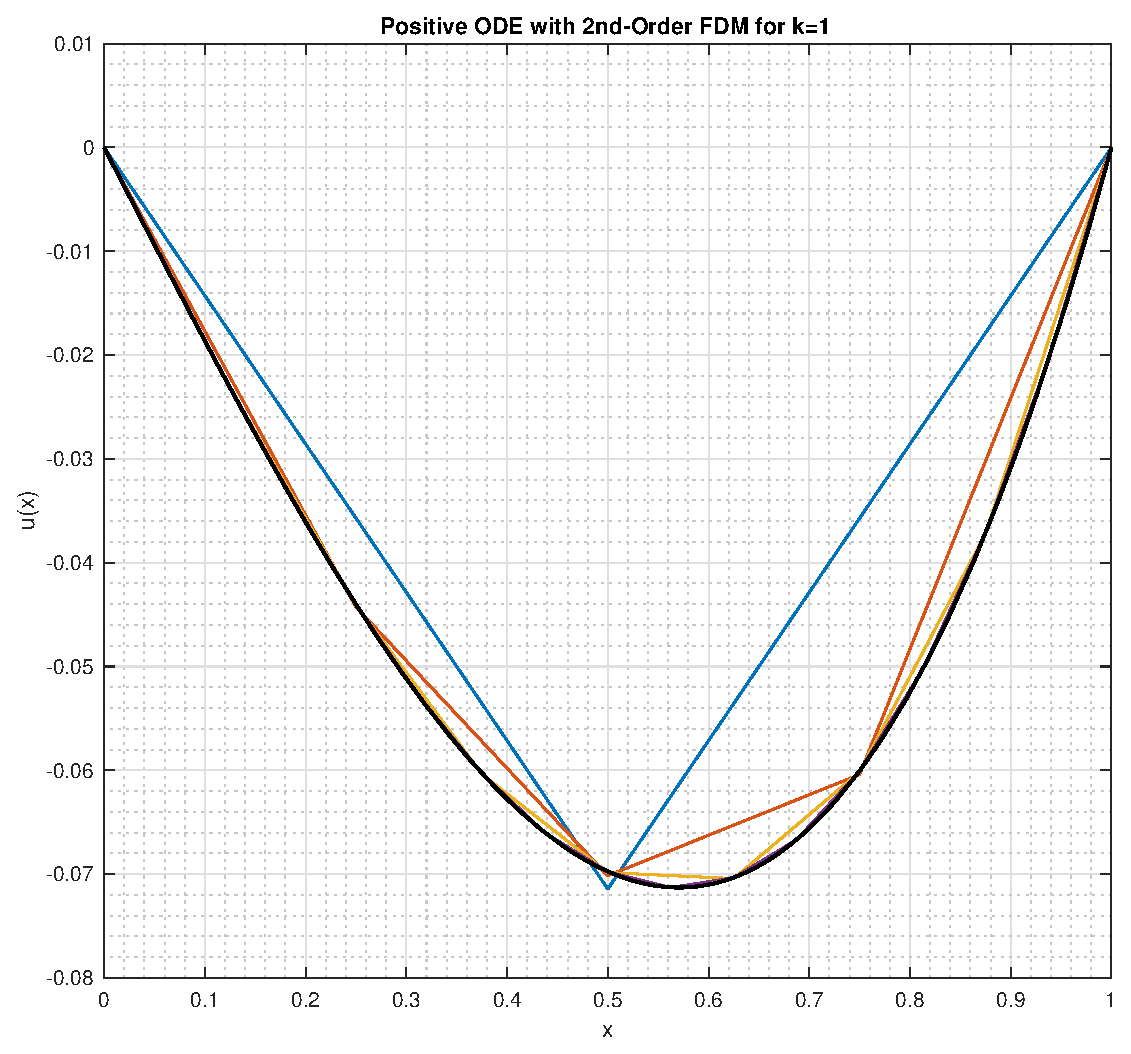
\includegraphics[width = 0.49\linewidth]{positive_ode_order_2_k_1}
		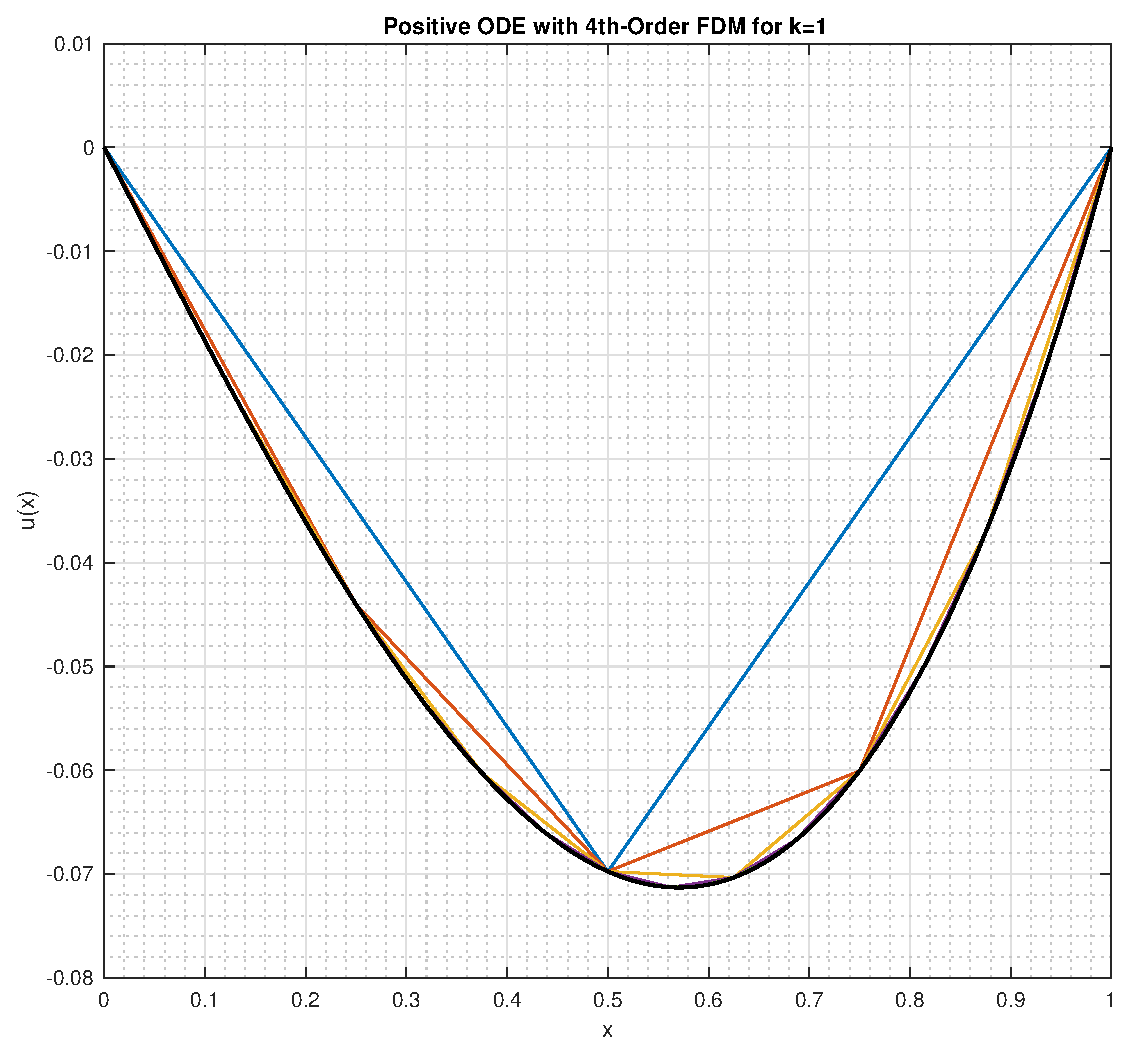
\includegraphics[width = 0.49\linewidth]{positive_ode_order_4_k_1}
		\caption{Positive ODE -- 2nd-Order and 4th-Order FDM for $k = 1$}
	\end{center}
\end{figure}

\begin{figure}[H]
	\begin{center}
		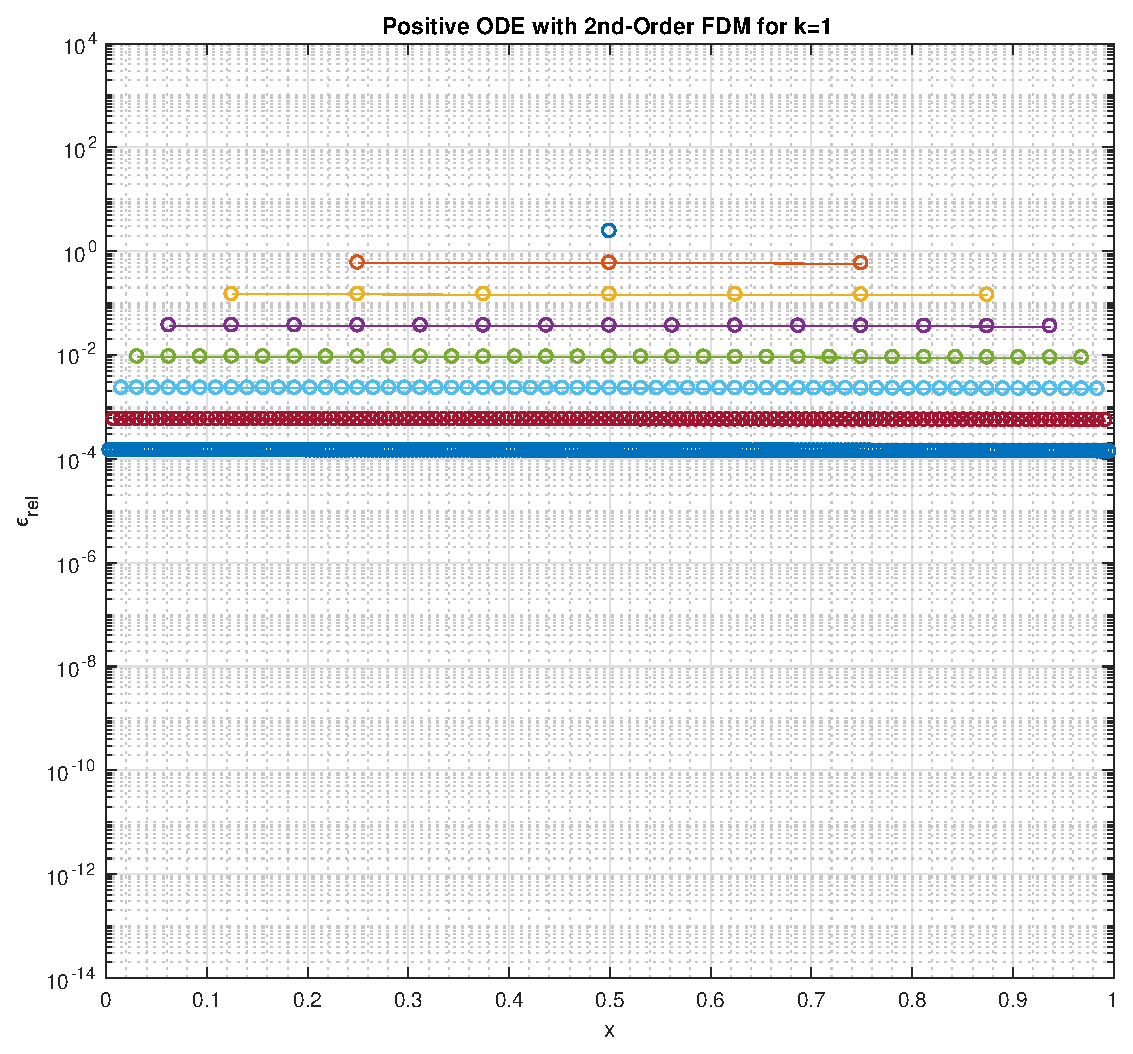
\includegraphics[width = 0.49\linewidth]{error_positive_ode_order_2_k_1}
		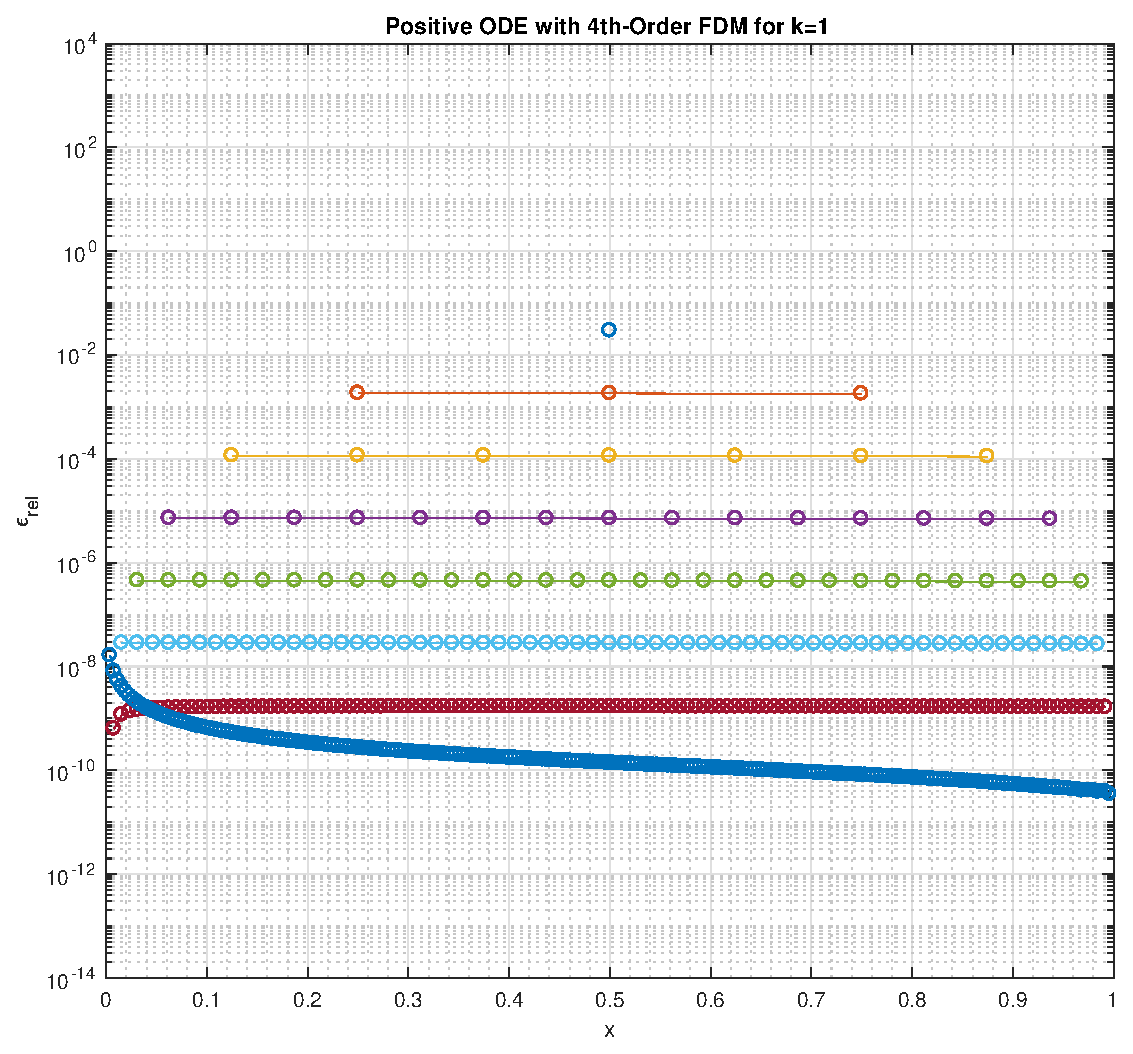
\includegraphics[width = 0.49\linewidth]{error_positive_ode_order_4_k_1}
		\caption{Pointwise Error -- Positive ODE -- 2nd-Order and 4th-Order FDM for $k = 1$}
	\end{center}
\end{figure}

\begin{center}
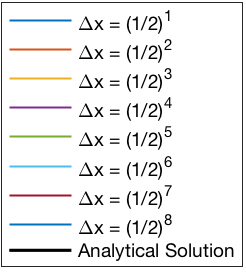
\includegraphics[height = 0.13\linewidth]{legend}
\end{center}

\newpage

\begin{figure}[H]
	\begin{center}
		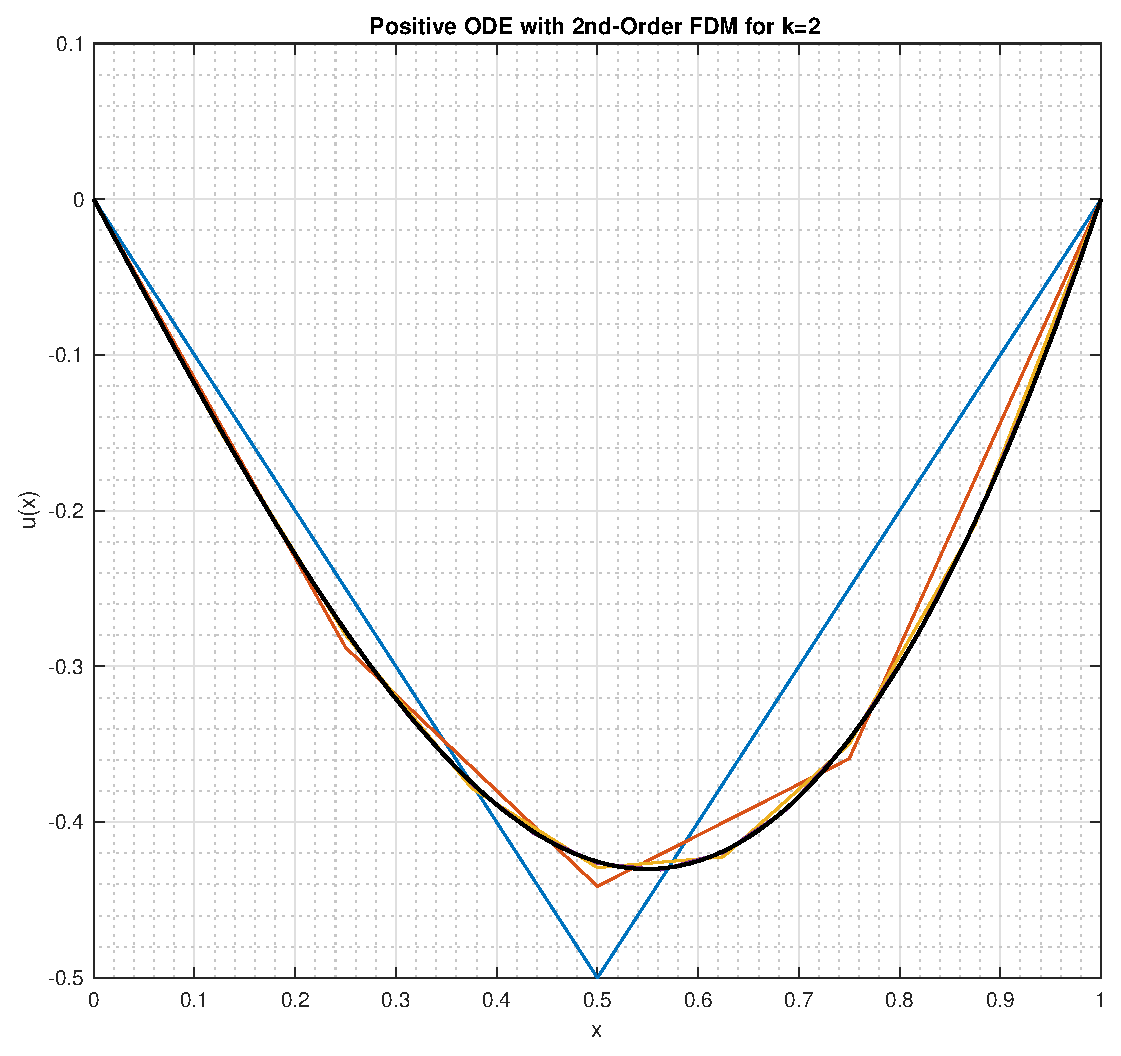
\includegraphics[width = 0.49\linewidth]{positive_ode_order_2_k_2}
		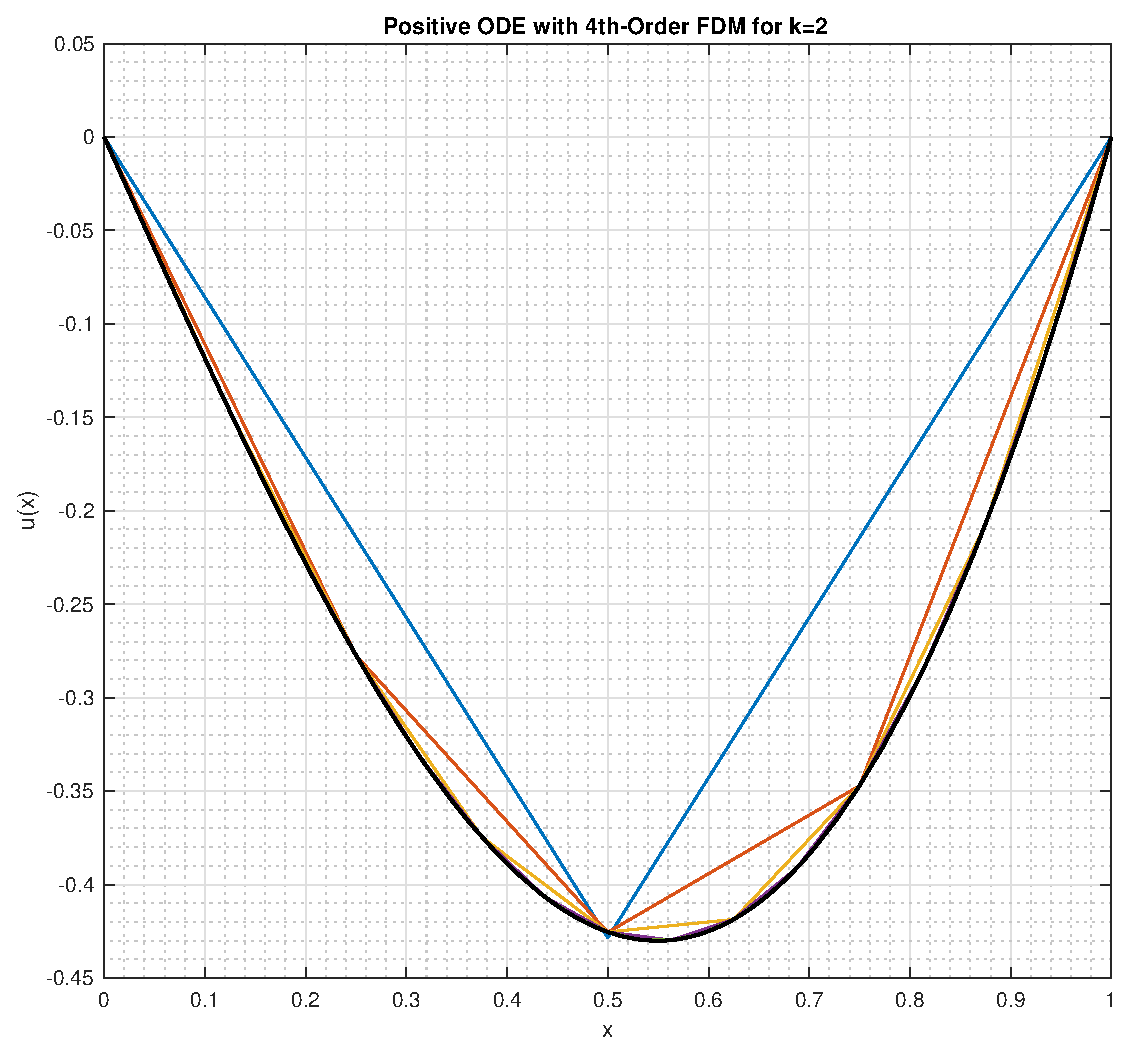
\includegraphics[width = 0.49\linewidth]{positive_ode_order_4_k_2}
		\caption{Positive ODE -- 2nd-Order and 4th-Order FDM for $k = 2$}
	\end{center}
\end{figure}

\begin{figure}[H]
	\begin{center}
		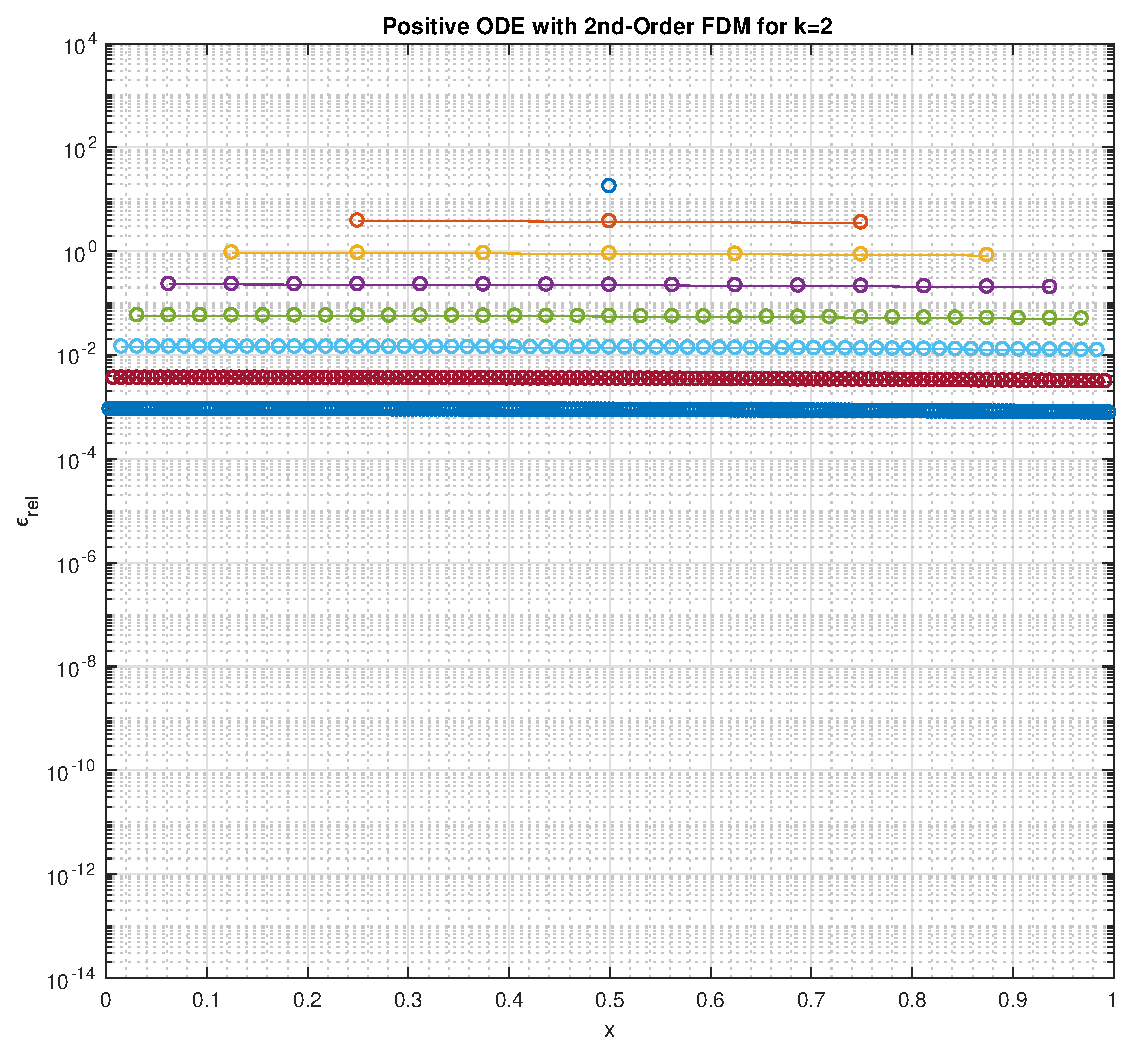
\includegraphics[width = 0.49\linewidth]{error_positive_ode_order_2_k_2}
		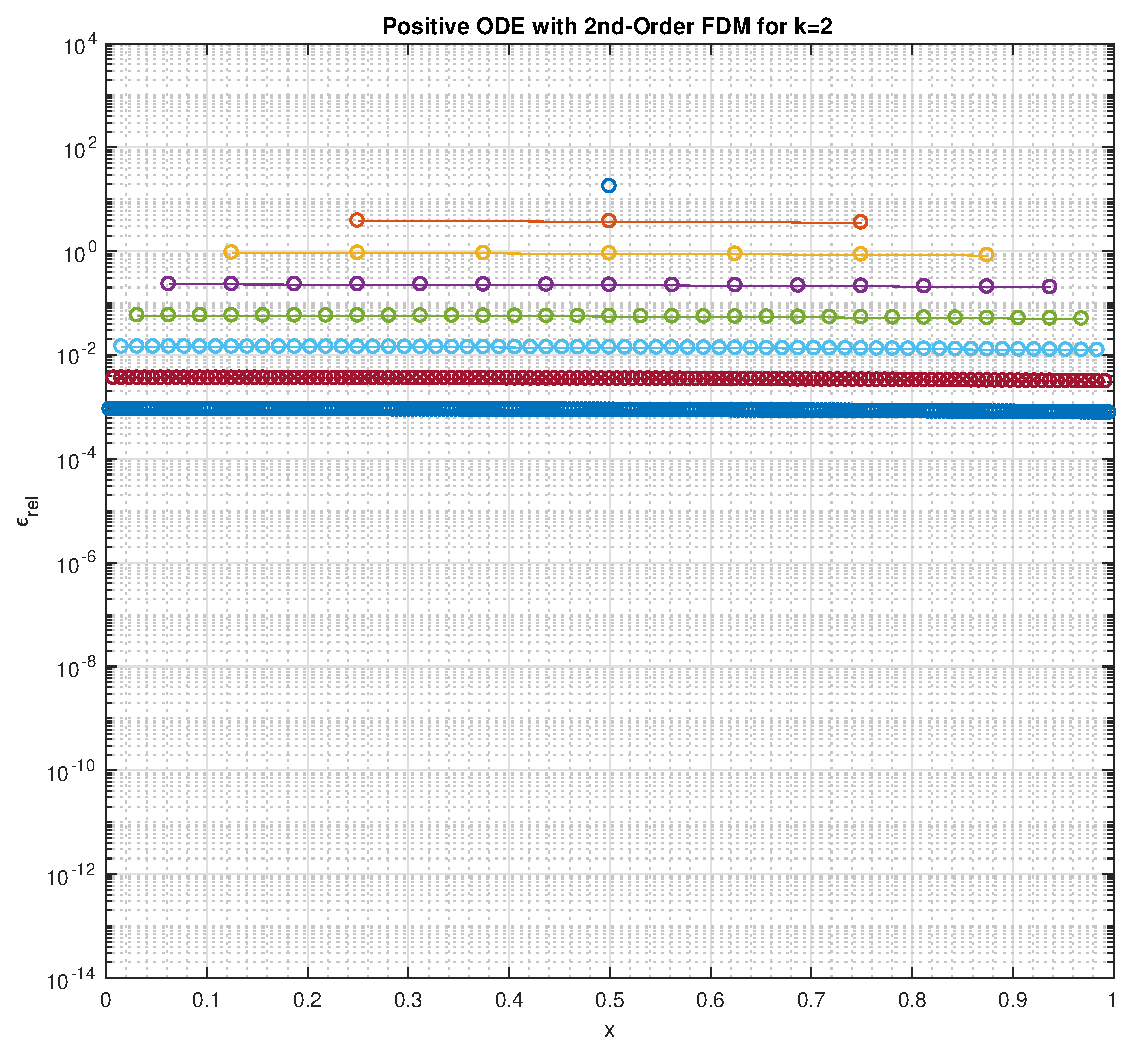
\includegraphics[width = 0.49\linewidth]{error_positive_ode_order_2_k_2}
		\caption{Pointwise Error -- Positive ODE -- 2nd-Order and 4th-Order FDM for $k = 2$}
	\end{center}
\end{figure}

\begin{center}
	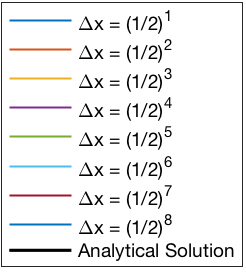
\includegraphics[height = 0.25\linewidth]{legend}
\end{center}

\newpage

\begin{figure}[H]
	\begin{center}
		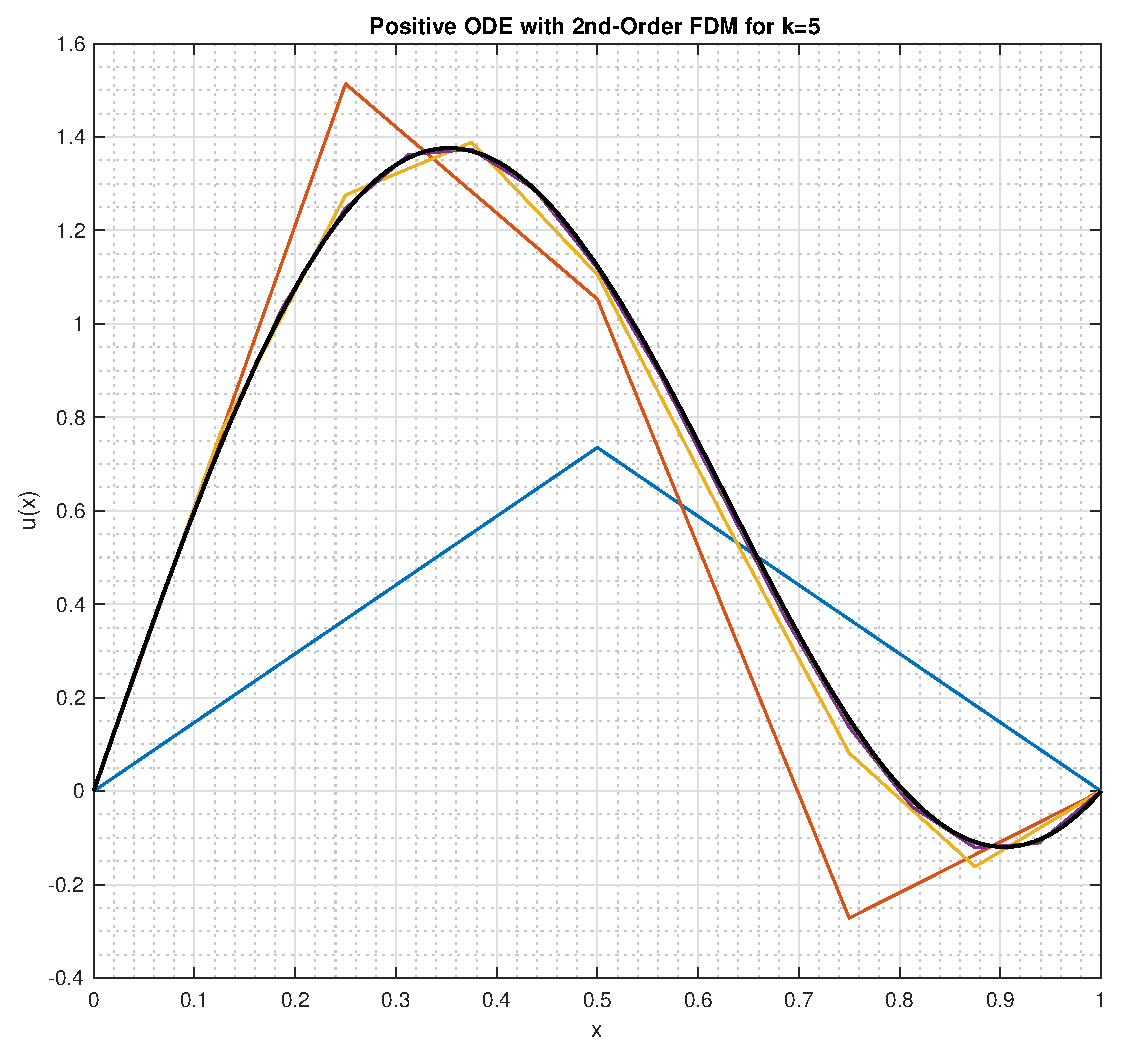
\includegraphics[width = 0.49\linewidth]{positive_ode_order_2_k_5}
		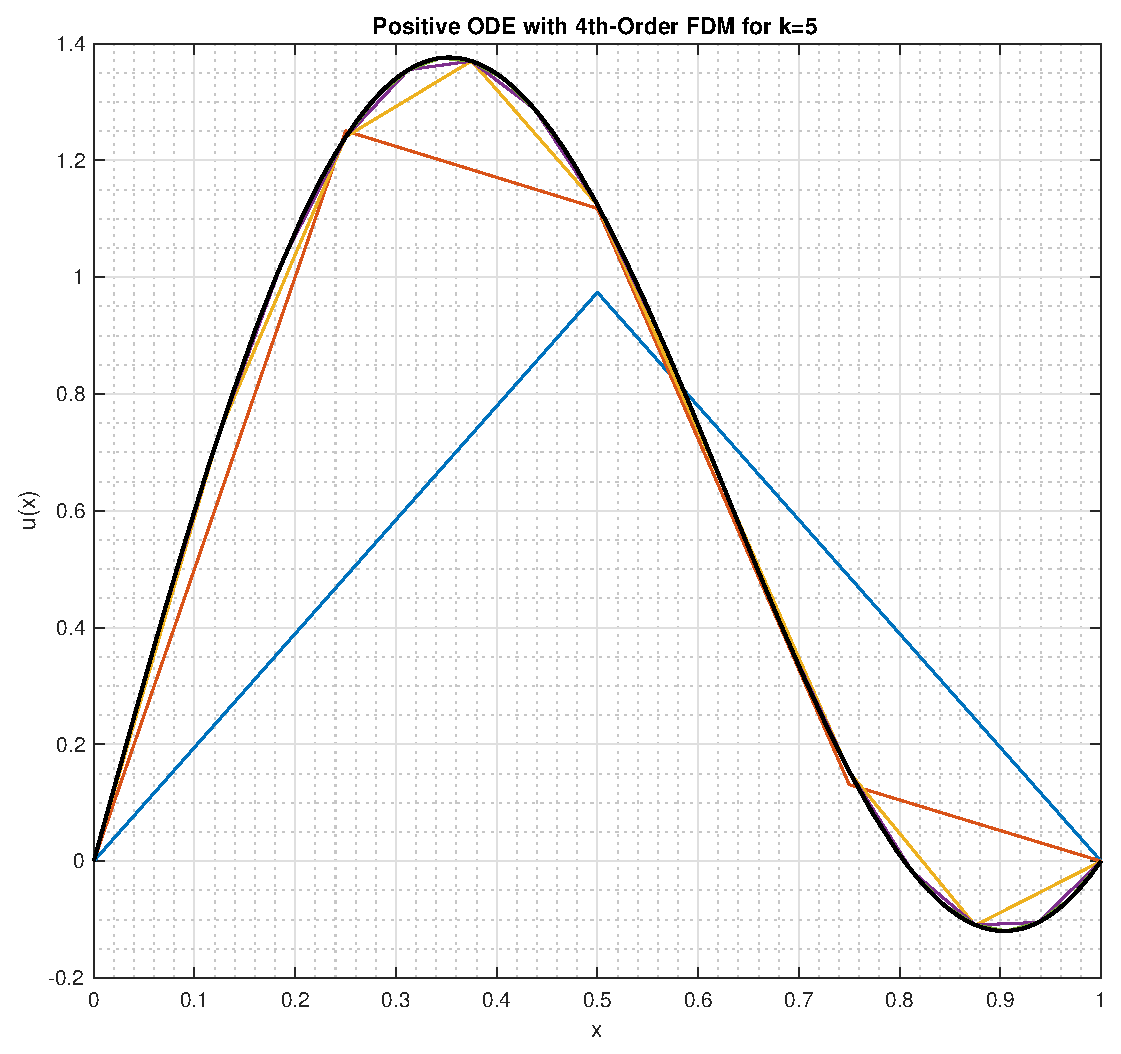
\includegraphics[width = 0.49\linewidth]{positive_ode_order_4_k_5}
		\caption{Positive ODE -- 2nd-Order and 4th-Order FDM for $k = 5$}
	\end{center}
\end{figure}

\begin{figure}[H]
	\begin{center}
		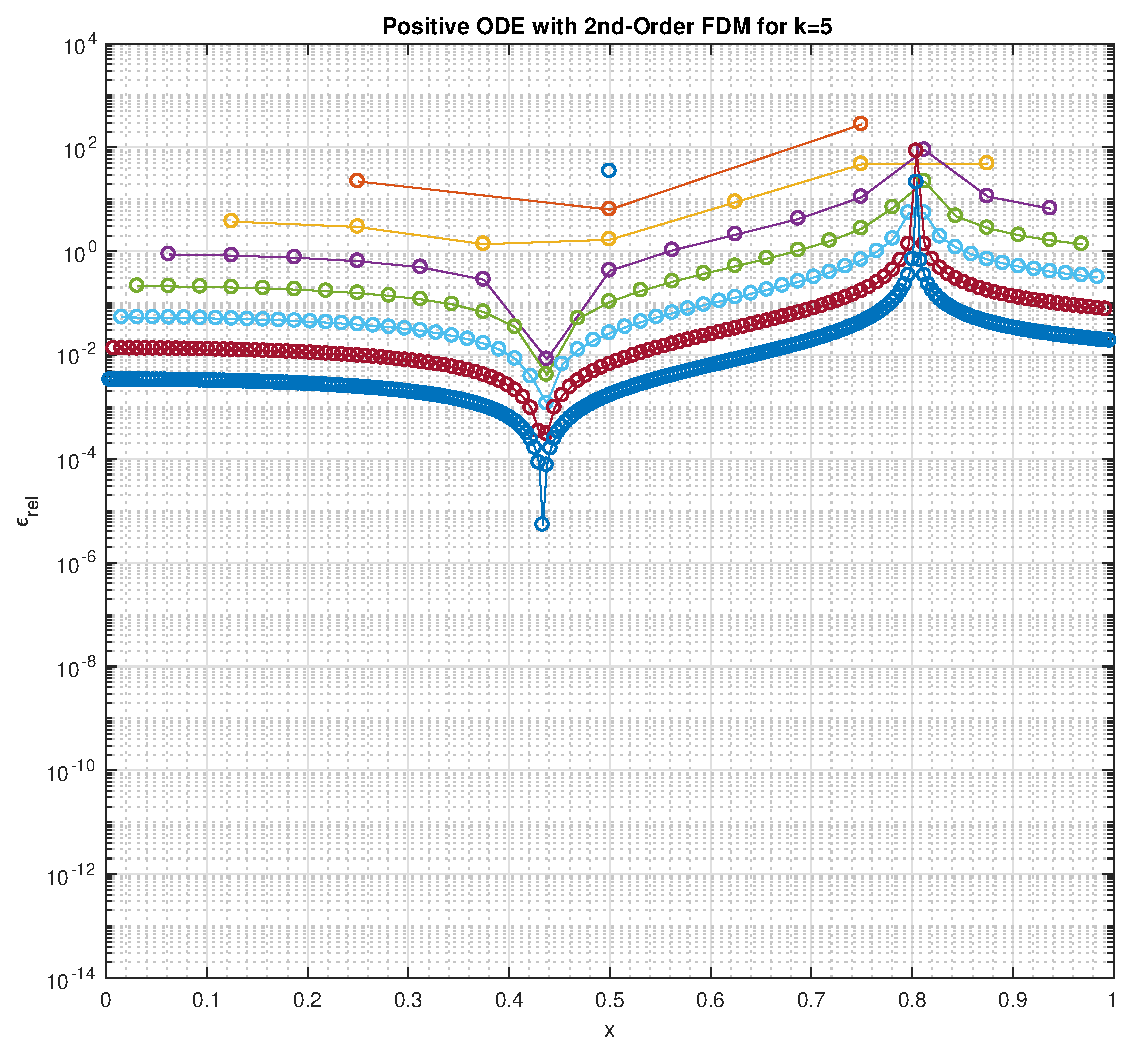
\includegraphics[width = 0.49\linewidth]{error_positive_ode_order_2_k_5}
		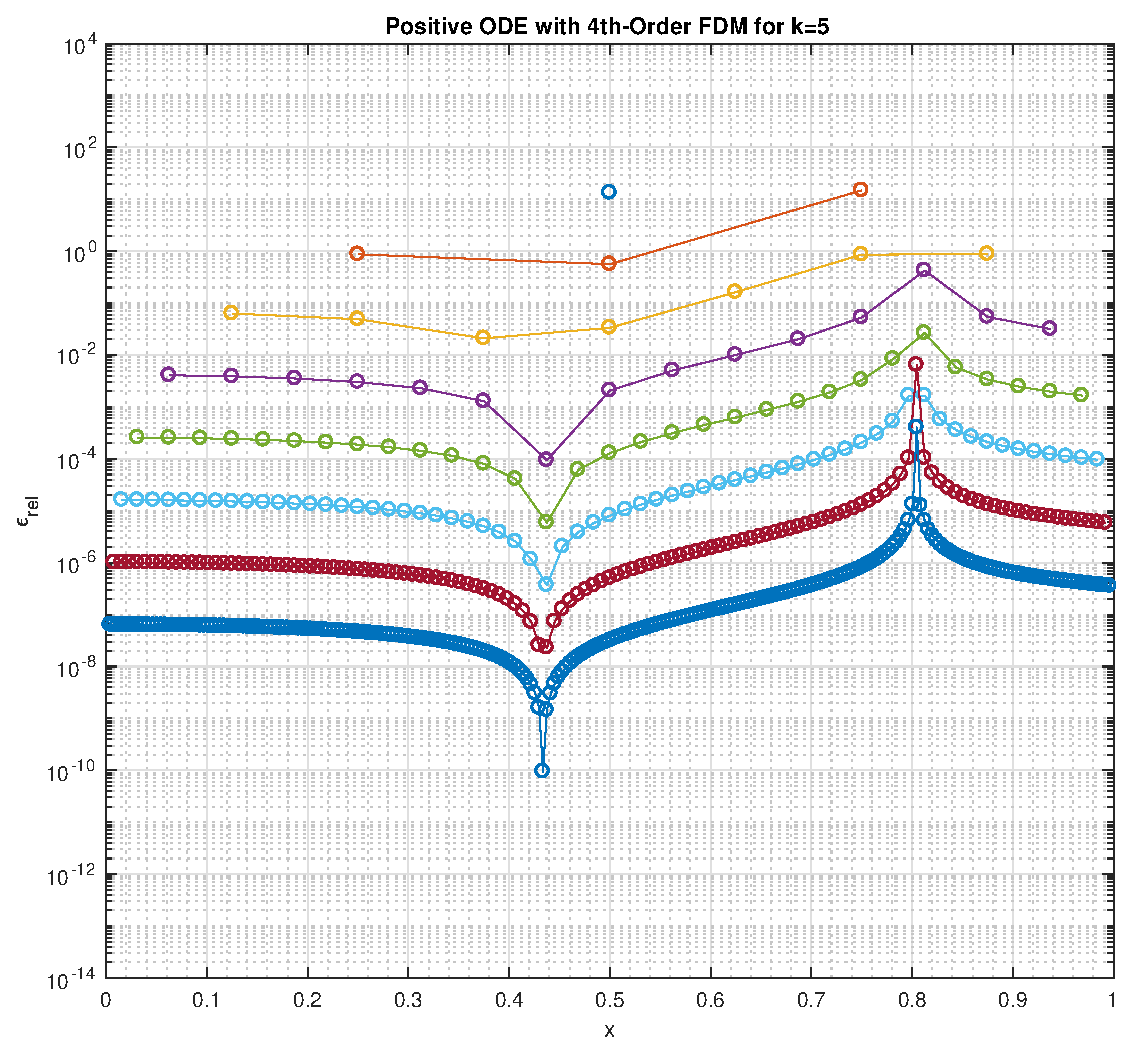
\includegraphics[width = 0.49\linewidth]{error_positive_ode_order_4_k_5}
		\caption{Pointwise Error -- Positive ODE -- 2nd-Order and 4th-Order FDM for $k = 5$}
	\end{center}
\end{figure}

\begin{center}
	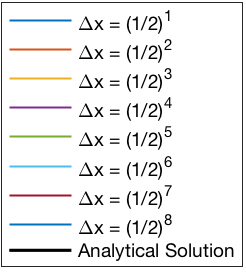
\includegraphics[height = 0.25\linewidth]{legend}
\end{center}

\newpage

\begin{figure}[H]
\begin{center}
	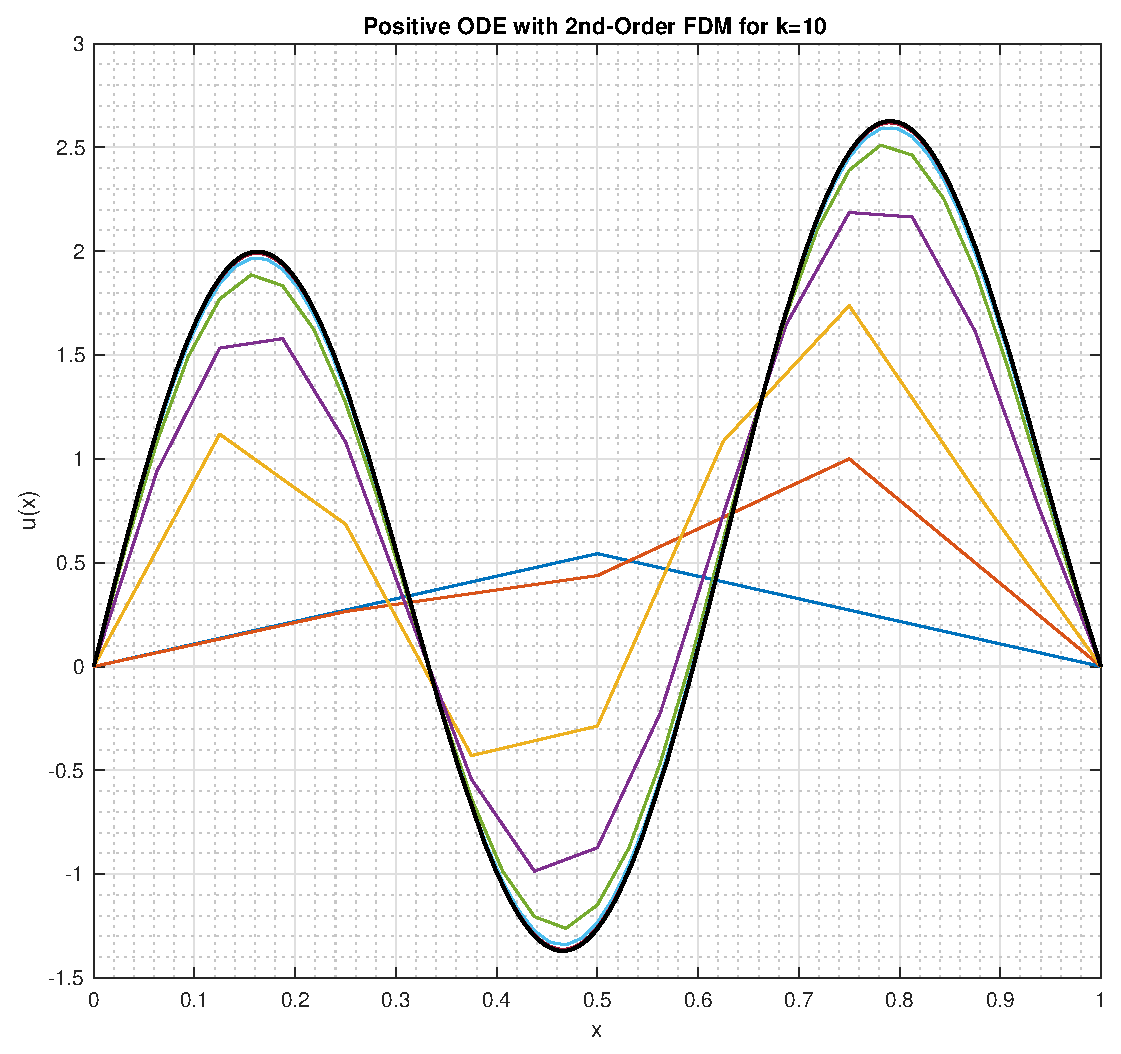
\includegraphics[width = 0.49\linewidth]{positive_ode_order_2_k_10}
	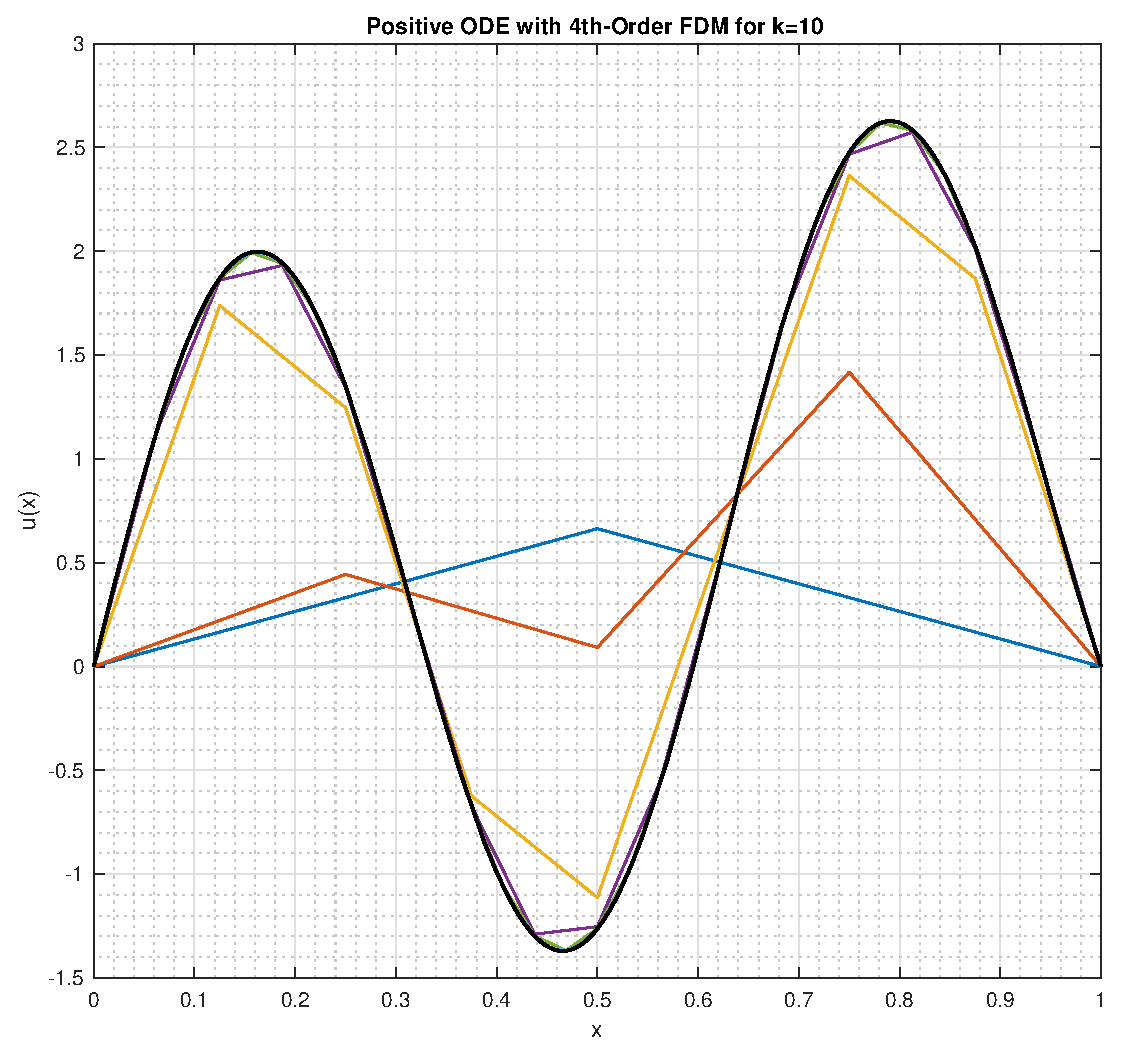
\includegraphics[width = 0.49\linewidth]{positive_ode_order_4_k_10}
	\caption{Positive ODE -- 2nd-Order and 4th-Order FDM for $k = 10$}
\end{center}
\end{figure}

\begin{figure}[H]
\begin{center}
	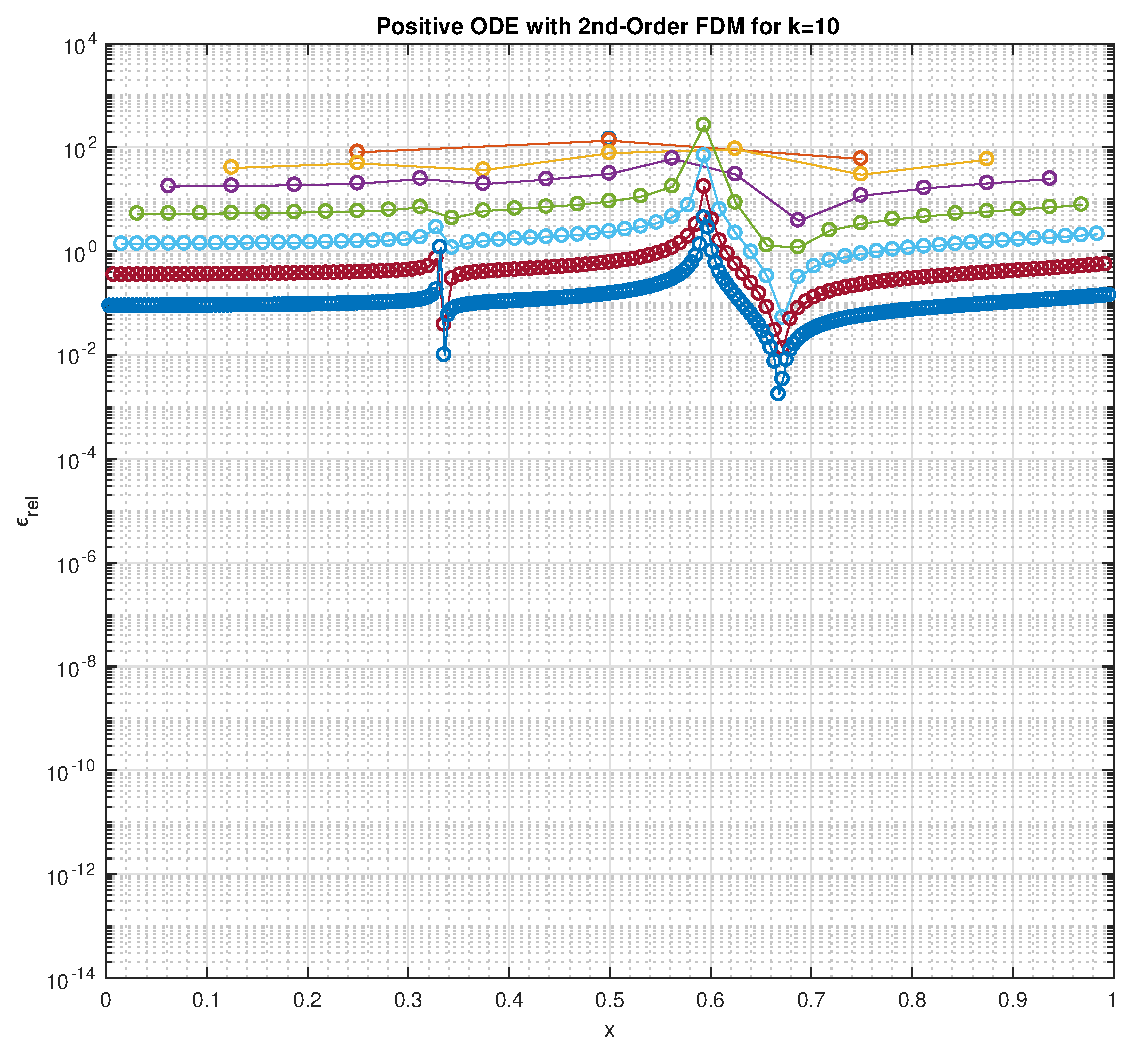
\includegraphics[width = 0.49\linewidth]{error_positive_ode_order_2_k_10}
	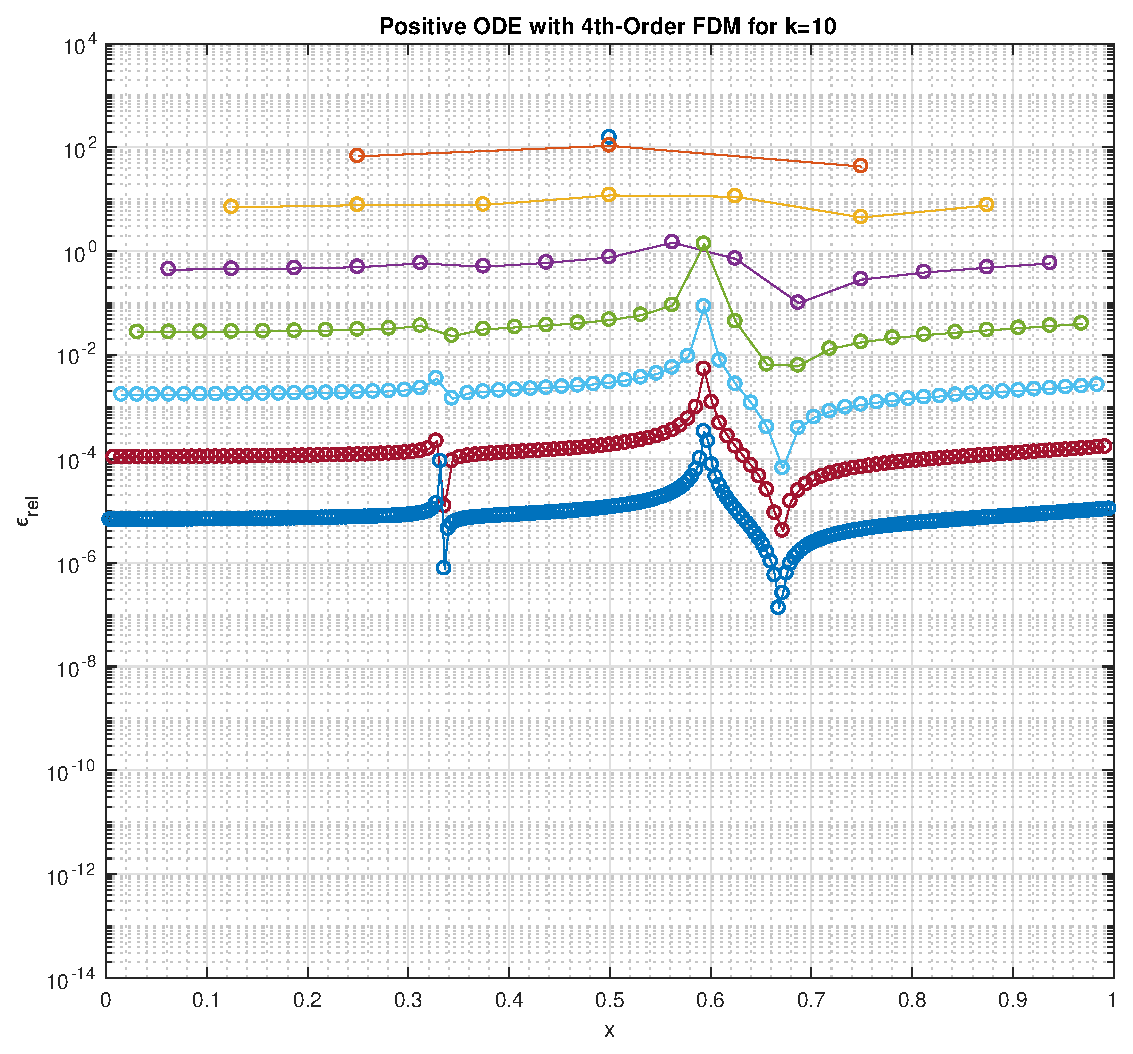
\includegraphics[width = 0.49\linewidth]{error_positive_ode_order_4_k_10}
	\caption{Pointwise Error -- Positive ODE -- 2nd-Order and 4th-Order FDM for $k = 10$}
\end{center}
\end{figure}

\begin{center}
	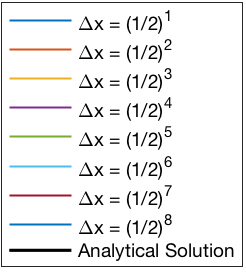
\includegraphics[height = 0.25\linewidth]{legend}
\end{center}

\newpage

\begin{figure}[H]
\begin{center}
	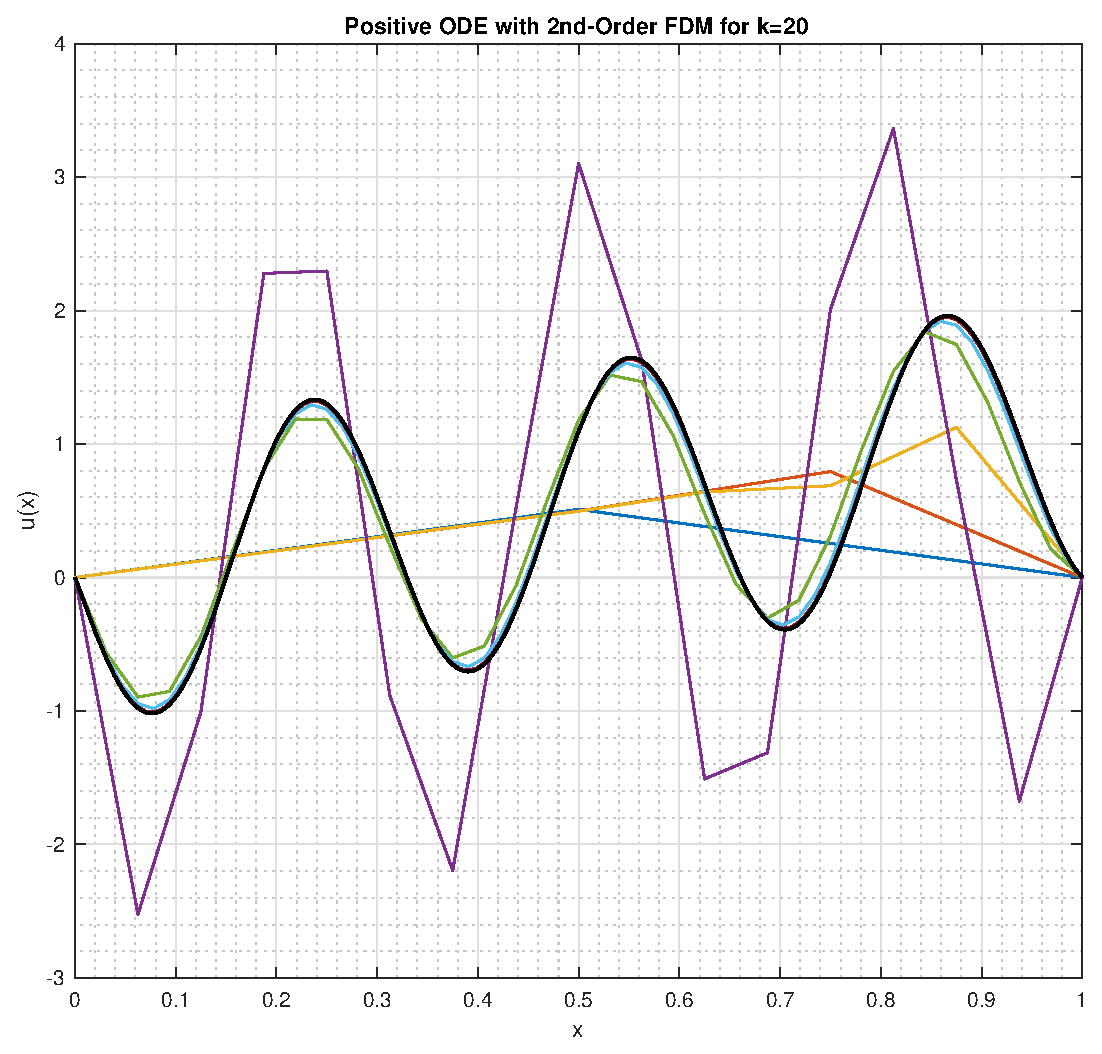
\includegraphics[width = 0.49\linewidth]{positive_ode_order_2_k_20}
	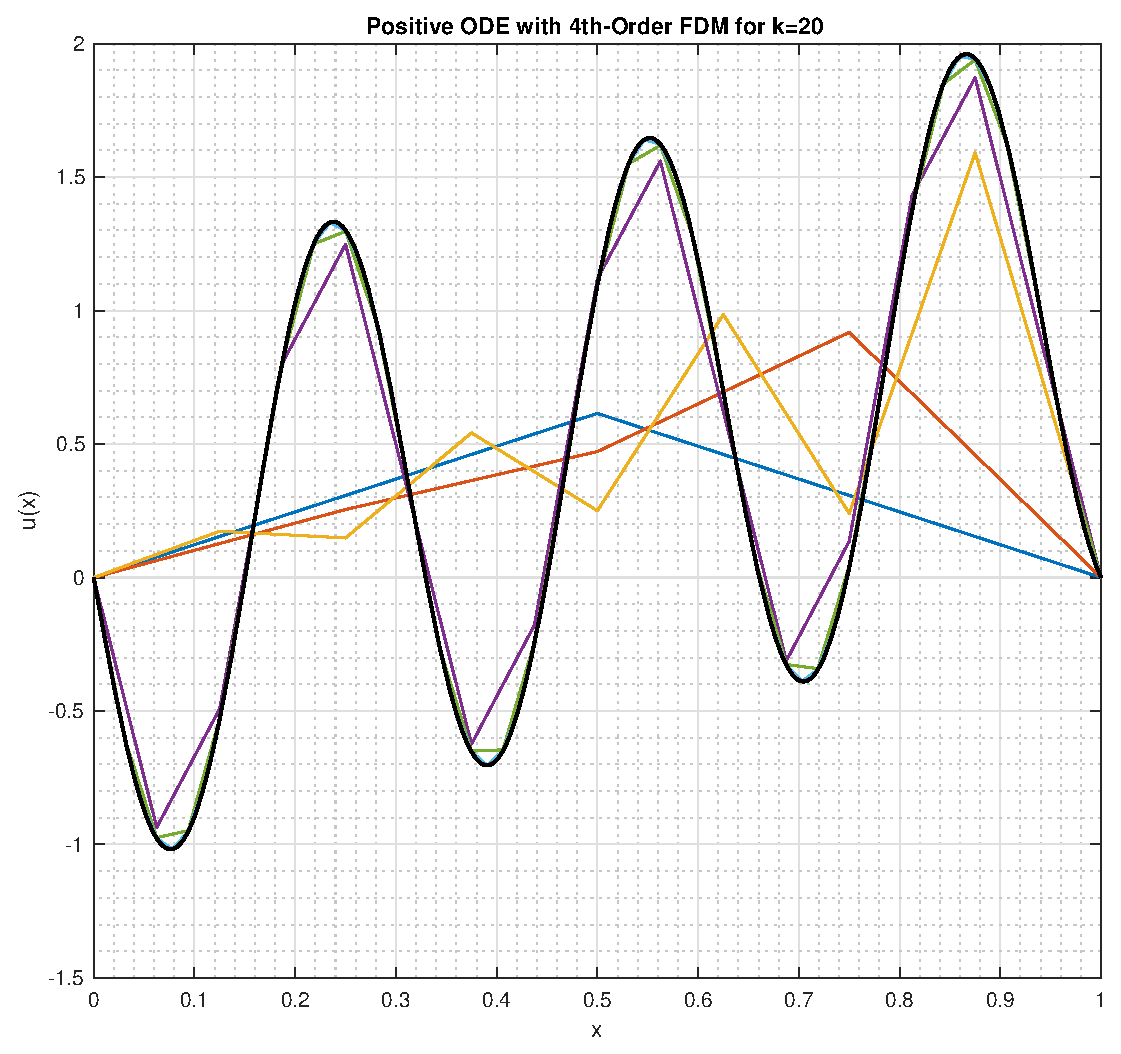
\includegraphics[width = 0.49\linewidth]{positive_ode_order_4_k_20}
	\caption{Positive ODE -- 2nd-Order and 4th-Order FDM for $k = 20$}
\end{center}
\end{figure}

\begin{figure}[H]
\begin{center}
	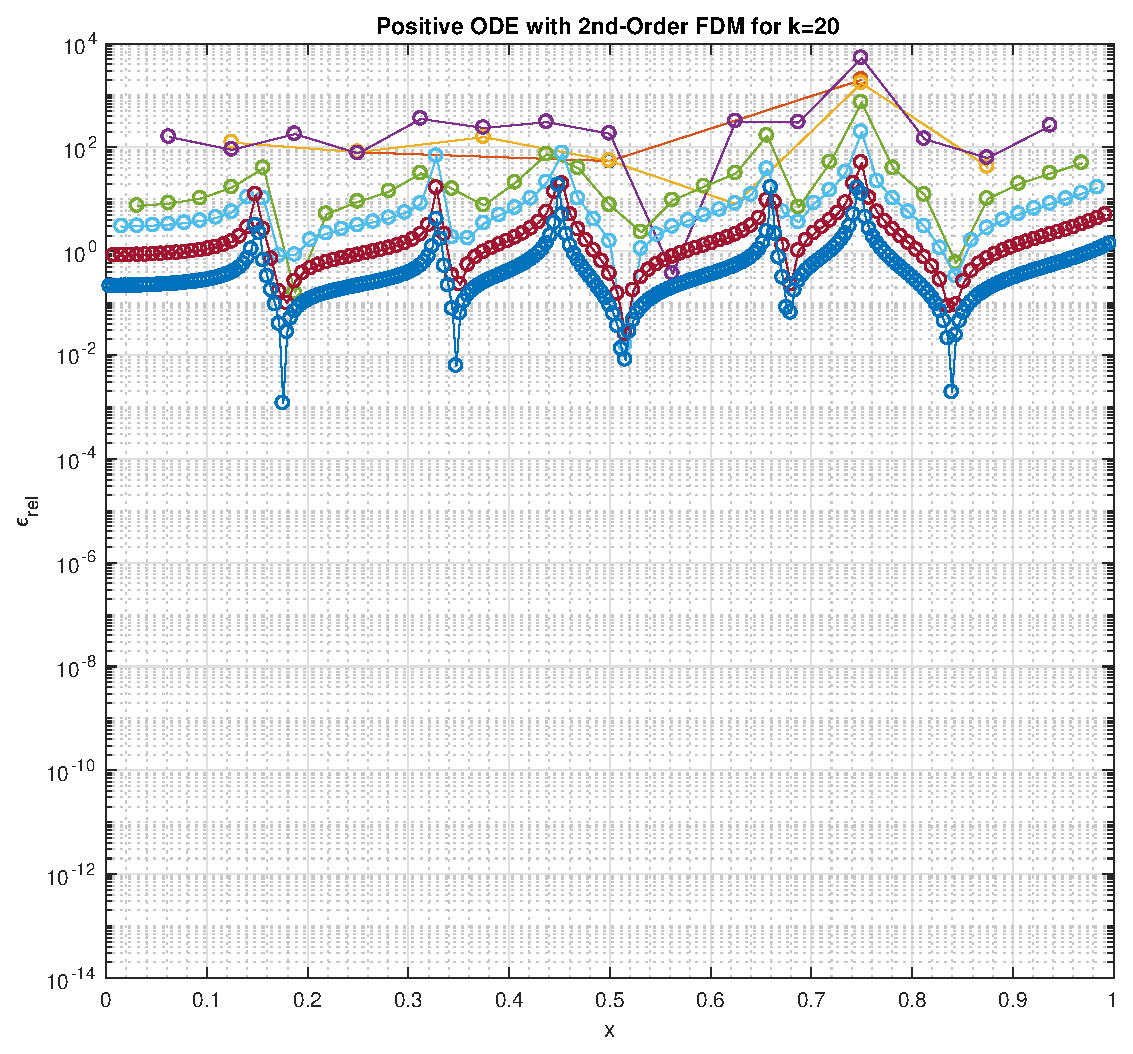
\includegraphics[width = 0.49\linewidth]{error_positive_ode_order_2_k_20}
	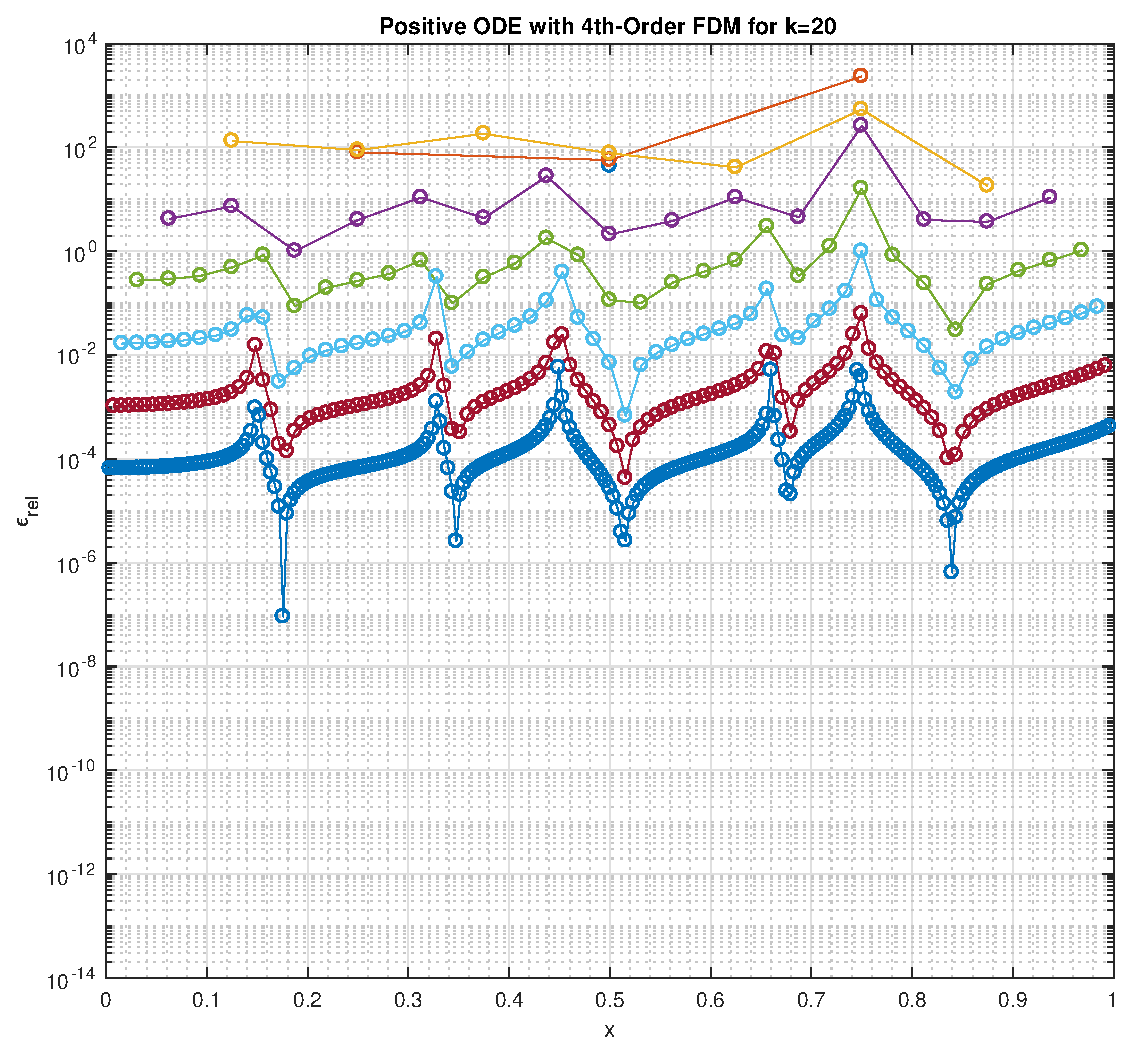
\includegraphics[width = 0.49\linewidth]{error_positive_ode_order_4_k_20}
	\caption{Pointwise Error -- Positive ODE -- 2nd-Order and 4th-Order FDM for $k = 20$}
\end{center}
\end{figure}

\begin{center}
	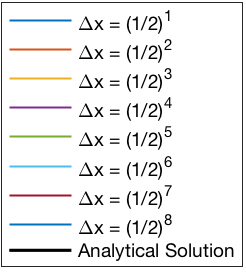
\includegraphics[height = 0.25\linewidth]{legend}
\end{center}

\newpage

\subsubsection{Negative ODE}

\begin{figure}[H]
	\begin{center}
		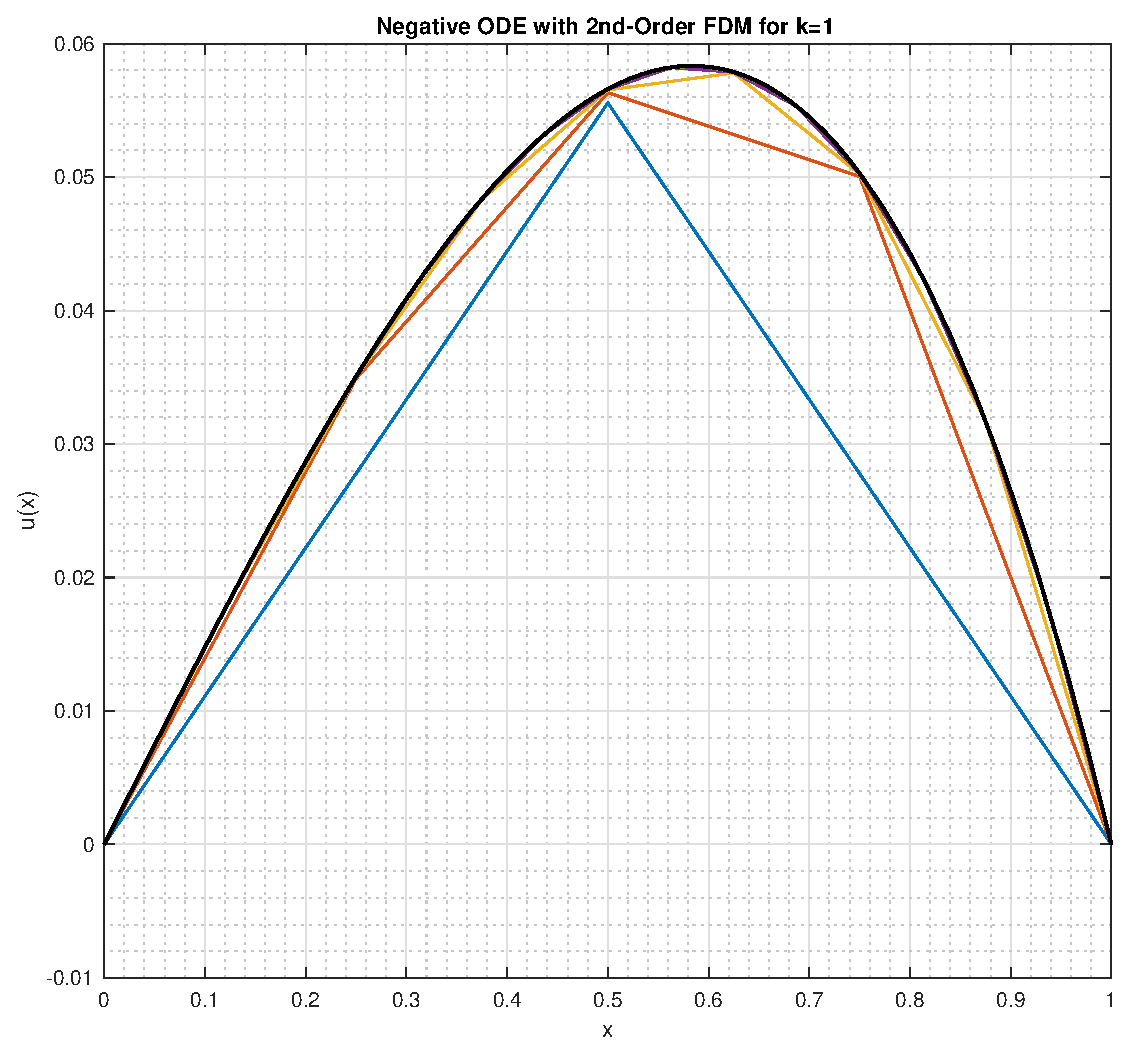
\includegraphics[width = 0.49\linewidth]{negative_ode_order_2_k_1}
		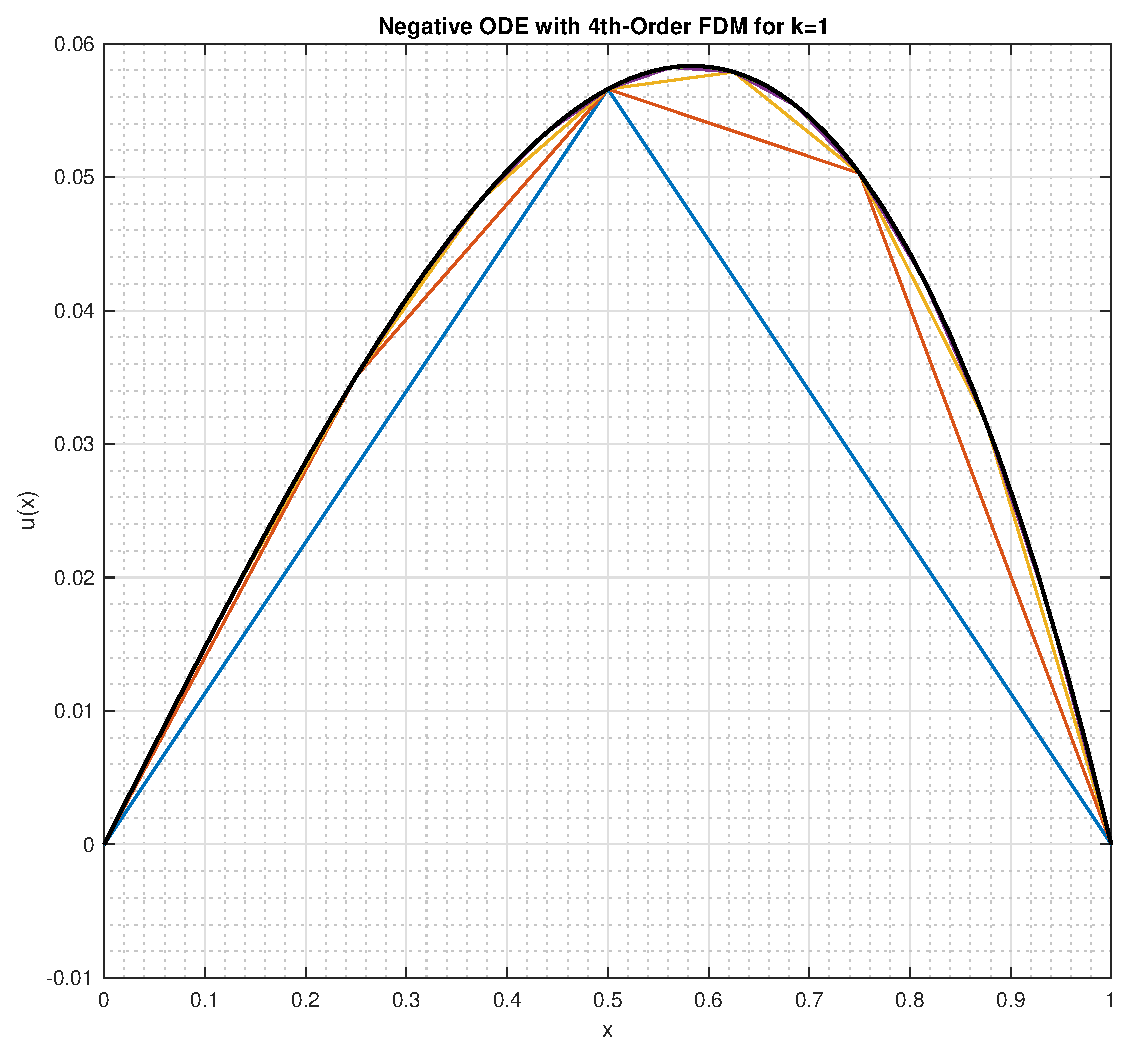
\includegraphics[width = 0.49\linewidth]{negative_ode_order_4_k_1}
		\caption{Negative ODE -- 2nd-Order and 4th-Order FDM for $k = 1$}
	\end{center}
\end{figure}

\begin{figure}[H]
	\begin{center}
		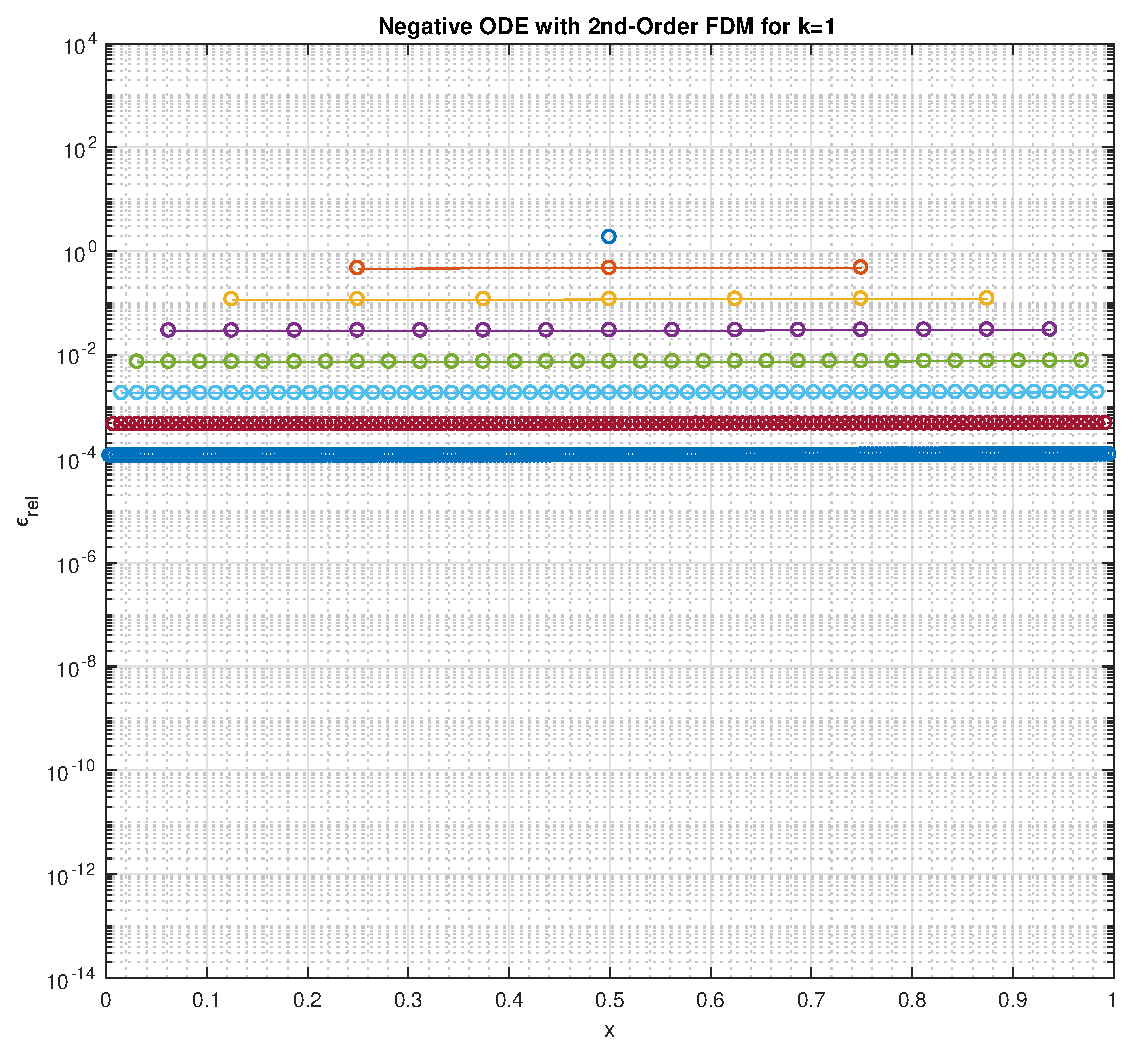
\includegraphics[width = 0.49\linewidth]{error_negative_ode_order_2_k_1}
		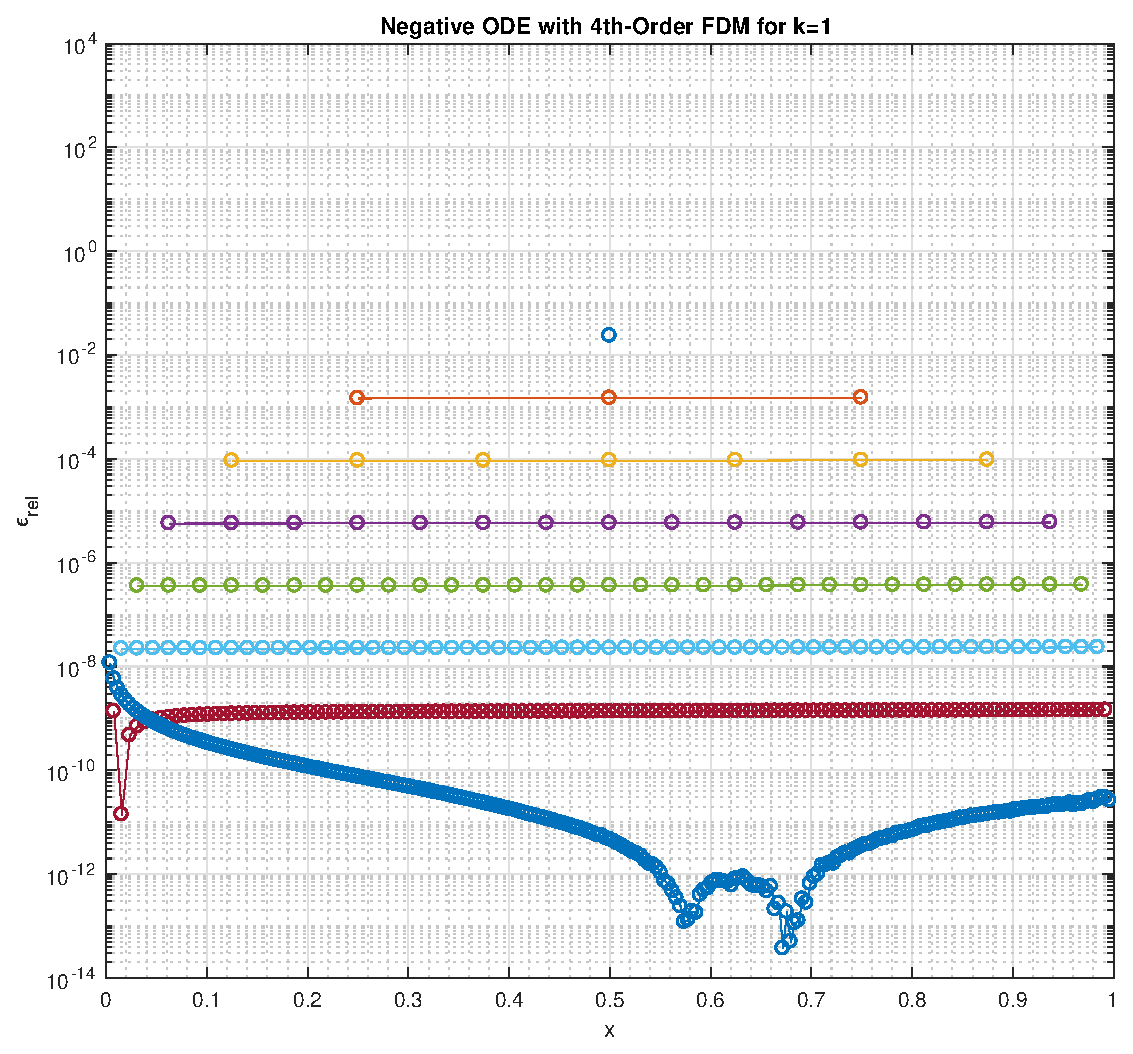
\includegraphics[width = 0.49\linewidth]{error_negative_ode_order_4_k_1}
		\caption{Pointwise Error -- Negative ODE -- 2nd-Order and 4th-Order FDM for $k = 1$}
	\end{center}
\end{figure}

\begin{center}
	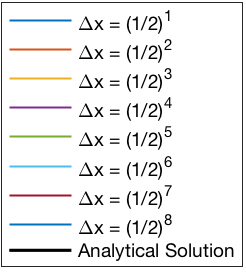
\includegraphics[height = 0.13\linewidth]{legend}
\end{center}

\newpage

\begin{figure}[H]
	\begin{center}
		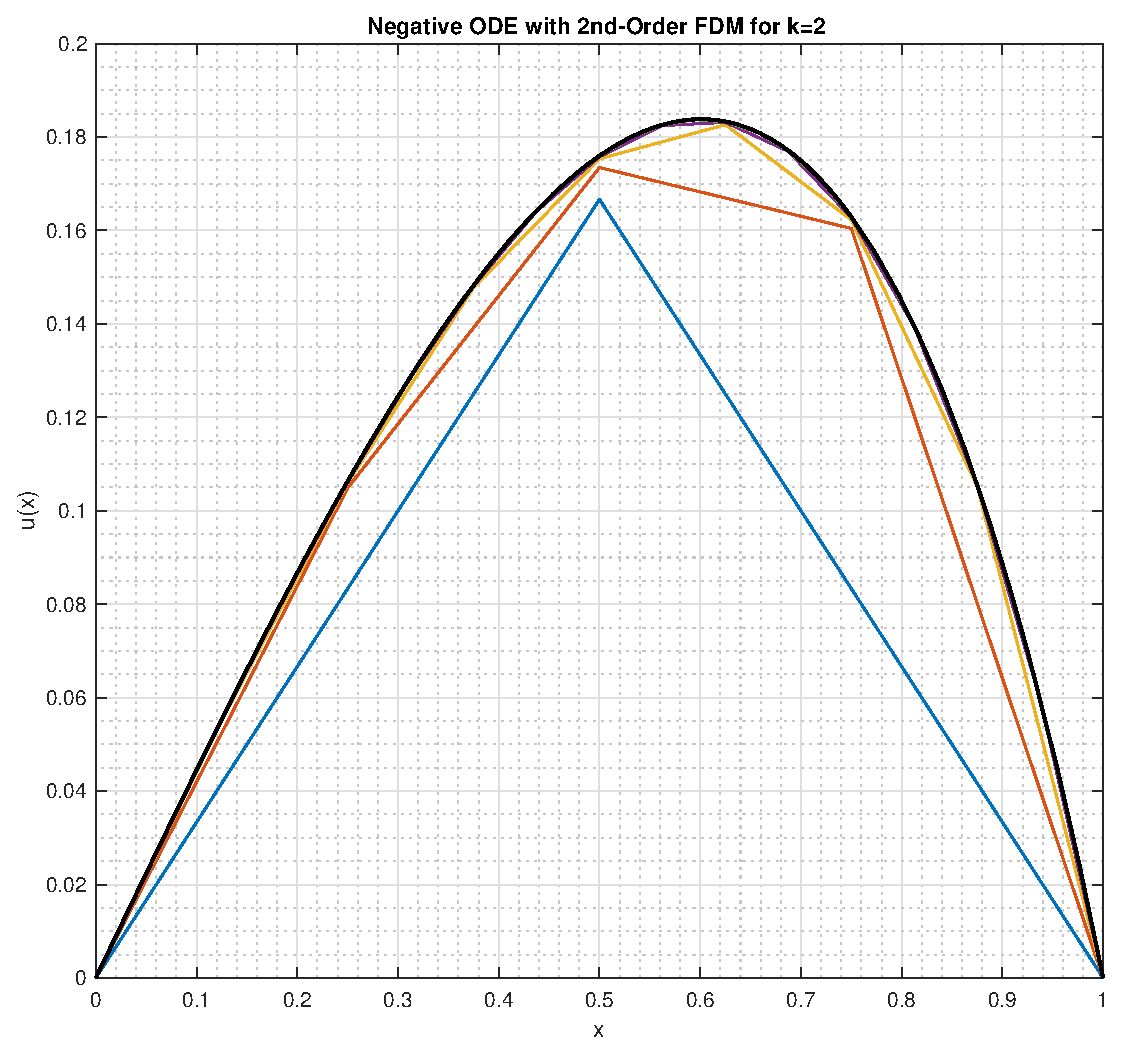
\includegraphics[width = 0.49\linewidth]{negative_ode_order_2_k_2}
		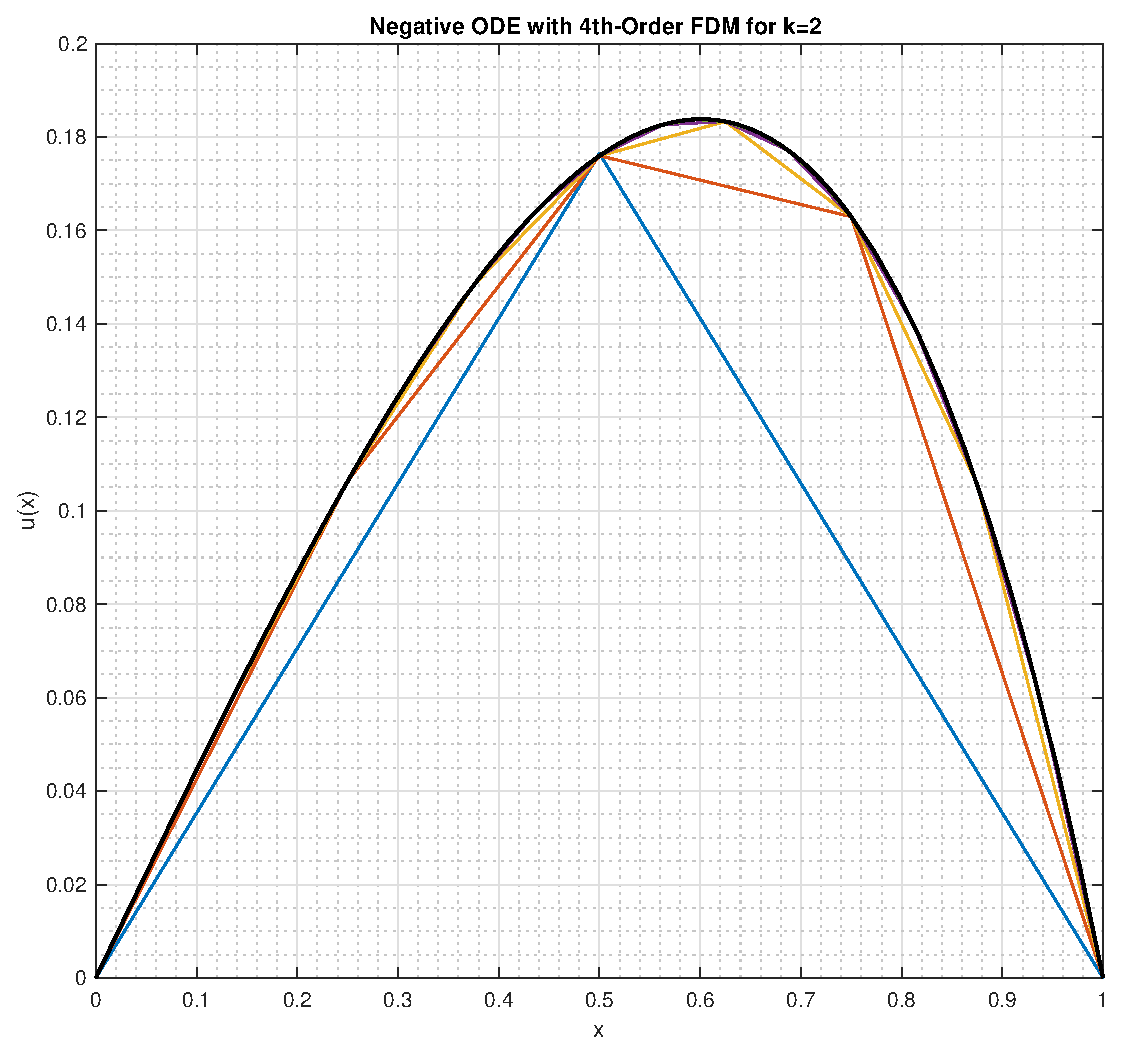
\includegraphics[width = 0.49\linewidth]{negative_ode_order_4_k_2}
		\caption{Negative ODE -- 2nd-Order and 4th-Order FDM for $k = 2$}
	\end{center}
\end{figure}

\begin{figure}[H]
	\begin{center}
		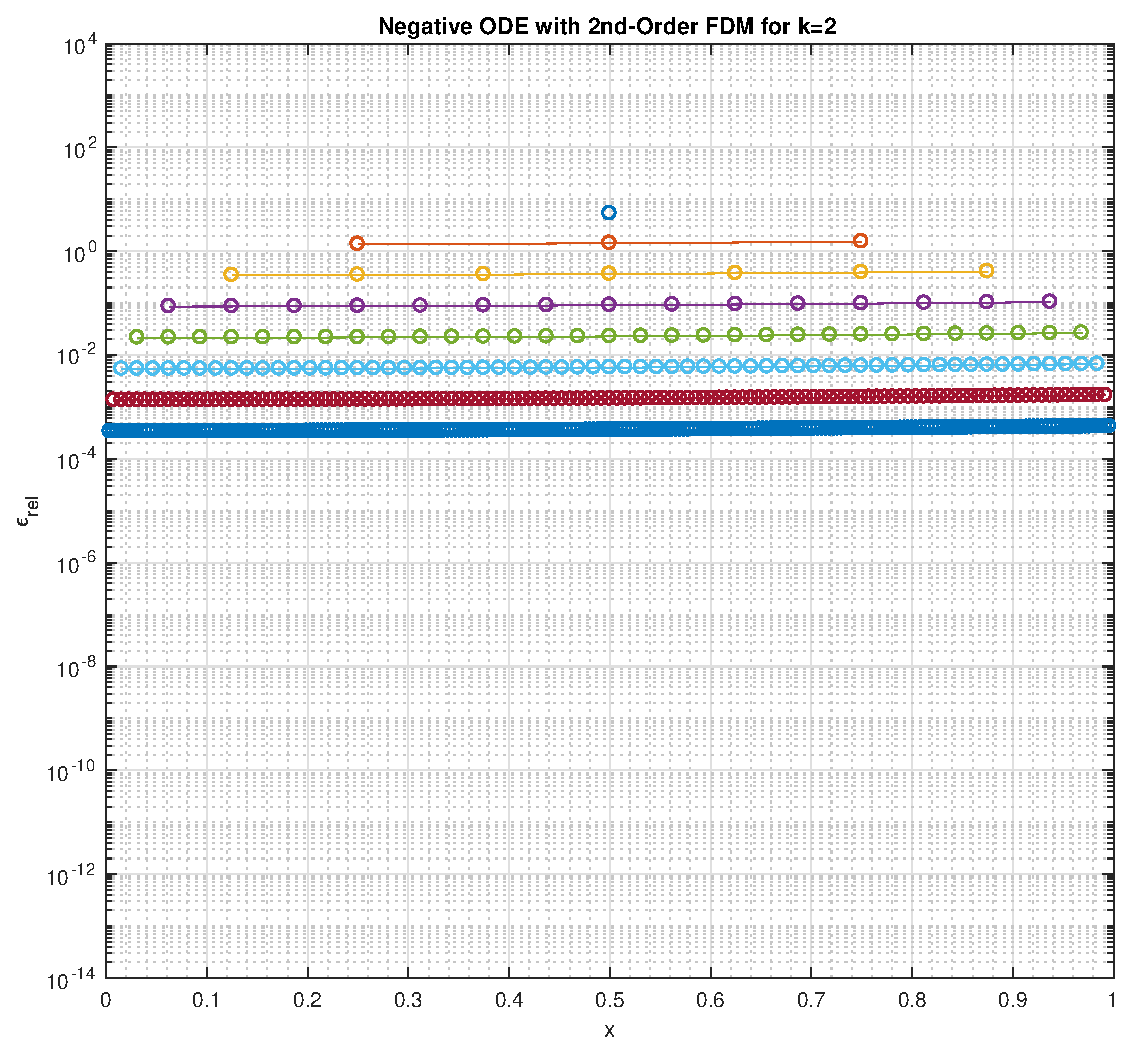
\includegraphics[width = 0.49\linewidth]{error_negative_ode_order_2_k_2}
		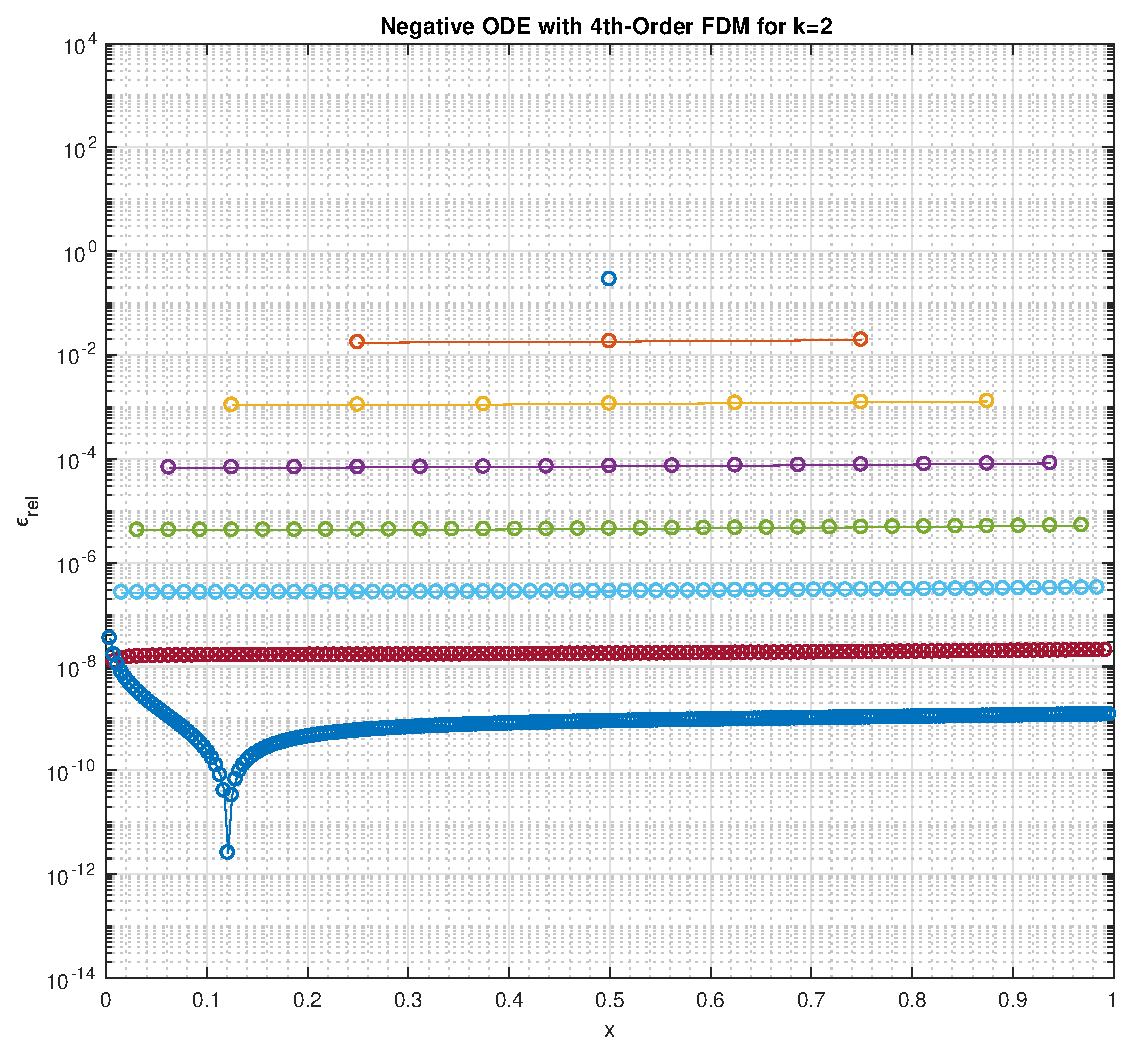
\includegraphics[width = 0.49\linewidth]{error_negative_ode_order_4_k_2}
		\caption{Pointwise Error -- Negative ODE -- 2nd-Order and 4th-Order FDM for $k = 2$}
	\end{center}
\end{figure}

\begin{center}
	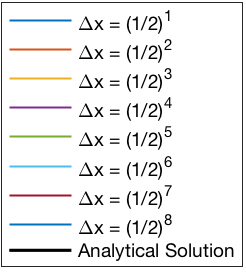
\includegraphics[height = 0.25\linewidth]{legend}
\end{center}

\newpage

\begin{figure}[H]
	\begin{center}
		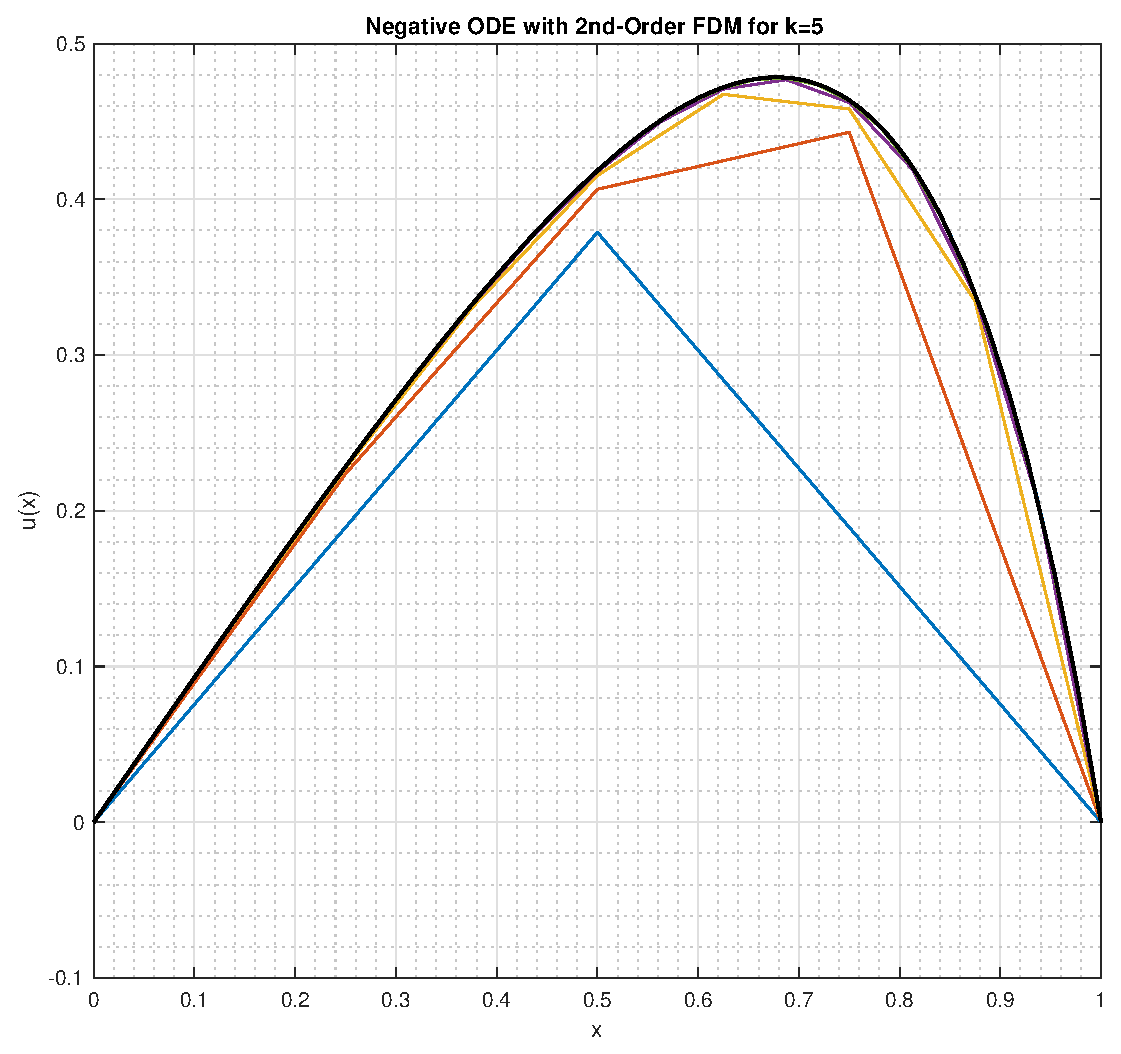
\includegraphics[width = 0.49\linewidth]{negative_ode_order_2_k_5}
		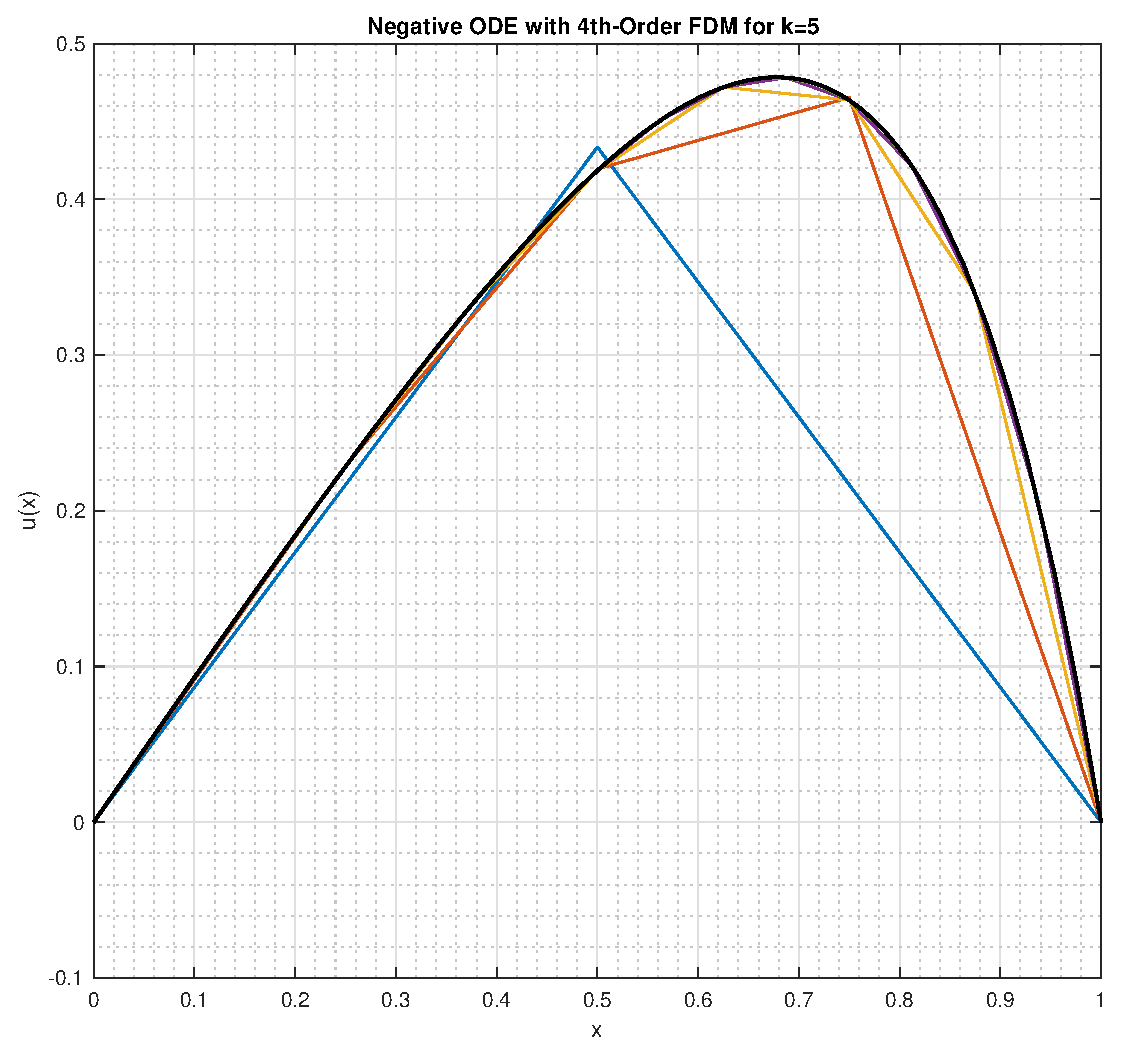
\includegraphics[width = 0.49\linewidth]{negative_ode_order_4_k_5}
		\caption{Negative ODE -- 2nd-Order and 4th-Order FDM for $k = 5$}
	\end{center}
\end{figure}

\begin{figure}[H]
	\begin{center}
		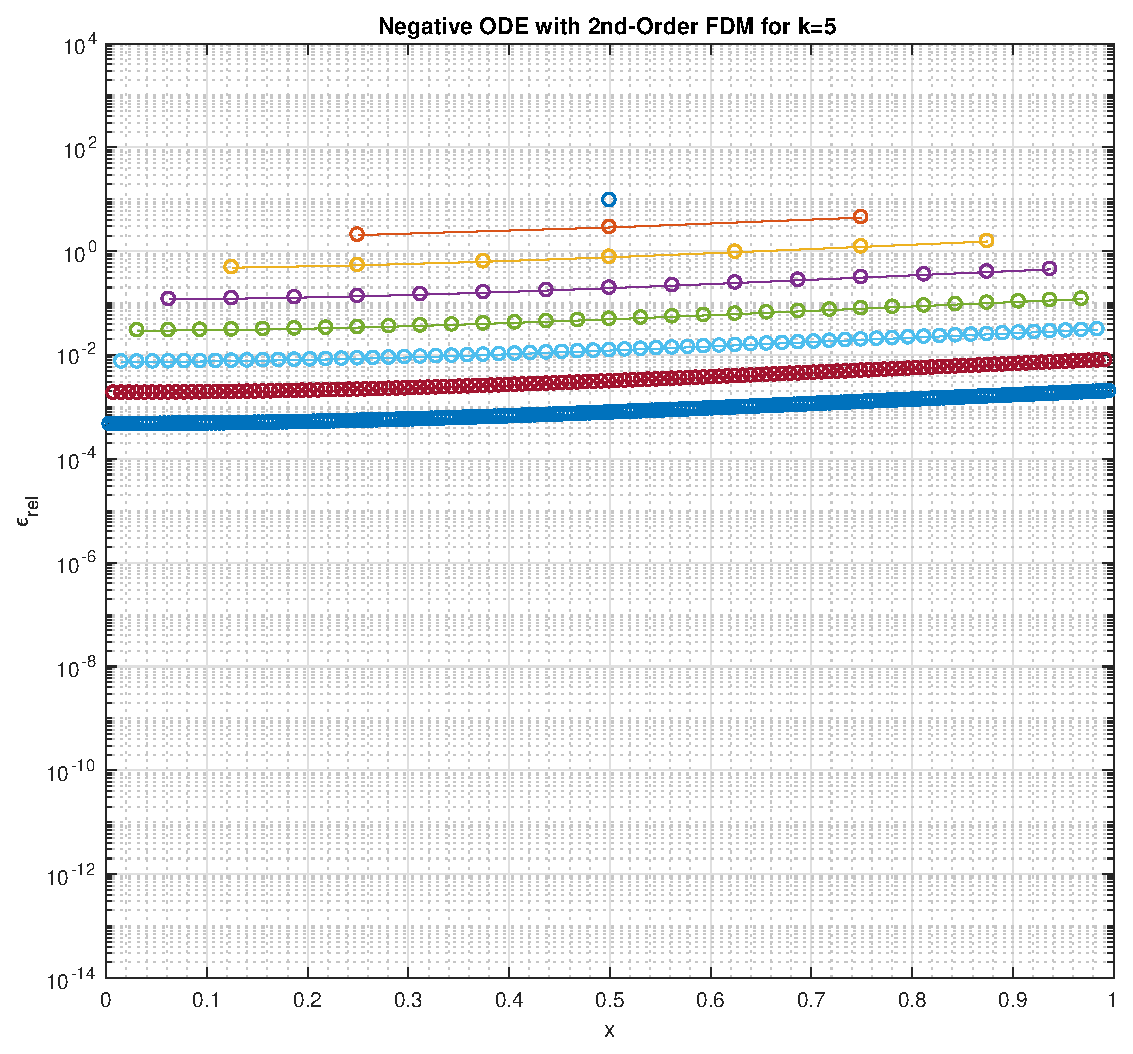
\includegraphics[width = 0.49\linewidth]{error_negative_ode_order_2_k_5}
		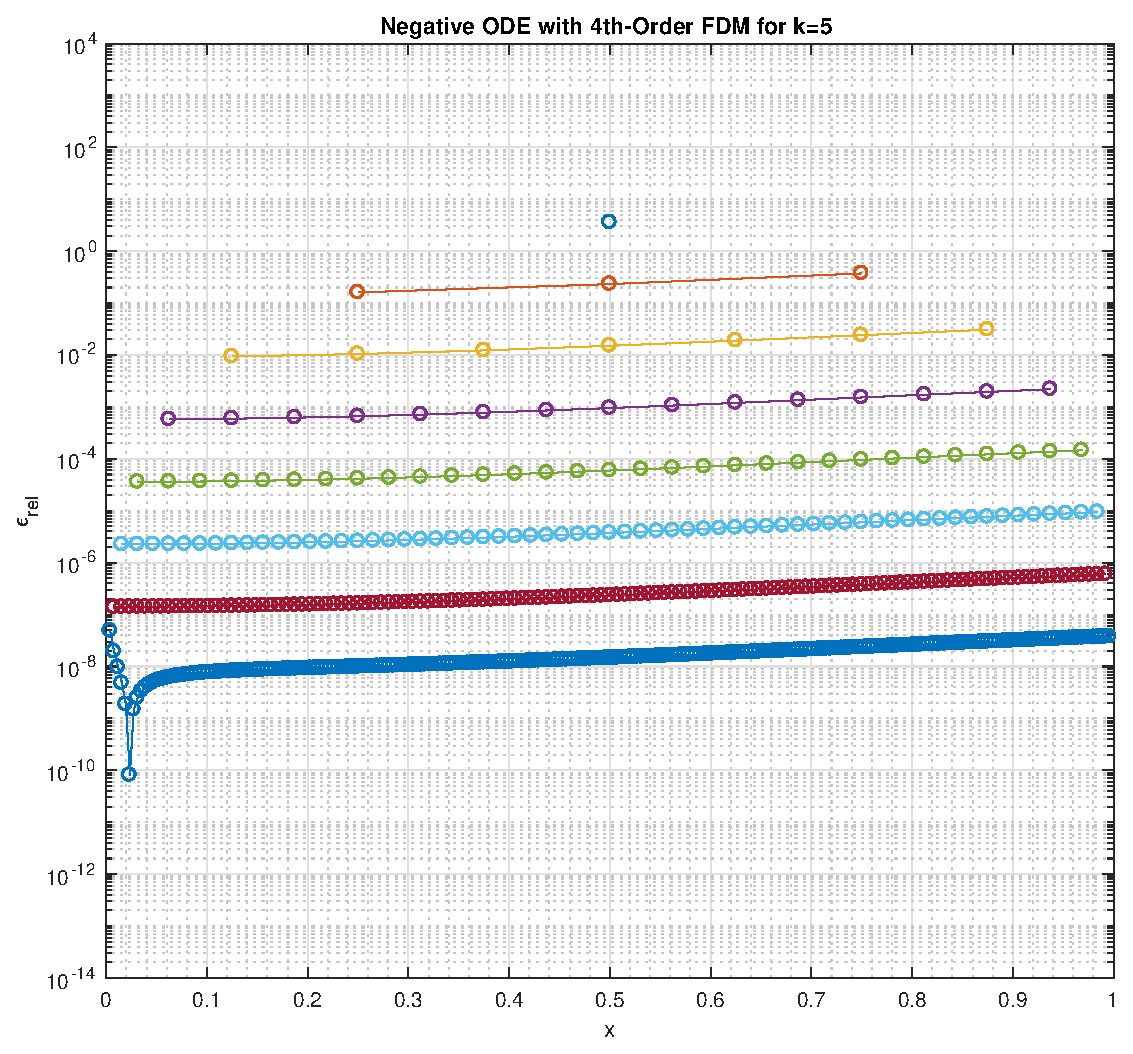
\includegraphics[width = 0.49\linewidth]{error_negative_ode_order_4_k_5}
		\caption{Pointwise Error -- Negative ODE -- 2nd-Order and 4th-Order FDM for $k = 5$}
	\end{center}
\end{figure}

\begin{center}
	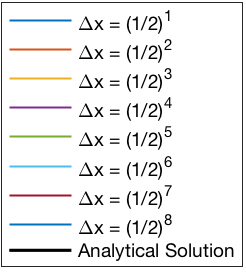
\includegraphics[height = 0.25\linewidth]{legend}
\end{center}

\newpage

\begin{figure}[H]
	\begin{center}
		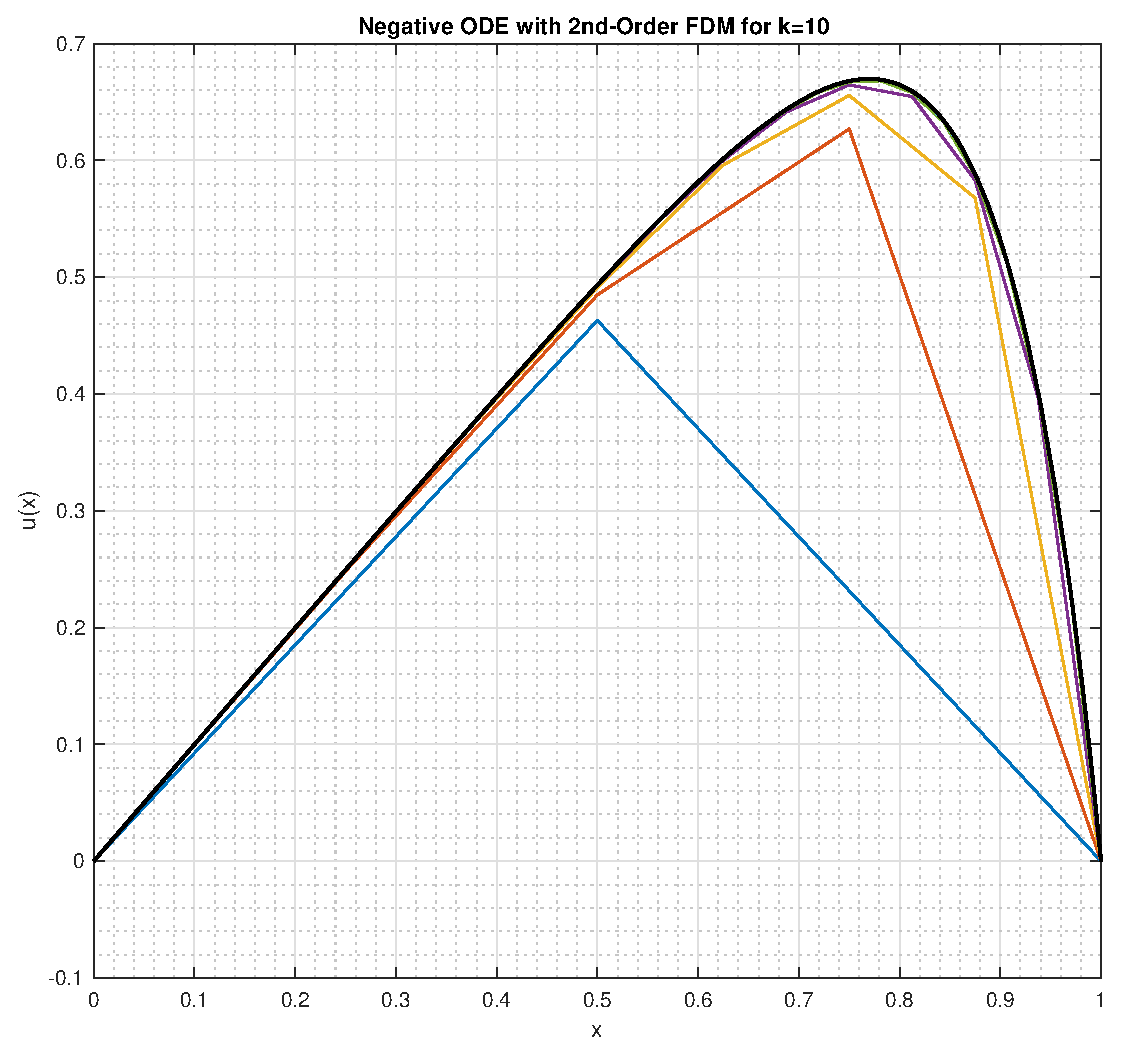
\includegraphics[width = 0.49\linewidth]{negative_ode_order_2_k_10}
		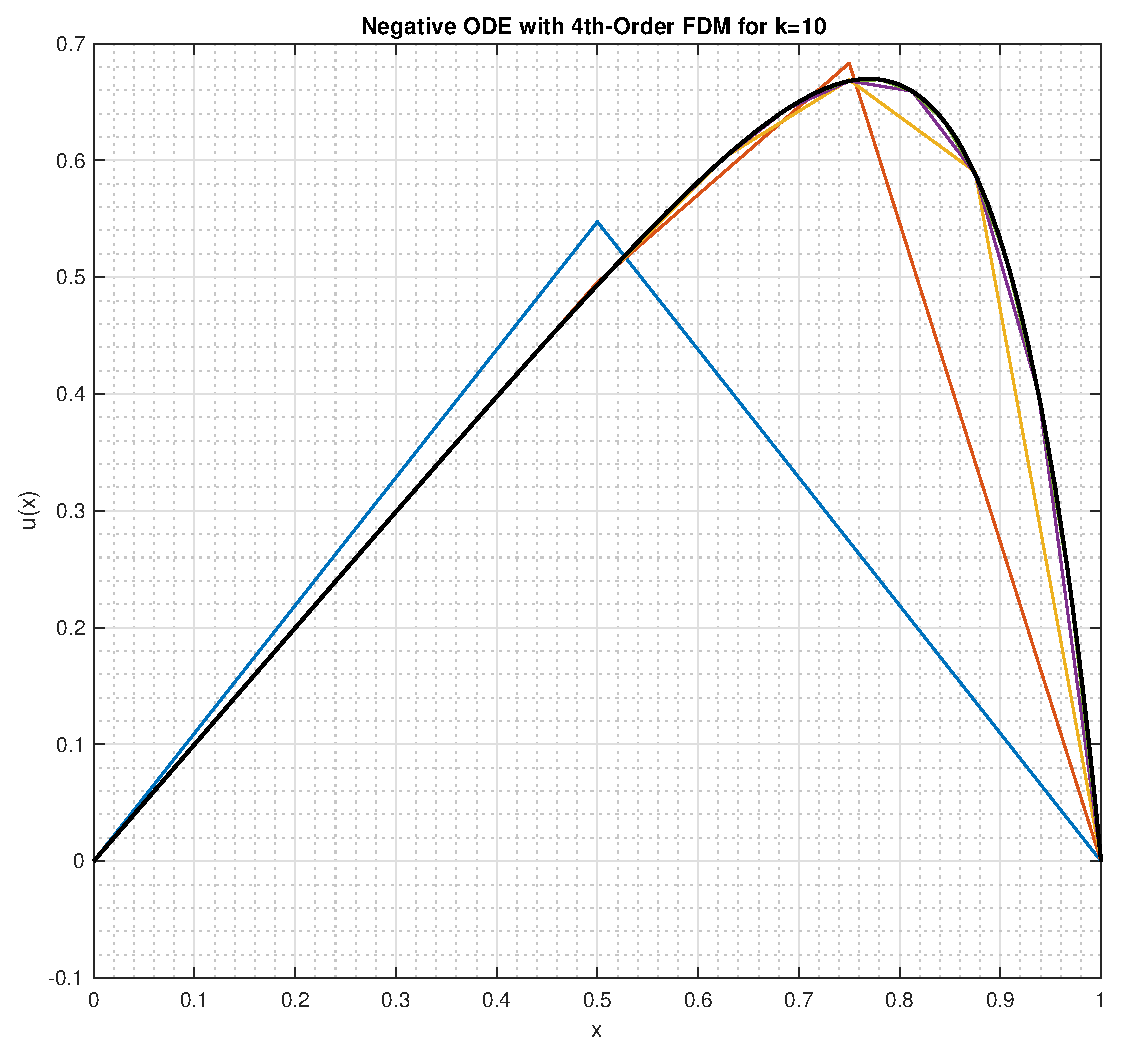
\includegraphics[width = 0.49\linewidth]{negative_ode_order_4_k_10}
		\caption{Negative ODE -- 2nd-Order and 4th-Order FDM for $k = 10$}
	\end{center}
\end{figure}

\begin{figure}[H]
	\begin{center}
		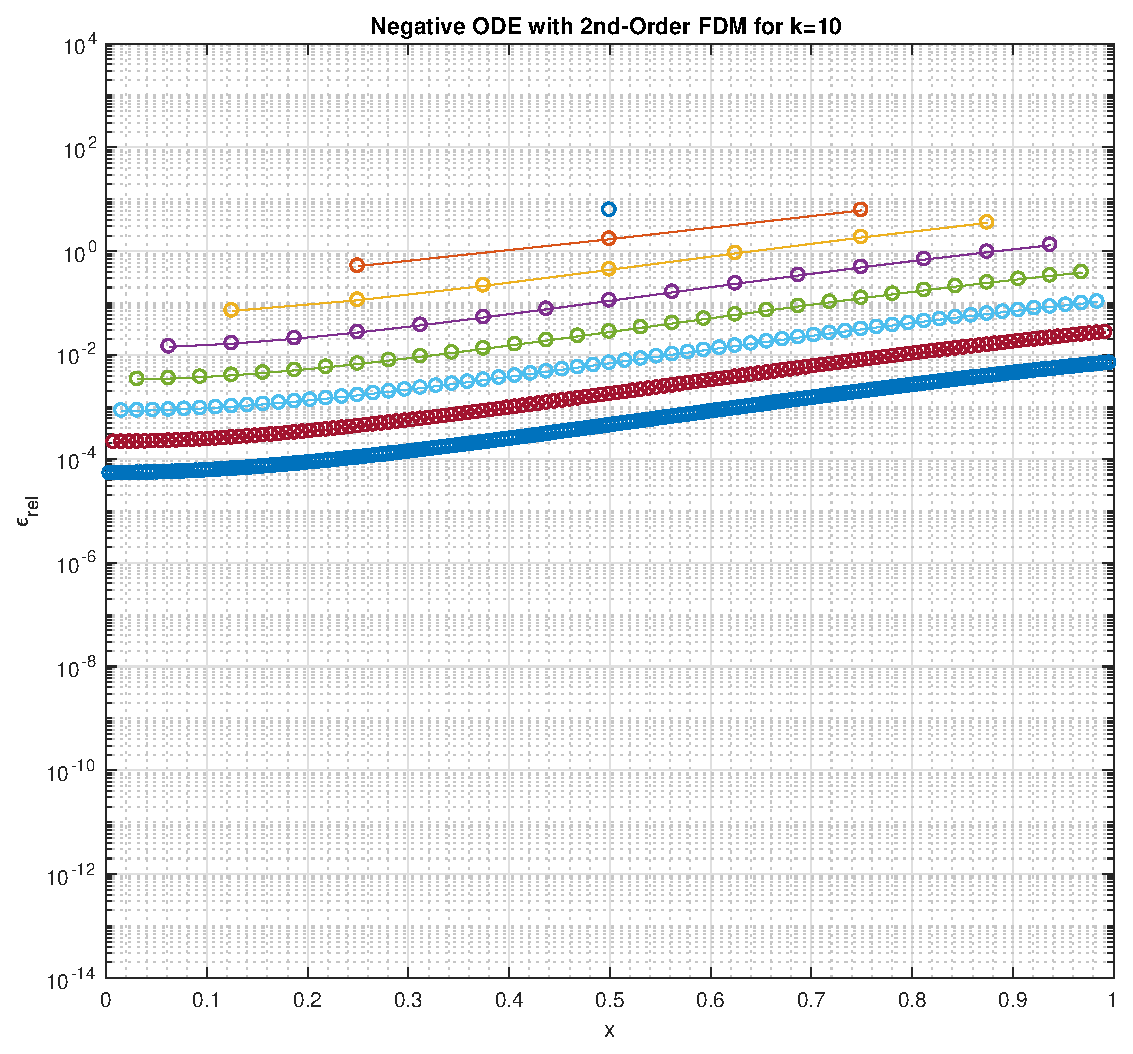
\includegraphics[width = 0.49\linewidth]{error_negative_ode_order_2_k_10}
		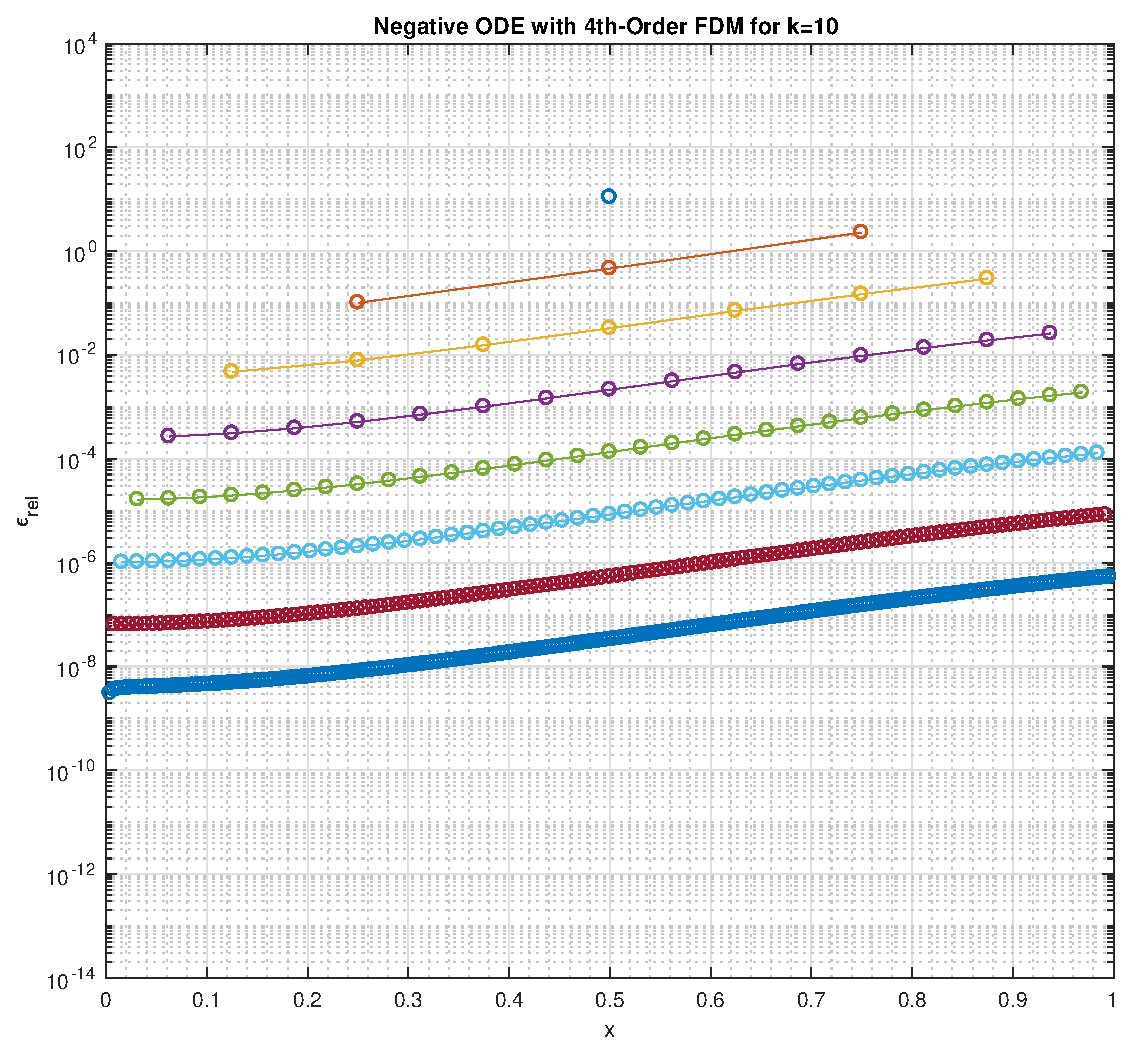
\includegraphics[width = 0.49\linewidth]{error_negative_ode_order_4_k_10}
		\caption{Pointwise Error -- Negative ODE -- 2nd-Order and 4th-Order FDM for $k = 10$}
	\end{center}
\end{figure}

\begin{center}
	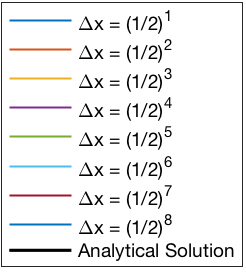
\includegraphics[height = 0.25\linewidth]{legend}
\end{center}

\newpage

\begin{figure}[H]
	\begin{center}
		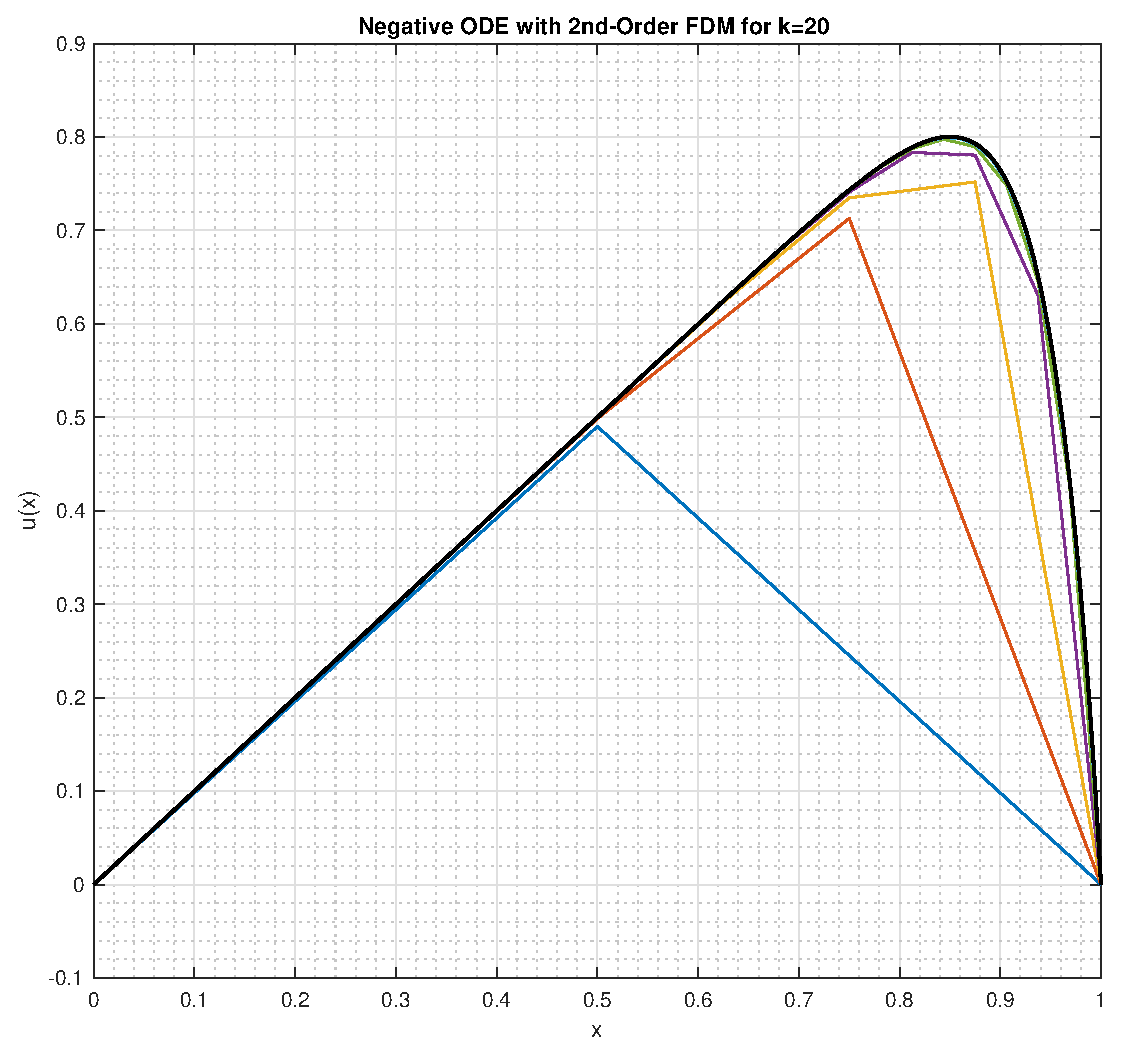
\includegraphics[width = 0.49\linewidth]{negative_ode_order_2_k_20}
		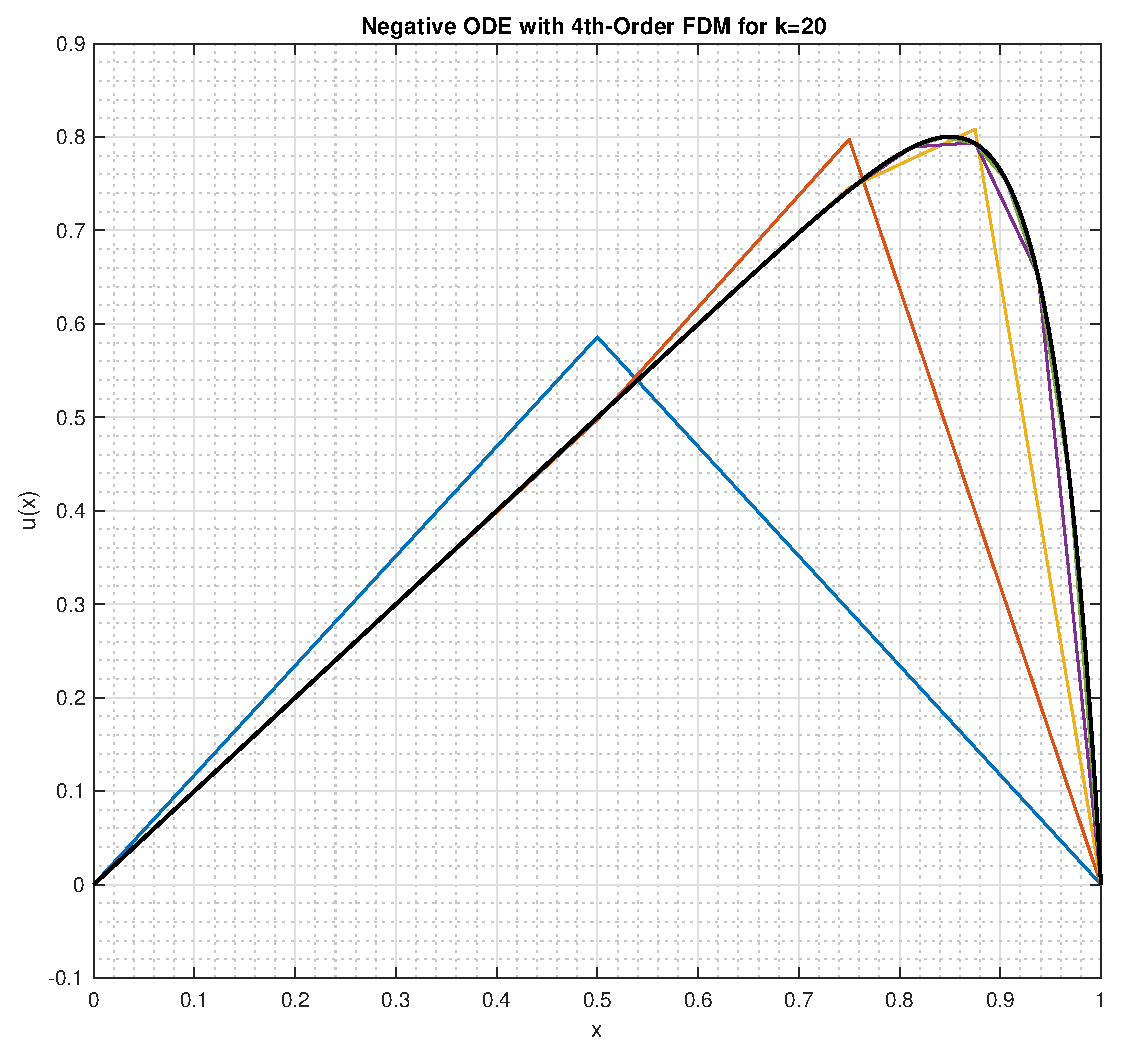
\includegraphics[width = 0.49\linewidth]{negative_ode_order_4_k_20}
		\caption{Negative ODE -- 2nd-Order and 4th-Order FDM for $k = 20$}
	\end{center}
\end{figure}

\begin{figure}[H]
	\begin{center}
		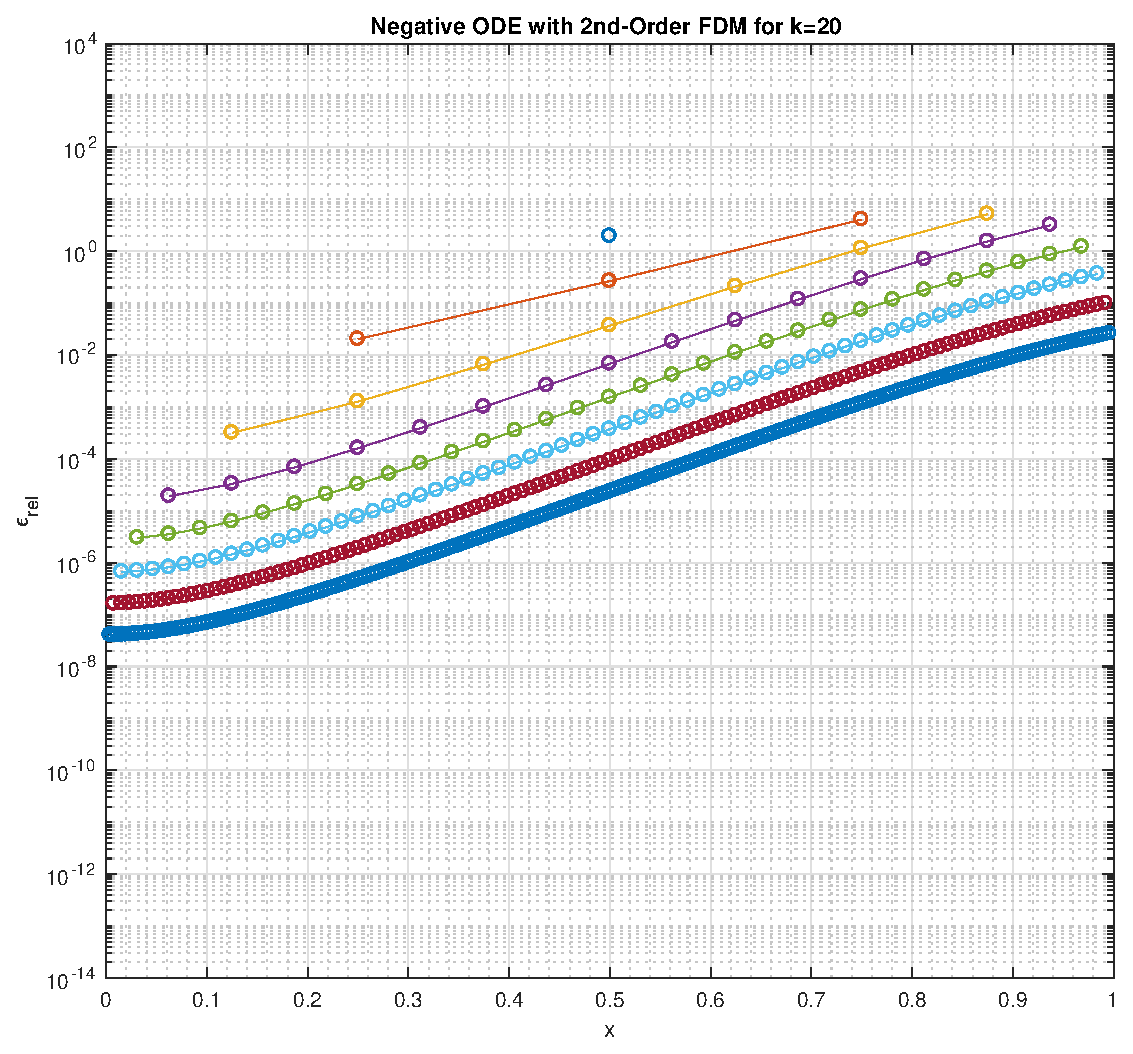
\includegraphics[width = 0.49\linewidth]{error_negative_ode_order_2_k_20}
		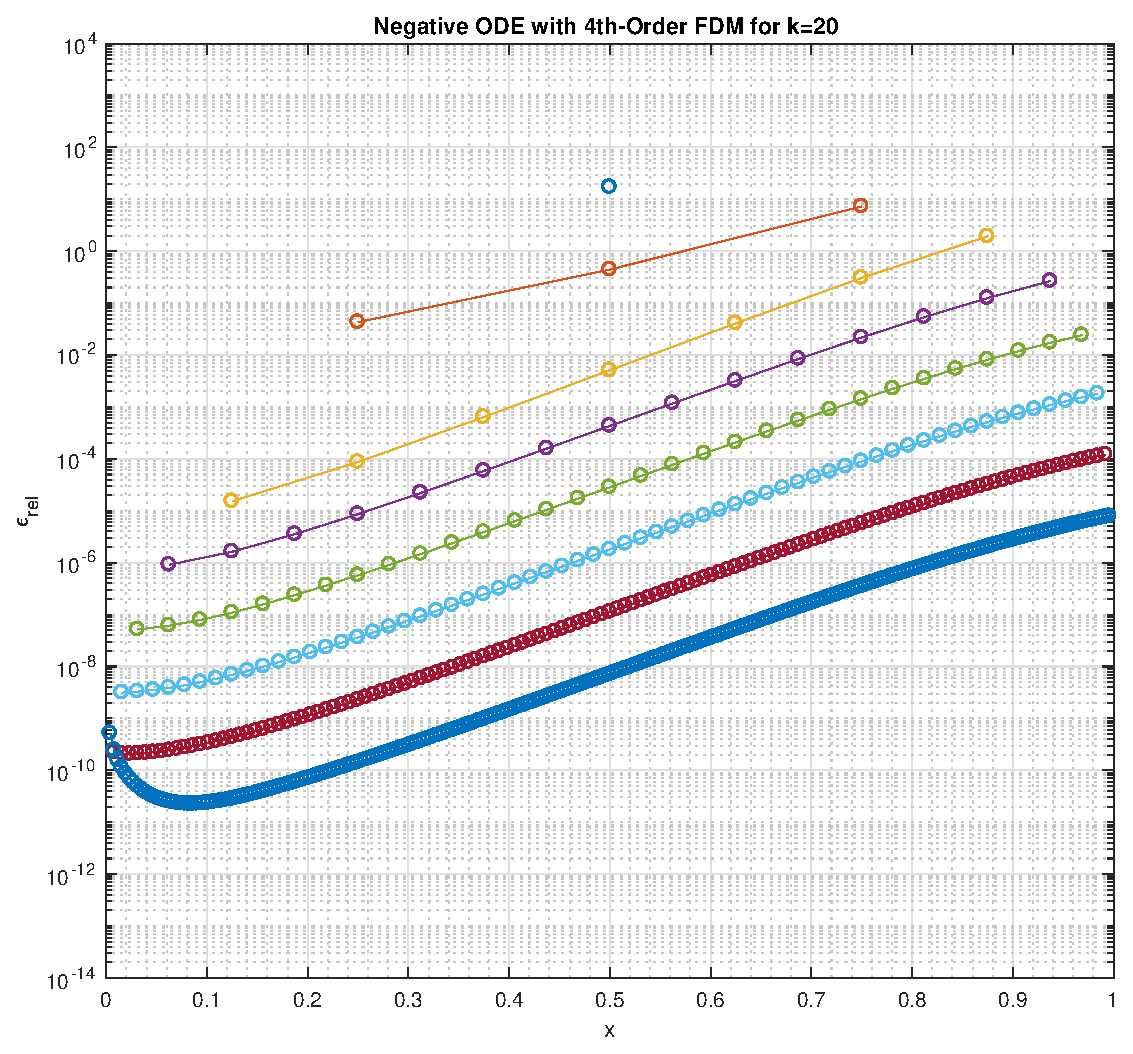
\includegraphics[width = 0.49\linewidth]{error_negative_ode_order_4_k_20}
		\caption{Pointwise Error -- Negative ODE -- 2nd-Order and 4th-Order FDM for $k = 20$}
	\end{center}
\end{figure}

\begin{center}
	\includegraphics[height = 0.25\linewidth]{legend}
\end{center}

\newpage

\subsection{Discussion}

Meshes were calculated for $\Delta x = 0.5^{18}$, but only meshes up to $\Delta x = 0.5^8$ are shown in the tables and figures due to sheer size and readability.

For the positive ODE, the analytical solution oscillates and generally increases in the amplitude of the oscillations as $k$ increases. Like expected, as mesh size is decreased, the approximation of the solution to the model problem approaches the analytical solution. The fourth-order methods demonstrate quicker error reduction than second-order methods.

For the negative ODE, the analytical solution asymptotically approaches the line $y = x$ as $k$ increases. Like expected, as mesh size is decreased, the approximation of the solution to the model problem approaches the analytical solution. Unlike the positive ODE, at high values of $k$ ($k \ge 20$), the mesh size $\Delta x = (1/2)^6$ is sufficient to resolve the solution as difference between different values of $k$ is increasingly negligible. The fourth-order methods demonstrate quicker error reduction than second-order methods.

\newpage

\section{Convergence Analysis}

\subsection{Rate of Convergence Derivation}

Let the error for a particular mesh size $\Delta x$ be $E\left(\Delta x\right)$:
\begin{equation}
E\left(\Delta x\right) = C\left(\Delta x\right)^\beta
\end{equation}
Then for a smaller mesh size $\frac{\Delta x}{2}$ we have:
\begin{equation}
E\left(\frac{\Delta x}{2}\right) = C\left(\frac{\Delta x}{2}\right)^\beta
\end{equation}
Dividing the error at each mesh size and taking the logarithm:
\begin{equation}
\frac{E\left(\Delta x\right)}{E\left(\frac{\Delta x}{2}\right)} = \frac{C\left(\Delta x\right)^\beta}{C\left(\frac{\Delta x}{2}\right)^\beta} = 2^\beta
\end{equation}
\begin{equation}
\log\left[\frac{E\left(\Delta x\right)}{E\left(\frac{\Delta x}{2}\right)}\right] = \log(2^\beta)
\end{equation}
\begin{equation}
\log\left[\frac{E\left(\Delta x\right)}{E\left(\frac{\Delta x}{2}\right)}\right] = \beta \log(2)
\end{equation}
Rearranging for $\beta$ and simplifying:
\begin{equation}
\beta = \frac{1}{\log(2)} \left[\log\left(E\left(\Delta x\right)\right) - \log\left(E\left(\frac{\Delta x}{2}\right)\right)\right] 
\end{equation}
Denoting $E^*_{\Delta x} = \log\left(E\left(\Delta x\right)\right)$:
\begin{equation}
\mathbf{\beta = \frac{E^*_{\Delta x} - E^*_{\frac{\Delta x}{2}}}{\log (2)}}
\end{equation}

\subsection{First-Order First-Derivative Finite Difference Method}

\subsubsection{Derivation}

Developing the Taylor series for $u(x)$ in the vicinity of $x = 1$:
\begin{equation}
u_{N-1} = u_N - \Delta x u'_N + \frac{\Delta x^2}{2} u''_N + \mathcal{O}(\Delta x^3)
\end{equation}
Rearranging terms to solve for $u'_N$:
\begin{equation}
u'_N = \frac{u_N - u_{N-1}}{\Delta x} + \mathcal{O}(\Delta x)
\end{equation}
Switching to a compact notation where $u_N = u_N$, $u_{N-1} = u_{N-1}$, etc.:
\begin{equation}
u'_N = \frac{u_N - u_{N-1}}{\Delta x} + \mathcal{O}(\Delta x)
\end{equation}
Applying the boundary condition $u(1) = u_N = 0$:
\begin{equation}
u'_N = \frac{- u_{N-1}}{\Delta x} + \mathcal{O}(\Delta x)
\end{equation}

From this specific first-derivative formulation at the boundary $x = 1$ using the finite difference method, the approximation can be observed to be first-order ($\mathcal{O}(\Delta x)$).

\newpage

\subsubsection{Results}

\begin{figure}[H]
	\begin{center}
		\includegraphics[width = 0.76\linewidth]{positive_ode_order_2_fd_order_1}
		\caption{Positive ODE -- 2nd-Order FDM with 1st-Order First-Derivative Approximation}	
	\end{center}
\end{figure}

\vfill

\begin{table}[H]
	\begin{tabular}{|c|c|c|c|c|c|}
\hline
\textbf{$\Delta x$}&\textbf{$\beta(k=1)$}&\textbf{$\beta(k=2)$}&\textbf{$\beta(k=5)$}&\textbf{$\beta(k=10)$}&\textbf{$\beta(k=20)$}\\\hline
0.5000&0.8869&0.9362&1.5051&0.3555&0.5380\\\hline
0.2500&0.9469&0.9678&0.2328&0.4475&2.1685\\\hline
0.1250&0.9742&0.9841&0.7828&1.9264&-5.0349\\\hline
0.0625&0.9873&0.9921&0.9053&4.6303&4.8880\\\hline
0.0312&0.9937&0.9961&0.9552&-2.2852&0.0549\\\hline
0.0156&0.9969&0.9980&0.9781&0.4326&0.1039\\\hline
0.0078&0.9984&0.9990&0.9892&0.7790&0.6880\\\hline
0.0039&0.9992&0.9995&0.9946&0.9006&0.8647\\\hline
0.0020&0.9996&0.9998&0.9973&0.9527&0.9366\\\hline
0.0010&0.9998&0.9999&0.9987&0.9769&0.9693\\\hline
0.0005&0.9999&0.9999&0.9993&0.9886&0.9849\\\hline
0.0002&1.0000&1.0000&0.9997&0.9943&0.9925\\\hline
0.0001&1.0000&1.0000&0.9998&0.9972&0.9963\\\hline
0.0001&1.0000&1.0000&0.9999&0.9986&0.9981\\\hline
0.0000&1.0000&1.0000&0.9997&0.9991&0.9991\\\hline
0.0000&1.0000&1.0000&0.9982&0.9981&0.9994\\\hline
0.0000&1.0001&0.9999&0.9861&0.9868&0.9987\\\hline
\end{tabular}

	\caption{Positive ODE -- 2nd-Order FDM with 1st-Order First-Derivative Approximation -- Rate of Convergence Values}	
\end{table}\begin{figure}[H]
	
	\begin{center}
		\includegraphics[width = 0.76\linewidth]{negative_ode_order_2_fd_order_1}
		\caption{Negative ODE -- 2nd-Order FDM with 1st-Order First-Derivative Approximation}	
	\end{center}
\end{figure}

\vfill

\begin{table}[H]
	\begin{tabular}{|c|c|c|c|c|c|}
\hline
\textbf{$\Delta x$}&\textbf{$\beta(k=1)$}&\textbf{$\beta(k=2)$}&\textbf{$\beta(k=5)$}&\textbf{$\beta(k=10)$}&\textbf{$\beta(k=20)$}\\\hline
0.5000&0.8389&0.7760&0.5413&0.3146&0.1582\\\hline
0.2500&0.9248&0.8934&0.7511&0.5425&0.3146\\\hline
0.1250&0.9637&0.9486&0.8777&0.7513&0.5425\\\hline
0.0625&0.9822&0.9749&0.9408&0.8777&0.7513\\\hline
0.0312&0.9912&0.9876&0.9710&0.9408&0.8777\\\hline
0.0156&0.9956&0.9938&0.9857&0.9710&0.9408\\\hline
0.0078&0.9978&0.9969&0.9929&0.9857&0.9710\\\hline
0.0039&0.9989&0.9985&0.9965&0.9929&0.9857\\\hline
0.0020&0.9995&0.9992&0.9982&0.9965&0.9929\\\hline
0.0010&0.9997&0.9996&0.9991&0.9982&0.9965\\\hline
0.0005&0.9999&0.9998&0.9996&0.9991&0.9982\\\hline
0.0002&0.9999&0.9999&0.9998&0.9996&0.9991\\\hline
0.0001&1.0000&1.0000&0.9999&0.9998&0.9996\\\hline
0.0001&1.0000&1.0000&0.9999&0.9999&0.9998\\\hline
0.0000&1.0000&1.0000&0.9999&0.9999&0.9999\\\hline
0.0000&1.0000&1.0000&0.9997&0.9999&0.9999\\\hline
0.0000&1.0000&0.9999&0.9976&0.9996&0.9999\\\hline
\end{tabular}

	\caption{Negative ODE -- 2nd-Order FDM with 1st-Order First-Derivative Approximation -- Rate of Convergence Values}	
\end{table}

\begin{figure}[H]
	\begin{center}
		\includegraphics[width = 0.76\linewidth]{positive_ode_order_4_fd_order_1}
		\caption{Positive ODE -- 4th-Order FDM with 1st-Order First-Derivative Approximation}	
	\end{center}
\end{figure}

\vfill

\begin{table}[H]
	\begin{tabular}{|c|c|c|c|c|c|}
\hline
\textbf{$\Delta x$}&\textbf{$\beta(k=1)$}&\textbf{$\beta(k=2)$}&\textbf{$\beta(k=5)$}&\textbf{$\beta(k=10)$}&\textbf{$\beta(k=20)$}\\\hline
0.5000&0.8919&1.0064&0.5598&0.5812&0.6533\\\hline
0.2500&0.9540&1.0288&0.9093&4.0424&-0.1659\\\hline
0.1250&0.9789&1.0210&1.0021&-1.8716&-0.5465\\\hline
0.0625&0.9899&1.0121&1.0122&0.5875&0.3887\\\hline
0.0312&0.9951&1.0065&1.0087&0.8523&0.8581\\\hline
0.0156&0.9976&1.0033&1.0050&0.9353&0.9523\\\hline
0.0078&0.9988&1.0017&1.0026&0.9695&0.9802\\\hline
0.0039&0.9994&1.0009&1.0014&0.9851&0.9909\\\hline
0.0020&0.9997&1.0004&1.0007&0.9927&0.9956\\\hline
0.0010&0.9998&1.0002&1.0003&0.9964&0.9979\\\hline
0.0005&0.9999&1.0001&1.0002&0.9982&0.9989\\\hline
0.0002&1.0000&1.0000&1.0001&0.9991&0.9995\\\hline
0.0001&0.9999&0.9999&1.0000&0.9995&0.9997\\\hline
0.0001&0.9995&0.9988&1.0001&0.9997&0.9999\\\hline
0.0000&0.9957&0.9906&1.0002&1.0002&0.9999\\\hline
0.0000&0.9662&0.9267&1.0013&1.0012&1.0002\\\hline
0.0000&0.7549&0.5175&1.0106&1.0091&1.0008\\\hline
\end{tabular}

	\caption{Positive ODE -- 4th-Order FDM with 1st-Order First-Derivative Approximation -- Rate of Convergence Values}	
\end{table}

\begin{figure}[H]
	\begin{center}
		\includegraphics[width = 0.76\linewidth]{negative_ode_order_4_fd_order_1}
		\caption{Negative ODE -- 4th-Order FDM with 1st-Order First-Derivative Approximation}	
	\end{center}
\end{figure}

\vfill

\begin{table}[H]
	\begin{tabular}{|c|c|c|c|c|c|}
\hline
\textbf{$\Delta x$}&\textbf{$\beta(k=1)$}&\textbf{$\beta(k=2)$}&\textbf{$\beta(k=5)$}&\textbf{$\beta(k=10)$}&\textbf{$\beta(k=20)$}\\\hline
0.5000&0.8362&0.7712&0.5508&0.3350&0.1733\\\hline
0.2500&0.9199&0.8809&0.7394&0.5508&0.3350\\\hline
0.1250&0.9603&0.9391&0.8603&0.7394&0.5508\\\hline
0.0625&0.9802&0.9692&0.9276&0.8603&0.7394\\\hline
0.0312&0.9901&0.9845&0.9631&0.9276&0.8603\\\hline
0.0156&0.9951&0.9922&0.9814&0.9631&0.9276\\\hline
0.0078&0.9975&0.9961&0.9907&0.9814&0.9631\\\hline
0.0039&0.9988&0.9981&0.9953&0.9907&0.9814\\\hline
0.0020&0.9994&0.9990&0.9977&0.9953&0.9907\\\hline
0.0010&0.9997&0.9995&0.9988&0.9977&0.9953\\\hline
0.0005&0.9998&0.9998&0.9994&0.9988&0.9977\\\hline
0.0002&0.9999&0.9999&0.9997&0.9994&0.9988\\\hline
0.0001&0.9999&0.9999&0.9999&0.9997&0.9994\\\hline
0.0001&0.9994&0.9996&0.9999&0.9999&0.9997\\\hline
0.0000&0.9956&0.9972&0.9999&0.9999&0.9998\\\hline
0.0000&0.9654&0.9778&0.9991&0.9998&0.9999\\\hline
0.0000&0.7496&0.8337&0.9930&0.9988&0.9997\\\hline
\end{tabular}

	\caption{Negative ODE -- 4th-Order FDM with 1st-Order First-Derivative Approximation -- Rate of Convergence Values}	
\end{table}

\newpage

\subsection{Second-Order First-Derivative Finite Difference Method}

\subsubsection{Derivation}

Developing the Taylor series for $u(x)$ in the vicinity of $x = 1$:
\begin{equation}
u_{N-1} = u_N - \Delta x u'_N + \frac{\Delta x^2}{2} u''_N + \mathcal{O}(\Delta x^3)
\end{equation}
Rearranging terms to solve for $u'_N$, but leaving the second-derivative term:
\begin{equation}
\label{eqn:2o1d}
u'_N = \frac{u_N - u_{N-1}}{\Delta x} + \frac{\Delta x}{2} u''_N + \mathcal{O}(\Delta x^2)
\end{equation}
Returning to the differential equation, rearranging for the second derivative, and evaluating the differential equation at $x = 1$ with corresponding boundary condition $u(1) = u_N = 0$:
\begin{equation}
\pm u''(x)+k^2u(x)=k^2x
\end{equation}
\begin{equation}
u''_N = \pm k^2(1-u_N)
\end{equation}
\begin{equation}
\label{eqn:2o2d}
u''_N = \pm k^2
\end{equation}
This equation yields the exact sign correspondence with the sign of the ODE.

Substituting Equation \ref{eqn:2o2d} into Equation \ref{eqn:2o1d}
\begin{equation}
u'_N = \frac{u_N - u_{N-1}}{\Delta x} \pm \frac{k^2 \Delta x}{2} + \mathcal{O}(\Delta x^2)
\end{equation}
Applying the boundary condition $u(1) = u_N = 0$:
\begin{equation}
u'_N = \frac{-u_{N-1}}{\Delta x} \pm \frac{k^2 \Delta x}{2} + \mathcal{O}(\Delta x^2)
\end{equation}

From this specific first-derivative formulation at the boundary $x = 1$ using the finite difference method, the approximation can be observed to be second-order ($\mathcal{O}(\Delta x^2)$).

\newpage

\subsubsection{Results}

\begin{figure}[H]
	\begin{center}
		\includegraphics[width = 0.73\linewidth]{positive_ode_order_2_fd_order_2}
		\caption{Positive ODE -- 2nd-Order FDM with 2nd-Order First-Derivative Approximation}	
	\end{center}
\end{figure}

\vfill

\begin{table}[H]
	\begin{tabular}{|c|c|c|c|c|c|}
\hline
\textbf{$\Delta x$}&\textbf{$\beta(k=1)$}&\textbf{$\beta(k=2)$}&\textbf{$\beta(k=5)$}&\textbf{$\beta(k=10)$}&\textbf{$\beta(k=20)$}\\\hline
0.5000&2.0054&1.9671&0.4081&0.7419&0.9652\\\hline
0.2500&2.0013&1.9934&2.1958&0.7224&1.1939\\\hline
0.1250&2.0003&1.9984&2.0244&1.4357&-0.9810\\\hline
0.0625&2.0001&1.9996&2.0052&1.7938&2.6702\\\hline
0.0312&2.0000&1.9999&2.0012&1.9423&1.8957\\\hline
0.0156&2.0000&2.0000&2.0003&1.9851&1.9649\\\hline
0.0078&2.0000&2.0000&2.0001&1.9963&1.9907\\\hline
0.0039&2.0000&2.0000&2.0000&1.9991&1.9976\\\hline
0.0020&2.0000&2.0000&2.0000&1.9998&1.9994\\\hline
0.0010&2.0000&2.0000&2.0000&1.9999&1.9999\\\hline
0.0005&2.0001&2.0001&2.0001&2.0000&2.0000\\\hline
0.0002&2.0001&2.0048&2.0019&2.0001&2.0000\\\hline
0.0001&2.0078&1.9828&2.0304&2.0017&2.0001\\\hline
0.0001&1.9164&1.9109&2.6199&2.0278&2.0017\\\hline
0.0000&1.5266&5.9278&-0.9987&2.5302&2.0282\\\hline
0.0000&0.7639&-6.2533&-2.2282&-0.5680&2.5725\\\hline
0.0000&-2.5225&1.6689&-2.0098&-2.3722&-0.7079\\\hline
\end{tabular}

	\caption{Positive ODE -- 2nd-Order FDM with 2nd-Order First-Derivative Approximation -- Rate of Convergence Values}	
\end{table}\begin{figure}[H]
	
	\begin{center}
		\includegraphics[width = 0.76\linewidth]{negative_ode_order_2_fd_order_2}
		\caption{Negative ODE -- 2nd-Order FDM with 2nd-Order First-Derivative Approximation}	
	\end{center}
\end{figure}

\vfill

\begin{table}[H]
	\begin{tabular}{|c|c|c|c|c|c|}
\hline
\textbf{$\Delta x$}&\textbf{$\beta(k=1)$}&\textbf{$\beta(k=2)$}&\textbf{$\beta(k=5)$}&\textbf{$\beta(k=10)$}&\textbf{$\beta(k=20)$}\\\hline
0.5000&1.9889&1.9470&1.7457&1.4943&1.2761\\\hline
0.2500&1.9972&1.9856&1.9103&1.7449&1.4943\\\hline
0.1250&1.9993&1.9963&1.9748&1.9102&1.7449\\\hline
0.0625&1.9998&1.9991&1.9935&1.9747&1.9102\\\hline
0.0312&2.0000&1.9998&1.9984&1.9935&1.9747\\\hline
0.0156&2.0000&1.9999&1.9996&1.9984&1.9935\\\hline
0.0078&2.0000&2.0000&1.9999&1.9996&1.9984\\\hline
0.0039&2.0000&2.0000&2.0000&1.9999&1.9996\\\hline
0.0020&2.0000&2.0000&2.0000&2.0000&1.9999\\\hline
0.0010&2.0000&2.0000&2.0000&2.0000&2.0000\\\hline
0.0005&2.0000&2.0000&2.0000&2.0000&2.0000\\\hline
0.0002&1.9998&2.0000&2.0005&2.0000&2.0000\\\hline
0.0001&2.0050&2.0021&2.0089&2.0002&2.0004\\\hline
0.0001&2.0069&1.9918&2.1377&2.0059&2.0058\\\hline
0.0000&1.6814&2.3036&2.7592&2.1640&2.1067\\\hline
0.0000&2.0635&2.1656&-3.5045&1.8302&3.5754\\\hline
0.0000&-1.0192&-3.0149&-2.0596&-2.9679&-2.1197\\\hline
\end{tabular}

	\caption{Negative ODE -- 2nd-Order FDM with 2nd-Order First-Derivative Approximation -- Rate of Convergence Values}	
\end{table}

\begin{figure}[H]
	\begin{center}
		\includegraphics[width = 0.76\linewidth]{positive_ode_order_4_fd_order_2}
		\caption{Positive ODE -- 4th-Order FDM with 2nd-Order First-Derivative Approximation}	
	\end{center}
\end{figure}

\vfill

\begin{table}[H]
	\begin{tabular}{|c|c|c|c|c|c|}
\hline
\textbf{$\Delta x$}&\textbf{$\beta(k=1)$}&\textbf{$\beta(k=2)$}&\textbf{$\beta(k=5)$}&\textbf{$\beta(k=10)$}&\textbf{$\beta(k=20)$}\\\hline
0.5000&2.1110&1.1211&3.9041&0.8419&0.9756\\\hline
0.2500&2.0628&1.7120&1.7361&1.8939&1.4247\\\hline
0.1250&2.0332&1.8810&1.0969&2.2757&1.8754\\\hline
0.0625&2.0171&1.9458&1.7213&2.1356&2.5974\\\hline
0.0312&2.0087&1.9742&1.8855&2.0552&2.3442\\\hline
0.0156&2.0044&1.9874&1.9478&2.0232&2.1609\\\hline
0.0078&2.0022&1.9938&1.9751&2.0104&2.0734\\\hline
0.0039&2.0011&1.9969&1.9878&2.0049&2.0343\\\hline
0.0020&2.0006&1.9983&1.9940&2.0024&2.0165\\\hline
0.0010&2.0019&1.9970&1.9971&2.0012&2.0081\\\hline
0.0005&2.0184&1.9591&1.9967&2.0005&2.0040\\\hline
0.0002&2.4036&1.6131&1.9957&2.0028&2.0018\\\hline
0.0001&-0.0340&-0.4408&1.5485&2.0056&2.0071\\\hline
0.0001&-2.3931&-1.8041&3.7598&3.0702&2.0131\\\hline
0.0000&-2.0129&-1.9797&-3.3391&-0.5877&3.8852\\\hline
0.0000&-2.0064&-2.0002&-2.0443&-1.2068&-2.3111\\\hline
0.0000&-1.9995&-2.0026&-2.0349&-1.8303&-1.4968\\\hline
\end{tabular}

	\caption{Positive ODE -- 4th-Order FDM with 2nd-Order First-Derivative Approximation -- Rate of Convergence Values}	
\end{table}

\begin{figure}[H]
	\begin{center}
		\includegraphics[width = 0.76\linewidth]{negative_ode_order_4_fd_order_2}
		\caption{Negative ODE -- 4th-Order FDM with 2nd-Order First-Derivative Approximation}	
	\end{center}
\end{figure}

\vfill

\begin{table}[H]
	\begin{tabular}{|c|c|c|c|c|c|}
\hline
\textbf{$\Delta x$}&\textbf{$\beta(k=1)$}&\textbf{$\beta(k=2)$}&\textbf{$\beta(k=5)$}&\textbf{$\beta(k=10)$}&\textbf{$\beta(k=20)$}\\\hline
0.5000&1.9405&1.8509&1.6603&1.4556&1.2651\\\hline
0.2500&1.9681&1.9203&1.8097&1.6603&1.4556\\\hline
0.1250&1.9834&1.9585&1.8978&1.8096&1.6603\\\hline
0.0625&1.9916&1.9788&1.9466&1.8978&1.8096\\\hline
0.0312&1.9957&1.9893&1.9726&1.9466&1.8978\\\hline
0.0156&1.9979&1.9946&1.9861&1.9726&1.9466\\\hline
0.0078&1.9989&1.9973&1.9930&1.9861&1.9726\\\hline
0.0039&1.9995&1.9986&1.9965&1.9930&1.9861\\\hline
0.0020&1.9998&1.9993&1.9982&1.9965&1.9930\\\hline
0.0010&2.0002&1.9998&1.9991&1.9982&1.9965\\\hline
0.0005&2.0103&2.0018&1.9995&1.9991&1.9982\\\hline
0.0002&2.1843&2.0679&1.9986&1.9996&1.9991\\\hline
0.0001&1.7600&4.3903&2.0002&1.9994&1.9999\\\hline
0.0001&-2.9351&-4.0640&2.3244&2.0008&2.0044\\\hline
0.0000&-2.0429&-2.1067&0.4191&2.3688&2.0854\\\hline
0.0000&-2.0009&-2.0035&-2.4850&-0.2103&6.7455\\\hline
0.0000&-2.0007&-2.0027&-2.0303&-2.3166&-5.6597\\\hline
\end{tabular}

	\caption{Negative ODE -- 4th-Order FDM with 2nd-Order First-Derivative Approximation -- Rate of Convergence Values}	
\end{table}

\newpage

\subsection{Fourth-Order First-Derivative Finite Difference Method}

\subsubsection{Derivation}

Developing the Taylor series for $u(x)$ in the vicinity of $x = 1$ and dividing by $\Delta x$:
\begin{equation}
u_{N-1} = u_N - \Delta x u'_N + \frac{\Delta x^2}{2} u''_N - \frac{\Delta x^3}{6} u^{(3)}_N + \frac{\Delta x^4}{24} u^{(4)}_N + \mathcal{O}(\Delta x^5)
\end{equation}
\begin{equation}
\frac{u_{N-1}}{\Delta x} = \frac{u_N}{\Delta x} - u'_N + \frac{\Delta x}{2} u''_N - \frac{\Delta x^2}{6} u^{(3)}_N + \frac{\Delta x^3}{24} u^{(4)}_N + \mathcal{O}(\Delta x^4)
\end{equation}
Returning to the differential equation, rearranging for the second derivative, and evaluating the differential equation at $x = 1$ with corresponding boundary condition $u(1) = u_N = 0$:
\begin{equation}
\pm u''(x)+k^2u(x)=k^2x
\end{equation}
\begin{equation}
u''_N = \pm k^2(1-u_N)
\end{equation}
\begin{equation}
u''_N = \pm k^2
\end{equation}
Similarly, rearranging for the second derivative and taking one derivative:
\begin{equation}
\pm u''(x)+k^2u(x)=k^2x
\end{equation}
\begin{equation}
u''_N = \pm k^2(x-u_N)
\end{equation}
\begin{equation}
u^{(3)}_N = \pm k^2(1-u_N')
\end{equation}
Similarly, rearranging for the second derivative and taking two derivatives:
\begin{equation}
\pm u''(x)+k^2u(x)=k^2x
\end{equation}
\begin{equation}
u''_N = \pm k^2(x-u_N)
\end{equation}
\begin{equation}
u^{(4)}_N = \mp k^2u_N''
\end{equation}
Substituing in the earlier expression for the second derivative:
\begin{equation}
u^{(4)}_N = \mp k^2(\pm k^2)
\end{equation}
\begin{equation}
u^{(4)}_N = - k^4
\end{equation}
Now, substituting all of the derivatives into the formulation, applying the corresponding boundary condition $u(1) = u_N = 0$, and rearranging for $u'_N$:
\begin{equation}
\frac{u_{N-1}}{\Delta x} = \frac{u_N}{\Delta x} -u'_N \pm \frac{\Delta x k^2}{2} \mp \frac{\Delta x^2 k^2}{6} \pm \frac{\Delta x^2 k^2}{6} u_N' - \frac{\Delta x^3 k^4}{24} + \mathcal{O}(\Delta x^4)
\end{equation}
\begin{equation}
\left[1 \mp \frac{\Delta x^2k^2}{6}\right] u'_N = \frac{u_N - u_{N-1}}{\Delta x} \pm \frac{\Delta x k^2}{2} \mp \frac{\Delta x^2 k^2}{6} - \frac{\Delta x^3 k^4}{24} + \mathcal{O}(\Delta x^4)
\end{equation}
\begin{equation}
u'_N = \left(1 \mp \frac{\Delta x^2k^2}{6}\right)^{-1} \left[\frac{- u_{N-1}}{\Delta x} \pm \frac{\Delta x k^2}{2} \mp \frac{\Delta x^2 k^2}{6} - \frac{\Delta x^3 k^4}{24}\right] + \mathcal{O}(\Delta x^4)
\end{equation}

From this specific first-derivative formulation at the boundary $x = 1$ using the finite difference method, the approximation can be observed to be fourth-order ($\mathcal{O}(\Delta x^4)$).

\newpage

\subsubsection{Results}

\begin{figure}[H]
	\begin{center}
		\includegraphics[width = 0.76\linewidth]{positive_ode_order_2_fd_order_4}
		\caption{Positive ODE -- 2nd-Order FDM with 4th-Order First-Derivative Approximation}	
	\end{center}
\end{figure}

\vfill

\begin{table}[H]
	\begin{tabular}{|c|c|c|c|c|c|}
\hline
\textbf{$\Delta x$}&\textbf{$\beta(k=1)$}&\textbf{$\beta(k=2)$}&\textbf{$\beta(k=5)$}&\textbf{$\beta(k=10)$}&\textbf{$\beta(k=20)$}\\\hline
0.5000&1.1761&1.8416&2.6028&1.5640&1.0300\\\hline
0.2500&1.7097&1.8990&2.3521&-0.5567&-0.4949\\\hline
0.1250&1.8712&1.9436&2.0099&1.5074&-0.6024\\\hline
0.0625&1.9388&1.9703&1.9812&1.8003&3.0435\\\hline
0.0312&1.9701&1.9847&1.9854&1.9407&1.9371\\\hline
0.0156&1.9852&1.9923&1.9914&1.9831&1.9697\\\hline
0.0078&1.9926&1.9961&1.9954&1.9949&1.9895\\\hline
0.0039&1.9963&1.9980&1.9976&1.9983&1.9961\\\hline
0.0020&1.9982&1.9990&1.9988&1.9994&1.9984\\\hline
0.0010&1.9991&1.9995&1.9994&1.9997&1.9993\\\hline
0.0005&2.0002&1.9998&1.9998&1.9999&1.9997\\\hline
0.0002&2.0000&2.0016&2.0014&2.0001&1.9999\\\hline
0.0001&2.0340&1.9937&2.0240&2.0020&2.0000\\\hline
0.0001&1.6626&1.9667&2.4657&2.0332&2.0018\\\hline
0.0000&0.7138&2.6327&-0.4287&2.6616&2.0304\\\hline
0.0000&-0.6033&-1.6753&-2.3000&-1.0142&2.6282\\\hline
0.0000&-2.2177&1.8783&-2.0135&-2.3185&-0.8949\\\hline
\end{tabular}

	\caption{Positive ODE -- 2nd-Order FDM with 4th-Order First-Derivative Approximation -- Rate of Convergence Values}	
\end{table}\begin{figure}[H]

\begin{center}
	\includegraphics[width = 0.76\linewidth]{negative_ode_order_2_fd_order_4}
	\caption{Negative ODE -- 2nd-Order FDM with 4th-Order First-Derivative Approximation}	
\end{center}
\end{figure}

\vfill

\begin{table}[H]
	\begin{tabular}{|c|c|c|c|c|c|}
\hline
\textbf{$\Delta x$}&\textbf{$\beta(k=1)$}&\textbf{$\beta(k=2)$}&\textbf{$\beta(k=5)$}&\textbf{$\beta(k=10)$}&\textbf{$\beta(k=20)$}\\\hline
0.5000&0.5964&-1.4217&8.8404&2.3621&1.6380\\\hline
0.2500&1.5776&1.3638&-4.9134&9.2628&2.3621\\\hline
0.1250&1.8223&1.7494&1.2657&-5.3424&9.2629\\\hline
0.0625&1.9177&1.8873&1.7165&1.2669&-5.3425\\\hline
0.0312&1.9603&1.9464&1.8737&1.7168&1.2669\\\hline
0.0156&1.9805&1.9739&1.9403&1.8738&1.7168\\\hline
0.0078&1.9903&1.9871&1.9710&1.9404&1.8738\\\hline
0.0039&1.9952&1.9936&1.9857&1.9710&1.9404\\\hline
0.0020&1.9976&1.9968&1.9929&1.9857&1.9710\\\hline
0.0010&1.9988&1.9984&1.9965&1.9929&1.9857\\\hline
0.0005&1.9991&1.9992&1.9981&1.9965&1.9929\\\hline
0.0002&2.0011&1.9995&1.9976&1.9982&1.9964\\\hline
0.0001&1.9605&1.9920&1.9732&1.9986&1.9970\\\hline
0.0001&1.9483&2.0302&1.6589&1.9821&1.9817\\\hline
0.0000&2.2800&1.2229&-0.1184&1.6025&1.7243\\\hline
0.0000&2.9462&-0.1254&-1.7751&-0.3921&-0.0082\\\hline
0.0000&-5.5440&-1.6303&-1.9871&-1.8055&-0.0332\\\hline
\end{tabular}

	\caption{Negative ODE -- 2nd-Order FDM with 4th-Order First-Derivative Approximation -- Rate of Convergence Values}	
\end{table}

\begin{figure}[H]
	\begin{center}
		\includegraphics[width = 0.76\linewidth]{positive_ode_order_4_fd_order_4}
		\caption{Positive ODE -- 4th-Order FDM with 4th-Order First-Derivative Approximation}	
	\end{center}
\end{figure}

\vfill

\begin{table}[H]
	\begin{tabular}{|c|c|c|c|c|c|}
\hline
\textbf{$\Delta x$}&\textbf{$\beta(k=1)$}&\textbf{$\beta(k=2)$}&\textbf{$\beta(k=5)$}&\textbf{$\beta(k=10)$}&\textbf{$\beta(k=20)$}\\\hline
0.5000&4.2697&3.7001&4.2652&-0.3617&1.0221\\\hline
0.2500&4.1474&3.8644&3.8316&4.7243&-0.8863\\\hline
0.1250&4.0781&3.9346&3.8964&3.9026&4.5981\\\hline
0.0625&4.0403&3.9678&3.9468&3.9791&3.9754\\\hline
0.0312&4.0204&3.9840&3.9732&3.9887&3.9786\\\hline
0.0156&3.9991&3.9929&3.9865&3.9936&3.9863\\\hline
0.0078&3.3645&4.0749&3.9931&3.9966&3.9923\\\hline
0.0039&-0.1136&2.4190&3.9951&3.9980&3.9959\\\hline
0.0020&-2.1577&-1.9509&4.1698&3.9950&3.9978\\\hline
0.0010&-2.2335&-2.2401&-0.5720&4.7185&3.9969\\\hline
0.0005&-1.4971&-2.2205&-3.0356&-2.1267&4.5637\\\hline
0.0002&-2.2025&-1.5230&0.4008&-2.9793&-1.8116\\\hline
0.0001&-1.9936&-2.1858&-4.6688&0.3097&-2.8856\\\hline
0.0001&-2.0067&-2.0021&0.0828&-4.5914&0.3558\\\hline
0.0000&-1.9920&-1.9930&-1.6301&0.1885&-4.6359\\\hline
0.0000&-2.0051&-2.0010&-1.9642&-1.7750&0.2354\\\hline
0.0000&-1.9994&-2.0026&-2.0299&-1.8824&-1.7738\\\hline
\end{tabular}

	\caption{Positive ODE -- 4th-Order FDM with 4th-Order First-Derivative Approximation -- Rate of Convergence Values}	
\end{table}

\begin{figure}[H]
	\begin{center}
		\includegraphics[width = 0.76\linewidth]{negative_ode_order_4_fd_order_4}
		\caption{Negative ODE -- 4th-Order FDM with 4th-Order First-Derivative Approximation}	
	\end{center}
\end{figure}

\vfill

\begin{table}[H]
		\begin{tabular}{|c|c|c|c|c|c|}
\hline
\textbf{$\Delta x$}&\textbf{$\beta(k=1)$}&\textbf{$\beta(k=2)$}&\textbf{$\beta(k=5)$}&\textbf{$\beta(k=10)$}&\textbf{$\beta(k=20)$}\\\hline
0.5000&3.8716&3.6535&2.9842&2.2242&1.6296\\\hline
0.2500&3.9420&3.8513&3.5408&2.9844&2.2242\\\hline
0.1250&3.9726&3.9328&3.8045&3.5408&2.9844\\\hline
0.0625&3.9867&3.9683&3.9132&3.8045&3.5408\\\hline
0.0312&3.9935&3.9846&3.9595&3.9132&3.8045\\\hline
0.0156&3.9998&3.9927&3.9805&3.9595&3.9132\\\hline
0.0078&4.1029&4.0149&3.9904&3.9805&3.9595\\\hline
0.0039&0.9883&4.7505&3.9985&3.9904&3.9805\\\hline
0.0020&-1.7914&-2.3986&3.7985&3.9952&3.9905\\\hline
0.0010&-1.4284&-1.5994&1.5477&3.9782&4.0083\\\hline
0.0005&-2.9683&-1.4594&-0.4553&4.2002&5.3157\\\hline
0.0002&-2.0946&-2.9623&-3.9648&-0.3806&-2.4106\\\hline
0.0001&-2.0061&-2.1071&2.4296&-5.4173&-2.2287\\\hline
0.0001&-2.0024&-2.0068&-6.4048&1.7062&-1.8689\\\hline
0.0000&-2.0007&-1.9995&-2.0766&-7.3010&-2.1411\\\hline
0.0000&-1.9983&-1.9971&-2.0075&-2.3425&-2.0900\\\hline
0.0000&-2.0005&-2.0023&-2.0052&-1.9815&-0.9647\\\hline
\end{tabular}

		\caption{Negative ODE -- 4th-Order FDM with 4th-Order First-Derivative Approximation -- Rate of Convergence Values}	
\end{table}

\newpage

\subsection{Discussion}

The positive ODE appears to be less stable than the negative ODE -- a conclusion drawn from the significant deviation from an ideal rate of convergence. This is likely because the solution to the positive ODE can contain numerous oscillations, while the solution to the negative ODE is a single smooth oscillation for every solution. Therefore, the well-behavedness of an ODE solution is a factor in the rate of convergence of a particular finite difference method.

As the above figures indicate, the logarithm of the error decreases roughly at a rate proportional to the negative logarithm of the mesh size. The proportionality constant $\beta$, the rate of convergence, is dependent on the lowest-order method used. Thus, the first-order approximation has a rate of convergence of 1, the second-order approximation has a rate of convergence of 2, and the fourth-order approximation has a rate of convergence of 4.

\newpage

\subsection{$\mathcal{O}(\Delta x^n)$ Comparison of Finite Difference Methods and Extraction Methods}

\subsubsection{Positive ODE}

\begin{figure}[H]
	\begin{center}
		\includegraphics[width=0.46\linewidth]{positive_ode_order_2_fd_order_1}
		\includegraphics[width=0.46\linewidth]{positive_ode_order_4_fd_order_1}
	\end{center}
\end{figure}

\begin{figure}[H]
	\begin{center}
		\includegraphics[width=0.46\linewidth]{positive_ode_order_2_fd_order_2}
		\includegraphics[width=0.46\linewidth]{positive_ode_order_4_fd_order_2}
	\end{center}
\end{figure}

\begin{figure}[H]
	\begin{center}
		\includegraphics[width=0.46\linewidth]{positive_ode_order_2_fd_order_4}
		\includegraphics[width=0.46\linewidth]{positive_ode_order_4_fd_order_4}
	\end{center}
\end{figure}

\newpage

\subsubsection{Negative ODE}

\begin{figure}[H]
	\begin{center}
		\includegraphics[width=0.46\linewidth]{negative_ode_order_2_fd_order_1}
		\includegraphics[width=0.46\linewidth]{negative_ode_order_4_fd_order_1}
	\end{center}
\end{figure}

\begin{figure}[H]
	\begin{center}
		\includegraphics[width=0.46\linewidth]{negative_ode_order_2_fd_order_2}
		\includegraphics[width=0.46\linewidth]{negative_ode_order_4_fd_order_2}
	\end{center}
\end{figure}

\begin{figure}[H]
	\begin{center}
		\includegraphics[width=0.46\linewidth]{negative_ode_order_2_fd_order_4}
		\includegraphics[width=0.46\linewidth]{negative_ode_order_4_fd_order_4}
	\end{center}
\end{figure}

\subsubsection{Discussion}

Clearly, the composite order of the solution to the boundary-value problem is dependent on the lowest-order method used across the entire solution -- in this case, the lowest-order method of the finite difference method and the extraction method. For example, if the finite-difference method were third-order and the extraction method was fourth-order, the overall solution would be third-order, with a rate of convergence of 3.

The negative case is inherently more stable than the positive case, likely due to the shape of the solution on the solution domain (one oscillation versus multiple oscillations). Using extraction methods of second-order or higher, we typically see an increase in accuracy as the mesh size increases until approximately 10$^{-3}$. After that, we begin to see a decrease in accuracy as the mesh size decreases beyond approximately 10$^{-4}$. The trend is similar across $k$ values and across the sign of the ODE.

\newpage

\appendix

\section{$u(x)$ v. $u_{exact}(x)$ Tables}

\subsection{Positive ODE with 2nd-Order FDM}

\input{dx_3_positive_ode_2_fdm}
\input{dx_5_positive_ode_2_fdm}
\newline
\input{dx_9_positive_ode_2_fdm}
\input{dx_17_positive_ode_2_fdm}
\newline
\input{dx_33_positive_ode_2_fdm}

\newpage

\subsection{Positive ODE with 4th-Order FDM}

\input{dx_3_positive_ode_4_fdm}
\input{dx_5_positive_ode_4_fdm}
\newline
\input{dx_9_positive_ode_4_fdm}
\input{dx_17_positive_ode_4_fdm}
\newline
\input{dx_33_positive_ode_4_fdm}

\newpage

\subsection{Negative ODE with 2nd-Order FDM}

\input{dx_3_negative_ode_2_fdm}
\input{dx_5_negative_ode_2_fdm}
\newline
\input{dx_9_negative_ode_2_fdm}
\input{dx_17_negative_ode_2_fdm}
\newline
\input{dx_33_negative_ode_2_fdm}

\newpage

\subsection{Negative ODE with 4th-Order FDM}
\input{dx_3_negative_ode_4_fdm}
\input{dx_5_negative_ode_4_fdm}
\newline
\input{dx_9_negative_ode_4_fdm}
\input{dx_17_negative_ode_4_fdm}
\newline
\input{dx_33_negative_ode_4_fdm}

\newpage

\section{MATLAB Code}

\begin{lstlisting}
clear all; close all; clc

%% Initial Conditions

plotGen     = false;
plotSave    = false;
tableSave   = false;
tableSave2  = true;

odeType = 'Positive';
odeOrder = 2;

for dudxOrder = [4]

	mesh.order = 1:18;
	mesh.dx = 0.5.^mesh.order;
	
	rowID = 0;
	
	%% Boundary Value Problem Solution
	
		for k = [1 2 5 10 20]
		
		rowID = rowID + 1;
		colID = 0;
		
		if plotGen
		
			fig1 = figure(1);
			xlabel('x');    ylabel('u(x)');
			grid on;        grid minor;
			box on;         hold on;
			set(gcf, 'Position', [1 1 624 550])
			
			if odeOrder == 2
				titleString = strcat(odeType, ' ODE with 2nd-Order FDM for k=', num2str(k));
			elseif odeOrder == 4
				titleString = strcat(odeType, ' ODE with 4th-Order FDM for k=', num2str(k));
			end
			
			title(titleString)
			
			fig2 = figure(2);
			xlabel('x');    ylabel('\epsilon_{rel}');
			grid on;        grid minor;
			box on;         hold on;
			set(gcf, 'Position', [1 1 624 550])
			
			title(titleString)
		
		end
		
		for dx = mesh.dx
		
			nx = 1 / dx + 1;
			x = linspace(0, 1, nx);
			b = zeros(nx, 1);
			colID = colID + 1;
			
			if strcmpi(odeType, 'positive') && odeOrder == 2
				alpha = 1 / k^2 / dx^2;
				beta = -2 / k^2 / dx^2 + 1;
			elseif strcmpi(odeType, 'positive') && odeOrder == 4
				alpha = 1 / k^2 / dx^2 + 1/12;
				beta = -2 / k^2 / dx^2 + 10/12;
			elseif strcmpi(odeType, 'negative') && odeOrder == 2
				alpha = -1 / k^2 / dx^2;
				beta = 2 / k^2 / dx^2 + 1;
			elseif strcmpi(odeType, 'negative') && odeOrder == 4
				alpha = -1 / k^2 / dx^2 + 1/12;
				beta = 2 / k^2 / dx^2 + 10/12;
			end
			
			A = gallery('tridiag', nx, alpha, beta, alpha);
			
			A(1, 1) = 1;    A(1, 2) = 0;        b(1) = 0;
			A(nx, nx) = 1;  A(nx, nx-1) = 0;    b(nx) = 0;
			b(2:nx-1) = x(2:nx-1);
			
			u = A\b;
			
			if plotGen && dx >= mesh.dx(8)
			
				figure(1)
				plot(x, u, 'linewidth', 1)
			
			end
			
			if strcmpi(odeType, 'positive') && dudxOrder == 1
				dudx.fdm(rowID, colID) = - u(end-1) / dx;
			elseif strcmpi(odeType, 'positive') && dudxOrder == 2
				dudx.fdm(rowID, colID) = - u(end-1) / dx + dx * k^2 / 2;
			elseif strcmpi(odeType, 'positive') && dudxOrder == 4
				dudx.fdm(rowID, colID) = 1 / (1 - dx^2 * k^2 / 6) * (-u(end-1) / ...
				dx + dx * k^2 / 2 - dx^2 * k^2 / 6 - dx^3 * k^4 / 24);
			elseif strcmpi(odeType, 'negative') && dudxOrder == 1
				dudx.fdm(rowID, colID) = - u(end-1) / dx;
			elseif strcmpi(odeType, 'negative') && dudxOrder == 2
				dudx.fdm(rowID, colID) = - u(end-1) / dx - dx * k^2 / 2;
			elseif strcmpi(odeType, 'negative') && dudxOrder == 4
				dudx.fdm(rowID, colID) = 1 / (1 + dx^2 * k^2 / 6) * (-u(end-1) / ...
				dx - dx * k^2 / 2 + dx^2 * k^2 / 6 - dx^3 * k^4 / 24);
			end
			
			if strcmpi(odeType, 'positive')
				ux.exact = x - sin(k*x) ./ sin(k);
				dudx.exact(rowID, colID) = 1 - k * cos(k) / sin(k);
			elseif strcmpi(odeType, 'negative')
				dudx.exact(rowID, colID) = 1 - k * cosh(k) / sinh(k);
				ux.exact = x - sinh(k*x) ./ sinh(k);
			end
			
			if plotGen && dx >= mesh.dx(8)
			
				figure(2)
				plot(x(2:end-1), abs(ux.exact(2:end-1)'-u(2:end-1)) ./ ...
				abs(ux.exact(2:end-1)')*100, 'o-')
			
			end
			
			if tableSave2 && dx >= mesh.dx(5)
			
				colLabels = {'$x$', '$u(x)$', '$\bar{u}(x)$', '$\epsilon_{rel}$'};
				
				matrix2latex([x' u ux.exact' (abs(ux.exact'-u)./abs(ux.exact')*100)], ...
				strcat('dx_', num2str(nx), '_', lower(odeType), '_ode_', ...
				num2str(odeOrder), '_fdm'), 'columnLabels', colLabels, ...
				'alignment', 'c', 'format', '%1.2e')
			
			end
		
		end
	
		if plotGen
		
			figure(1)
			
			if strcmpi(odeType, 'positive')
				fplot(@(x) x-sin(k*x)/sin(k), [0 1], '-k', 'linewidth', 1.5)
			elseif strcmpi(odeType, 'negative')
				fplot(@(x) x-sinh(k*x)/sinh(k), [0 1], '-k', 'linewidth', 1.5)
			end
			
			legend('\Deltax = (1/2)^1', '\Deltax = (1/2)^2', '\Deltax = (1/2)^3', ...
			'\Deltax = (1/2)^4', '\Deltax = (1/2)^5', '\Deltax = (1/2)^6', ...
			'\Deltax = (1/2)^7', '\Deltax = (1/2)^8', 'Analytical Solution', ...
			'location', 'eastoutside')
			
			drawnow
			
			figure(2)
			
			legend('\Deltax = (1/2)^1', '\Deltax = (1/2)^2', '\Deltax = (1/2)^3', ...
			'\Deltax = (1/2)^4', '\Deltax = (1/2)^5', '\Deltax = (1/2)^6', ...
			'\Deltax = (1/2)^7', '\Deltax = (1/2)^8', 'location', 'eastoutside')
			ylim([10^-14 10^4])
			set(gca, 'YScale', 'log')
			
			drawnow
			
			if plotSave
			
				figure(1)
				figureString = strcat(lower(odeType), '_ode_order_', ...
				num2str(odeOrder), '_k_', num2str(k));
				saveas(gcf, figureString, 'png')
				figure(2)
				figureString = strcat('error_', lower(odeType), '_ode_order_', ...
				num2str(odeOrder), '_k_', num2str(k));
				saveas(gcf, figureString, 'png')
			
			close gcf;  close gcf
			
			end
		
		end
	
	end
	
	
	%% Convergence Analysis
	
	relError = abs(dudx.exact-dudx.fdm) ./ abs(dudx.exact) * 100;
	
	if plotGen
	
		figure
		xlabel('-log_{10}(\Deltax)');   ylabel('log_{10}(\epsilon_{rel})');
		grid on;                        grid minor;
		box on;                         hold on;
		ylim([10^-12 10^4])
	
		for kID = 1:5
			loglog(-mesh.dx, relError(kID, :), '-o', 'linewidth', 1.25);
		end
	
		if odeOrder == 2 && dudxOrder == 1
			titleString = strcat(odeType, ' ODE with 2nd-Order FDM - 1st-Order ...
			First Derivative Approximation');
		elseif odeOrder == 2 && dudxOrder == 2
			titleString = strcat(odeType, ' ODE with 2nd-Order FDM - 2nd-Order ...
			First Derivative Approximation');
		elseif odeOrder == 2 && dudxOrder == 4
			titleString = strcat(odeType, ' ODE with 2nd-Order FDM - 4th-Order ...
			First Derivative Approximation');
		elseif odeOrder == 4 && dudxOrder == 1
			titleString = strcat(odeType, ' ODE with 4th-Order FDM - 1st-Order ...
			First Derivative Approximation');
		elseif odeOrder == 4 && dudxOrder == 2
			titleString = strcat(odeType, ' ODE with 4th-Order FDM - 2nd-Order ...
			First Derivative Approximation');
		elseif odeOrder == 4 && dudxOrder == 4
			titleString = strcat(odeType, ' ODE with 4th-Order FDM - 4th-Order ...
			First Derivative Approximation');
		end
	
		title(titleString)
		legend('k=1', 'k=2', 'k=5', 'k=10', 'k=20')
		set(gca, 'XScale', 'log');  set(gca, 'YScale', 'log');
		drawnow
	
		if plotSave
		
			figureString = strcat(lower(odeType), '_ode_order_', num2str(odeOrder), ...
			'_fd_order_', num2str(dudxOrder));
			saveas(gcf, figureString, 'epsc')
			close gcf
		
		end
	
	end
	
	%% Rate of Convergence Analysis
	
	logRelError = log10(relError);
	
	for kID = 1:5
	
		for rocID = 1:length(logRelError) - 1
			roc(kID, rocID) = (logRelError(kID, rocID+1) - logRelError(kID, rocID)) / -log10(2);
		end
	
	end
	
	colLabels = {'$\Delta x$', '$\beta(k=1)$', '$\beta(k=2)$', '$\beta(k=5)$', ...
	'$\beta(k=10)$', '$\beta(k=20)$'};
	
	if tableSave
	
		matrix2latex([mesh.dx(1:17)' roc'], strcat(lower(odeType), '_ode_', ...
		num2str(odeOrder), '_fdm_', num2str(dudxOrder), '_dudx.tex'), ...
		'columnLabels', colLabels, 'alignment', 'c', 'format', '%5.4f')
	
	end

end
\end{lstlisting}

\end{document}